% Author: Joseph Rowell
% Version: 3.0
% This work is licensed under a Creative Commons Attribution 4.0 International License.
\documentclass[12pt, a4paper]{report}
\usepackage[a4paper, total={6.25in, 8.25in}]{geometry} %%%%%% CHECK MARGIN REQ. 8.25 in?
% References
\usepackage{natbib}
\setcitestyle{authoryear,open={(},close={)}}

\usepackage{multirow}
%\usepackage{multicol}
\usepackage{array}

\usepackage[T1]{fontenc}
\usepackage[utf8]{inputenc}
\usepackage[english]{babel}
\usepackage{siunitx}
\usepackage{graphicx}
\usepackage{tipa} % for the \ark{} command
\usepackage{graphics} % for pdf, bitmapped graphics files
%\usepackage{times} % assumes new font selection scheme installed
\usepackage{amsmath}
\usepackage{latexsym}
\usepackage{amscd}% for commutative diagrams
\usepackage{mathrsfs} %this package is for the script font \mathscr
\usepackage{relsize}
\usepackage{delarray}

\usepackage{graphicx} % for youtube image link

\usepackage{datatool}% Sorted list http://ctan.org/pkg/datatool

\usepackage{xcolor} % highlight text 
\usepackage[nottoc]{tocbibind} % Adds bibliography to TOC
%Also adds roman numeral pages to TOC

\usepackage{glossaries}

\usepackage{pstricks}
\usepackage{theorem}
\usepackage{changepage}
\usepackage{euscript}
\usepackage{textcomp}
\usepackage{esvect}
\usepackage{parskip}
\usepackage{placeins}
\usepackage{subfigure}
%\usepackage{subcaption}
\usepackage{array}
\usepackage{delarray}
\usepackage{stmaryrd}
\usepackage{fancyhdr}
\usepackage{graphpap}
\usepackage{makeidx}
\usepackage{enumerate}
\usepackage{esint}
\usepackage{datetime}
\usepackage{caption}
\usepackage{smartdiagram}
\usesmartdiagramlibrary{additions}
%Set Abstract Page
\usepackage{abstract}
\setlength{\absleftindent}{-5mm}
\setlength{\absrightindent}{-5mm}

%Colour definitions - put before TikZ
\usepackage{color}
\definecolor{igreen}{rgb}{0.0, 0.56, 0.0}
\usepackage{xcolor, colortbl}
\colorlet{gred}{-red!75!green!65!}
\colorlet{mamber}{-red!75!green!15!blue!50!}
\colorlet{grown}{-red!75!blue!20!green}
\colorlet{bled}{-red!85!blue!40!green!45!}
\colorlet{waters}{cyan!25} % Define color for the water
\colorlet{water}{cyan!25!green!20!} % Define color for the water
\definecolor{grin}{HTML}{00F9DE}
\usepackage{rotating}
\providecommand{\keywords}[1]{\textbf{\textit{Keywords---}} #1}

% For faint dotted table line
\usepackage{arydshln}
\setlength{\dashlinedash}{.4pt}
\setlength{\dashlinegap}{.8pt}

\usepackage{booktabs}
\usepackage{graphicx}
\usepackage{tikz}

% Added by me
\def\checkmark{\tikz\fill[scale=0.5](0,.35) -- (.25,0) -- (1,.7) -- (.25,.15) -- cycle;}

\usepackage{tikz-3dplot}
\usetikzlibrary{
arrows,
arrows.meta,
automata,
backgrounds,
calc,
decorations,
decorations.pathmorphing,
decorations.pathreplacing,
decorations.fractals,
external,
fit,
matrix,
petri,
positioning,
shadows,
shapes,
shapes.multipart,
topaths,
intersections
}
\usepackage{eso-pic}
\def\ba{\begin{array}}
\def\ea{\end{array}}
\def\beann{\begin{eqnarray*}}
\def\eeann{\end{eqnarray*}}
\def\bea{\begin{eqnarray}}
\def\eea{\end{eqnarray}}
\def\bsy{\boldsymbol}
\def\gray#1{{\color{gray}#1}}

%% COUNTERS
\setcounter{MaxMatrixCols}{20}
\renewcommand{\thesection}{\arabic{section}}
\renewcommand{\thesection}{\thechapter.\number\numexpr\value{section}}
\renewcommand{\thesubsection}{\thesection.\number\numexpr\value{subsection}}
%%For changemargin
\def\quote{\list{}{\rightmargin\leftmargin}\item[]}
\let\endquote=\endlist 
\def\changemargin#1#2{\list{}{\rightmargin#2\leftmargin#1}\item[]}
\let\endchangemargin=\endlist 
\makeatletter
\newlength\qvec@height
\newlength\qvec@depth
\newlength\qvec@width
\newcommand{\qvec}[2][]{
    \settoheight{\qvec@height}{$#2$}
    \settodepth{\qvec@depth}{$#2$}
    \settowidth{\qvec@width}{$#2$}
  \def\qvec@arg{#1}
  \raisebox{.2ex}{\raisebox{\qvec@height}{\rlap{% 
    \kern.05em
    \begin{tikzpicture}[scale=1,shorten >=-3pt,shorten <=-3pt]
    \pgfsetroundcap
    \coordinate (Stx) at (.05em,0) ;
		\coordinate (Arx) at (\qvec@width-.05em,0) ;
    \draw[->](Stx) to[bend left] (Arx);
    \end{tikzpicture}
  }}}
  #2
}
\makeatother
\makeatletter
\newlength\pvec@height
\newlength\pvec@depth
\newlength\pvec@width
\newcommand{\pvec}[2][]{
    \settoheight{\pvec@height}{$#2$}
    \settodepth{\pvec@depth}{$#2$}
    \settowidth{\pvec@width}{$#2$}
  \def\pvec@arg{#1}
  \raisebox{.2ex}{\raisebox{\pvec@height}{\rlap{% 
    \kern.05em
    \begin{tikzpicture}[scale=1,shorten >=-3pt,shorten <=-3pt]
    \pgfsetroundcap
    \coordinate (Stx) at (.05em,0) ;
		\coordinate (Arx) at (\pvec@width-.05em,0) ;
    \draw[->](Stx) to[bend right] (Arx);
    \end{tikzpicture}
  }}}
  #2
}
\makeatother
\makeatletter
\newlength\vvec@height%
\newlength\vvec@depth%
\newlength\vvec@width%
\newcommand{\vvec}[2][]{%
  \ifmmode%
    \settoheight{\vvec@height}{$#2$}%
    \settodepth{\vvec@depth}{$#2$}%
    \settowidth{\vvec@width}{$#2$}%
  \else 
    \settoheight{\vvec@height}{#2}%
    \settodepth{\vvec@depth}{#2}%
    \settowidth{\vvec@width}{#2}%
  \fi%
  \def\vvec@arg{#1}%
  \def\vvec@dd{:}%
  \def\vvec@d{.}%
  \raisebox{.2ex}{\raisebox{\vvec@height}{\rlap{%
    \kern.05em%
    \begin{tikzpicture}[scale=1]
    \pgfsetroundcap
    \draw (.05em,0)--(\vvec@width-.05em,0);
    \draw (\vvec@width-.05em,0)--(\vvec@width-.15em, .075em);
    \draw (\vvec@width-.05em,0)--(\vvec@width-.15em,-.075em);
    \ifx\vvec@arg\vvec@d%
      \fill(\vvec@width*.45,.5ex) circle (.5pt);%
    \else\ifx\vvec@arg\vvec@dd%
      \fill(\vvec@width*.30,.5ex) circle (.5pt);%
      \fill(\vvec@width*.65,.5ex) circle (.5pt);%
    \fi\fi%
    \end{tikzpicture}%
  }}}%
  #2%
}
\makeatother
\def\ba{\begin{array}}
\def\ea{\end{array}}
\def\beann{\begin{eqnarray*}}
\def\eeann{\end{eqnarray*}}
\def\bea{\begin{eqnarray}}
\def\eea{\end{eqnarray}}
\def\bsy{\boldsymbol}
\def\gray#1{{\color{gray}#1}}
\usepackage{titlesec}
\usepackage{multirow}
%To reference within text
\usepackage{hyperref}
%\usepackage{ieeetr}
\usepackage{lipsum}
\usepackage{tikz-cd}
\usepackage{float}
\usepackage{titling}
\usepackage{epigraph}
\usepackage[title, titletoc]{appendix}
\setlength\epigraphwidth{8cm}
\setlength\epigraphrule{0pt}

\titleformat{\chapter}{\normalfont\LARGE}{\thechapter\,$\vert$}{20pt}{\LARGE}{\setcounter{chapter}{0}}
\setlength{\headheight}{15pt}
\titlespacing*{\chapter}{0pt}{-70pt}{40pt} %Move chapter titles up
% Title page logos:
\makeatletter
\newcommand\BackgroundPicturea[3]{
	\setlength{\unitlength}{1pt}
	\put(0,\strip@pt\paperheight){
		\parbox[t]{\paperwidth}{
			\vspace{#2}\hspace{#3}
			\mbox{\includegraphics[scale=0.5]{#1}}
}}}
\newcommand\BackgroundPictureb[3]{
	\setlength{\unitlength}{1pt}
	\put(0,\strip@pt\paperheight){
		\parbox[t]{\paperwidth}{
			\vspace{#2}\hspace{#3}
			\mbox{\includegraphics[scale=0.3]{#1}}
}}}
\makeatother
% For my abbreviations
\newcommand{\abbrlabel}[1]{\makebox[3cm][l]{\textbf{#1}\ \dotfill}}
\newenvironment{abbreviations}{\begin{list}{}{\renewcommand{\makelabel}{\abbrlabel}}}{\end{list}}
% Line Spacing%%%%%%%%%%%%%%%%%%%%%%%%%%%%%%%%%
\usepackage{setspace}
\setstretch{1.5}
%Set of command is for the changemargin environment
\def\quote{\list{}{\rightmargin\leftmargin}\item[]}
\let\endquote=\endlist 
\def\changemargin#1#2{\list{}{\rightmargin#2\leftmargin#1}\item[]}
\let\endchangemargin=\endlist
%Replace Contents to Table of Contents	
\addto\captionsenglish{
	\renewcommand{\contentsname}%
	{Table of Contents}
	\setcounter{tocdepth}{3}% Include \subsubsection in ToC
	\setcounter{secnumdepth}{3}% Number \subsubsection in ToC
	}
\renewcommand{\listfigurename}{List of Figures}
\renewcommand{\listtablename}{List of Tables}


\usepackage{xcolor}
\usepackage{listings}
\usepackage{xcolor}

%New colors defined below
\definecolor{codegreen}{rgb}{0,0.6,0}
\definecolor{codegray}{rgb}{0.5,0.5,0.5}
\definecolor{codepurple}{rgb}{0.58,0,0.82}
\definecolor{backcolour}{rgb}{0.95,0.95,0.92}

%Code listing style named "mystyle"
\lstdefinestyle{mystyle}{
  backgroundcolor=\color{backcolour}, commentstyle=\color{codegreen},
  keywordstyle=\color{magenta},
  numberstyle=\tiny\color{codegray},
  stringstyle=\color{codepurple},
  basicstyle=\ttfamily\footnotesize,
  breakatwhitespace=false,         
  breaklines=true,                 
  captionpos=b,                    
  keepspaces=true,                 
  numbers=left,                    
  numbersep=5pt,                  
  showspaces=false,                
  showstringspaces=false,
  showtabs=false,                  
  tabsize=2
}

%"mystyle" code listing set
\lstset{style=mystyle}
\lstset{basicstyle=\tiny,style=mystyle} 

\renewcommand\lstlistingname{Listing}
\renewcommand\lstlistlistingname{Listings}
\def\lstlistingautorefname{Alg.}

\usepackage{amsfonts}
\newcommand{\R}{\mathbb{R}}
\newcommand{\U}{\mathbb{U}}
\newcommand{\I}{\mathbb{I}}

%% Sorted list
\newcommand{\sortitem}[1]{%
  \DTLnewrow{list}% Create a new entry
  \DTLnewdbentry{list}{description}{#1}% Add entry as description
}
\newenvironment{sortedlist}{%
  \DTLifdbexists{list}{\DTLcleardb{list}}{\DTLnewdb{list}}% Create new/discard old list
}{%
  \DTLsort{description}{list}% Sort list
  \begin{itemize}%
    \DTLforeach*{list}{\theDesc=description}{%
      \item[] \theDesc}% Print each item, remove [] for bullet
  \end{itemize}%
}
%% 

% Algorithms and pseudocode packages
\usepackage{algorithm}
\usepackage{algpseudocode}


%Gantt chart
\usepackage{pgfgantt}

\usepackage{makecell} %multiline in tables

\usepackage{lscape}


\usepackage{multicol}
\hypersetup{pdftitle = Project Report, pdfauthor = {First Last}, pdfstartview=FitH, pdfkeywords = essay, pdfpagemode = FullScreen, colorlinks, anchorcolor = black, citecolor = black, urlcolor = blue, filecolor = green, linkcolor = black, plainpages = false}
%%%%%%%%%%%%%%%%%%%%%%%%%%%%%%%%%%%%%%%%%%%%%%%%%%%%%%%%%%%%%%%%%%%%%%%
%\pagestyle{fancy}
\rhead{}
\chead{}
\lhead{University College London}
\lfoot{\date{}}
\cfoot{}
\rfoot{\thepage}
% Top and Bottom Line Rules

\renewcommand{\headrulewidth}{0.4pt} %0.4pt
\renewcommand{\footrulewidth}{0.4pt}
\fancyheadoffset{8pt}
\fancyfootoffset{8pt}
% Line spacing
\renewcommand{\baselinestretch}{1.5} %1.5

\makeglossaries

\newglossaryentry{latex}
{
    name=Latex,
    text=latex,
    description={Is a markup language specially suited 
    for scientific documents, this term is printed in conclusion }
}
\newglossaryentry{raster}
{
    name=Raster,
    text=raster,
    description={ images are compiled using pixels, or tiny dots, containing unique color and tonal information that come together to create the image }
}
\newglossaryentry{gradient descent}
{
    name=Gradient descent,
    text=gradient descent,
    description={Is a naive optimization method which consists of steepest descent down the gradient of the given cost function}
}

\newglossaryentry{Gauss-Newton}
{
    name=Gauss-Newton,
    description={Is a Newton-like method for solving a non-linear least squares problem, in which the Hessian $H$ is approximated by $H \approx J^T WJ$, where $J$ is the design matrix and $W$ is the weights. The normal equations are the resulting prediction equations given as \\ $(J^TWJ) \delta x = -(JW \Delta z)$}
}

\newglossaryentry{Conjugate Gradient}
{
    name=Conjugate Gradient,
    text=conjugate gradient,
    description={Is an accelerated first order iterative process for solving positive definite linear systems or minimizing a non linear cost function.}
}

\newglossaryentry{Jacobian}
{
    name=Jacobian,
    description={Matrix of partial differentials of the cost function $J = \frac{df}{dx}$}
}

\newglossaryentry{Hessian}
{
    name=Hessian,
    description={Matrix of second partial differentials of the cost function $H = \frac{d^2f}{dx^2}$}
}
\newglossaryentry{Gradient}
{
    name=Gradient,
    description={First differential $g = \frac{df}{dx}$}
}
\newglossaryentry{epipolar plane}
{
    name=Epipolar Plane,
    description={The plane containing the intersection line joining the camera centres with the image plane.}
}
\newglossaryentry{linear least squares}
{ 
    name =Linear Least Squares,
    description ={Least squares approximation of linear functions to data, by minimizing residuals.
     $E_{LS} = \sum_i{||\hat{x'_i}- \tilde{x'_i}||}$}
}
\newglossaryentry{RANdom Sample Consensus (RANSAC)}
{
    name = Random Sample Consensus (RANSAC),
    description = {An iterative method to estimate parameters of a mathematical model from a set of observed data which contains outliers.}
}


\date{August 2023}

\title{Accessibility impact of transport infrastructure: Spatial assessment of Bogot\'{a}\textquotesingle s future metro system}
\author{\\ \Large{Andr\'{e}s Restrepo Jim\'{e}nez}
\\ Supervisor: Dr. Fulvio Lopane 
\\ Module: CASA0010
%\\ The Bartlett Faculty of the Built Environment
%\\ Centre for Advanced Spatial Analysis
\\
\\ \href{https://github.com/rpoandres/MSc_USS_Dissertation}{Code}
\\ Word count: 10.344
\\
%\\ University College London
\\
This dissertation is submitted in part requirement for \\the \textit{MSc Urban Spatial Science} in the \\Centre for Advanced Spatial Analysis, \\Bartlett Faculty of The Build Environment, \\University College London.
\\ \\
% \\Disclaimer:This report is submitted as part requirement for the MSc in Robotics  and Computation at University College London. It is substantially the result of my own work except where explicitly indicated in the text.The report may be freely copied and distributed provided the source is explicitly acknowledged.
% September 2022
}
%\hypersetup{citecolor=black}
%%%%%%%%%%%%%%%%%%%%%%%%%%%%%%%%%%%%%%%%%%%%%%%%%%%%%%%%%%%%%%%%%%%%%%%
\begin{document}
%Adjust logo positions here
% \AddToShipoutPicture*{\parbox[t][\paperheight][t]{\paperwidth}{%
%           \includegraphics[width=\paperwidth]{\BackgroundPicturea{Logos/ucl_long%_logo.png}{3in}{3in}}
%           }}
% \AddToShipoutPicture*{\centering\BackgroundPictureb{Logos/Bentham2011_065_c623d.jpg}{3in}{3.7in}}
\AddToShipoutPictureBG*{%
  \AtPageUpperLeft{%
    \raisebox{-\height}{%
      
\includegraphics[width=\paperwidth]{Logos/UCL page header_V1.png}%
    }}
}
\AddToShipoutPicture*{%
      \parbox[t][\paperheight][t]{\paperwidth}{%
          
\includegraphics[width=1.2\paperwidth]{Logos/UCL page footer.png}
      }}
      

\thispagestyle{headings}
\maketitle
\FloatBarrier
\pagenumbering{roman}

\thispagestyle{empty}
\begin{abstract}
%\lipsum[5]
Testing absttact
%1.Talks about general application or general field of research
%2. Explains the challenge that is not answered yet
%3. Describe idea for tackling that challenge e.g. overall idea
%4 Methodology undertaken in research  e.g. tools, methods, steps taken.
%5. Main achievement of research supported by numerical results
%6. comparison with similar research in literature (qualitatively or quantitatively), and/or explain possible future applications of outcomes


\keywords{Accessibility modelling - transport - land use}
% \vspace{-10mm} %To remove added white space after
\end{abstract}
\newpage
\thispagestyle{empty}
\begin{center}
I dedicate this to my beloved family, my dear friends and all who supported, inspired and encouraged me to experience all that has let me here today.
\end{center}

\newpage
\thispagestyle{empty}
\vspace*{\fill}
\begin{center}
Copyright \copyright  \thinspace 2023 by Andr\'{e}s Restrepo Jim\'{e}nez \\ All Rights Reserved
\end{center}
\vspace*{\fill}
\newpage
\thispagestyle{empty}
%\epigraph{The Book of Nature is written in the language of mathematics.}{--- \textup{Galileo Galilei}}
\epigraph{The computer was born to solve problems that did not exist before.}{--- \textup{Bill Gates}}


\thispagestyle{empty}
\chapter*{Acknowledgements}

First, I would like to thank Dr. Fulvio Lopane for his advice and permanent support during this research exercise. His inputs and suggestions contributed largely to the envisioning and execution of this study.

I also feel grateful for the generosity of those who have shared their knowledge, tools and previous experiences through the open-source community who ultimately enabled the compilation of this research.

\thispagestyle{empty}
\chapter*{Declaration}
I, Andr\'{e}s Restrepo Jim\'{e}nez, hereby declare that this dissertation is all my own original work and that all sources have been acknowledged. It is 10.344 words in length. \\
%Add signature png here.
\begin{figure}[H]

\includegraphics{Logos/Signature.jpg}
\end{figure}
\vspace{-2cm}
\noindent\begin{tabular}{ll}
 & 25/08/23 \\
\makebox[2.5in]{\hrulefill} & \makebox[2.5in]{\hrulefill}\\
\textit{Signature} & \textit{Date}\\
\end{tabular}


\tableofcontents
\pagenumbering{arabic}
\thispagestyle{plain}
\listoffigures
\listoftables
%\lstlistoflistings
%\listofalgorithms


%\begin{singlespace}
\chapter*{List of acronyms or abbreviations}
\begin{sortedlist} %sort alphabetically
  \sortitem{BRT: Bus rapid transit}
  \sortitem{GIS: Geographic information system}
  \sortitem{GTFS: General transit feed specification}
  \sortitem{GDP: Gross domestic product}
  \sortitem{SDP: Sustainability development goal}
  \sortitem{OSM: Open Street Map}
  \sortitem{PBF: Protocol binary format}
  \sortitem{ZPU: Zoning planning unit}
  \sortitem{ABM: Agent-based modelling}
  \sortitem{CA: Cellular automata}
  \end{sortedlist}
% \end{singlespace}
%%%%%%%%%%%%%%%%%%%%%%%%%%%%%%%%%%%%%%%%%%%%%%%%%%%%%%%%%%%%%%%%%%%%%%%%%%%%%%%%
%\input{1 Introduction}
%%%%%%%%%%%%%%%%%%%%%%%%%%%%%%%%%%%%%%%%%%%%%%%%%%%%%%%%%%%%%%%%%%%%%%%%%%%%%%%%
%\input{2 Literature review}
%%%%%%%%%%%%%%%%%%%%%%%%%%%%%%%%%%%%%%%%%%%%%%%%%%%%%%%%%%%%%%%%%%%%%%%%%%%%%%%%
%\input{3 Study area and or data chapter}
%%%%%%%%%%%%%%%%%%%%%%%%%%%%%%%%%%%%%%%%%%%%%%%%%%%%%%%%%%%%%%%%%%%%%%%%%%%%%%%%
%\input{4 Methodology}
%%%%%%%%%%%%%%%%%%%%%%%%%%%%%%%%%%%%%%%%%%%%%%%%%%%%%%%%%%%%%%%%%%%%%%%%%%%%%%%%
%\input{5 Results}
%%%%%%%%%%%%%%%%%%%%%%%%%%%%%%%%%%%%%%%%%%%%%%%%%%%%%%%%%%%%%%%%%%%%%%%%%%%%%%%%
%\input{6 Discussion}
%%%%%%%%%%%%%%%%%%%%%%%%%%%%%%%%%%%%%%%%%%%%%%%%%%%%%%%%%%%%%%%%%%%%%%%%%%%%%%%%
%\input{7 Conclusion}
%%%%%%%%%%%%%%%%%%%%%%%%%%%%%%%%%%%%%%%%%%%%%%%%%%%%%%%%%%%%%%%%%%%%%%%%%%%%%%%%

\chapter{Introduction} \label{Chap1}

\section{Background}

% The first announcement of the construction of Bogota's future metro system was on XXXXXX by XXXX. 

On several occasions, the need for a higher-capacity public transportation system in Colombia's capital has taken great attention from the general public. The initial idea of building a metro in Bogot\'{a} goes back to the year 1942 when the current mayor at the time suggested the building of a new metro system as the functioning trolley car was highly demanded \citep{metrodebogotaHistoriaMetroBogota2011}. The previous versions of the project were unsuccessful in terms of their execution and compilation. However, each attempt reinforced the need to improve Bogota's public transportation system.

The scale and dimension of Colombia's capital, Bogot\'{a} can be measured from multiple angles. Population-wise, with 7.9 million people, it is the country's biggest city and accounts for 15\% of the country's total population, as Medell\'{i}n and Cali take second and third place with 5\% and 4\% of the total population, respectively \citep{daneProyeccionesPoblacionPopulation2023}. Regarding the city's economic role, it is the biggest economic hub with 25\% of the nation's GDP, followed similarly as in the population distribution by Medell\'{i}n and Cali, with 6\% and 4\%, respectively \citep{daneCuentasNacionalesDepartamentales2023}.

Currently, the main mode of transportation in the city is a bus rapid transit (BRT) system that accounts for approximately 36\% of the total daily trips \citep{alcaldiadebogotad.c.EncuestaMovilidad20192019}. Given the rapid population growth in Colombia's capital during the last decades of the 20th century, the 'Transmilenio' system started operations in the early '00s and was intended to provide a cost-efficient transport solution \citep{rodriguezValueAccessibilityBogota2004}. 

By September 2016, the local and national governments finally materialized their intentions in a formal agreement to support the development of the metro project, which led to the ongoing construction process that started in 2021. The project consists of constructing the first of two future metro lines. The scope of this research will only include the first metro line in the future scenario as the final designs of the second metro line have not been published yet. 

The first metro line will have a 23,9-kilometre length overground track with 16 stations. With an investment of 12,95 billion COP (4,33\footnote{September 2017 average COP/USD rate: 2.991,42 \citep{bancodelarepublicaTasaCambioRepresentativa2023}} billion USD), the construction of the first line began in 2021 and is supposed to be finished by 2028.


% \begin{itemize}
%  \item Lack of functioning metro system in Bogota although it has been proposed and mention in previous local and/or national government plans
% \end{itemize}

\section{Importance}

The improvement of the current transport infrastructure system in Colombia's capitals aims to impact a significant share of Bogot\'{a}'s population, as 1 in every 3 trips in the city relies on public transportation. According to Bogot\'{a} City Council, BRT is the primary mode of commuting, with 4,8 million trips a day \citep{alcaldiadebogotad.c.EncuestaMovilidad20192019}. From the total of 13.4 million daily trips, BRT accounts for 36\% total trips, followed by walking\footnote{Pedestrian trips with length greater or equal to 15 minutes} and privately owned cars, with 24\% and 15\% of total trips, respectively.

Although the current BRT network might be the primary provider of transit service in Bogotá, it has registered high congestion levels in the high-density corridors \citep{guzmanDensityorientedPublicTransport2021}. To spatially assess how the operation of BRT and metro systems would work in an aggregate manner in terms of accessibility, it is necessary to recreate the commuting conditions in a future and hypothetical scenario coupled with the current situation.

The study conducted can provide insight into the use of accessibility measures in sustainability-oriented contexts. Contrary to travel time-based measures, accessibility could provide a more holistic and integral approach to transport accessibility assessments as it is influenced not just by the transport infrastructure. From a possible use in policy-making initiatives, expanding the spectrum of possible transport-related measures when assessing a transport infrastructure project can contribute to maximising the impact of the Sustainable Development Goals in general.

% \begin{itemize}


% \item How does it contribute or prevent people to have better life quality
% \item It takes advantage of the use of publicly available data from transport and local authorities (spatial and non-spatial)
%   \item Provide technical tools to assess transport planning decision
%   \item Baseline reference for future or similar transport public policy decision making
%   \item Assess how the metro system designs address the accessibility of the inhabitants
%   \item Spatial reference for future local government intervention and investment decisions from the private sector
%   \item Highlight accessibility importance in an economic and urban context and How can it drive growth
%   \item Mention the impact on making cities more "liveable" and contribute to having a better life quality
% \end{itemize}

\section{Research question}

The present research aims to address:

% Initial one


% \begin{center}
%     \textit{How would the public transportation accessibility spatially vary with the construction of Bogot\'{a}\textquotesingle s future metro system?}
% \end{center}

% Adjusted one

% \begin{center}
%     \textit{How would Bogot\'{a}\textquotesingle s future metro lines contribute to improving access to opportunities? To what extent is addressing the socio-spatial inequalities in Colombia\textquotesingle s capital?}
% \end{center}

% Current one

\begin{center}
    \textit{How would Bogot\'{a}\textquotesingle s future metro line contribute to improving access to opportunities?} 
    %How would the public transportation accessibility spatially vary with the construction of Bogot\'{a}\textquotesingle s future metro system?}
\end{center}



% \subsection{Subsection}
% \subsubsection{SubSubsection}
% \paragraph{Parragraph}
% \lipsum[5]
% Testing \Gls{raster}


\chapter{Literature review} \label{Chap2}

\section{Modelling in the urban context}

The use of modelling tools in the urban environment has gained popularity for analyzing high-complexity topics to support the decision-making process \citep{houApproachBuildingOccupancy2020}. As urban theories can be represented in mathematical models, using simulation processes allows researchers to experiment with possible outcomes in future urban scenarios \citep{battyUrbanModeling2009a}.

Regarding the urban modelling process as a discipline both \cite{battyUrbanModeling2009a} and \cite{wilsonFutureUrbanModelling2018} presented past references to grasp a general notion of its historical evolution. On the one hand, \cite{battyUrbanModeling2009a} stated how the first formal contributions go back to \cite{alonsoLocationLandUse1964}, the basis of the so-called new urban economics. Batty included a model-building process overview listing the main scientific and mathematics principles to consider. On the other hand, \cite{wilsonScienceCitiesRegions2012} highlighted the influence of \cite{lowryModelMetropolis1964} as a milestone in the urban modelling evolution and uses it as an example to explain urban modelling together with a full historical review of the field.

Taking \cite{battyUrbanModeling2009a} and \cite{wilsonFutureUrbanModelling2018} as references, the urban models can be grouped into three main categories: 

\begin{enumerate}
  \item Land-use transportation: Conceptually based on the gravitational model \citep{wilsonFamilySpatialInteraction1971a}, it aims to predict the spatial interaction (flows) between land use, economic activity and the inherent transportation costs of spatial units within the area of study. Leveraging on the principles of Newton's model, these models forecast how spatial units would interact with one another considering the cost of interaction and attractiveness between them. 
  \begin{itemize}
      \item \cite{lopaneLanduseTransportinteractionFramework2023} used the spatial interaction model to estimate the possible impact on the population's urban spatial allocation when major land use modification is done and massive transport infrastructure is put in place in Turin, Oxford and Athens.
  \end{itemize}
  \item Urban dynamics: Built on the principles used in ecological and system dynamics models, the urban dynamics models intend to derive the aggregate future dynamic activity or state that may result within an urban system through time.
  \item Cellular automata (CA) and agent-based modelling (ABM): They aim to simulate the emergent aggregate result of individual agent-level actions in a system as agents interact with the environment and other agents.
  \begin{itemize}
      \item   \cite{battyCellularAutomataUrban1997} demonstrated how CA can illustrate the spatial organization in cities through a decentralized simulation decision-making process.
      \item \cite{alghaisModellingFutureImpacts2018} used ABM and GIS analysis techniques to estimate the impact of urbanization in Kuwait, considering population projections and planning policies.
  \end{itemize}
  \item Network analysis: It allows the study of the connections patterns that may arise between components to systematically assess the collective behaviour of components as a whole \citep{newmanNetworksIntroduction2010}.
\end{enumerate}

With the emergence of computational modelling, \cite{battyUrbanModeling2009a} described how it allowed urban theories to be deployed in an experimental digital environment. As theoretical knowledge can be represented in mathematical models, simulation processes allowed researchers to experiment with hypothetical circumstances and produce possible outcomes in future urban scenarios \citep{battyUrbanModeling2009a}.

% Refernce to the futuro portraid by Wilson

In a more prospective and industry-related exercise, \cite{wilsonFutureUrbanModelling2018} presented his view on how urban modelling will develop and prosper. Regarding tools and the inputs to further urban modelling development, \cite{wilsonFutureUrbanModelling2018} mentioned how big data and technological advancements will enable new capacities and input data to apply modelling in the urban context. Apart from the already relatively well-developed urban modelling tools designed for transport assessment and retail location intelligence, \cite{wilsonFutureUrbanModelling2018} listed other industries that could expand spatial modelling to support their location decision-making processes. Among the high-use modelling potential situations, \cite{wilsonFutureUrbanModelling2018} mentioned the energy sector, global trading models and the defence and security industry.


Given these points, it was highlighted by \cite{battyUrbanModeling2009a} and \cite{wilsonFutureUrbanModelling2018} how these modelling tools hold great value for both policymakers and private parties, as they manage to integrate theoretical constructs or business strategies and put them to the test through computational modelling \citep{battyUrbanModeling2009a}. Either from a public, private or research perspective, modelling tools applied to the urban context could provide decision-makers with new innovative insights and possible solutions to the numerous challenges that cities and society currently face across the globe.

Furthermore, \cite{battyUrbanModeling2009a} clarified that apart from the computational models mentioned above, GIS-based models are also part of the urban modelling domain and will be described in the next section of the present document.


\section{Geographic information systems}

Geographic information can be defined as combining non-spatial data with their location in space. \cite{longleyGeographicInformationScience2015} defined geographic information as data representing the 'what' and the 'where' features of anything. The 'what' component of the data would account for the attributes or non-spatial data captured, and the 'when' is responsible for holding the coordinates that symbolise a specific location on Earth.

According to \cite{maclachlanAppliedGeographicInformation2022}, geographic information can be divided into two main data types:

\begin{enumerate}
  \item Vector: Geographic vector data typically includes points, lines, polygons and grids.
  \item Raster: The raster format consists of a set of cell grids in which each cell holds a specific value. 
\end{enumerate}

To illustrate the use of geographic data, Figure \ref{fig:Fig_data_types} shows how data type can deliver a fair representation of the real world through vector and raster data.

\begin{figure}[htp]
    \centering
    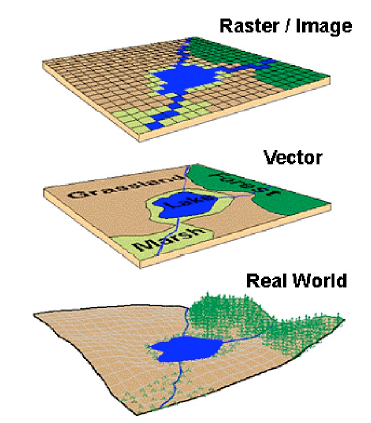
\includegraphics[width=6cm]{Images/Fig_Types_Geodata.png}
    \caption{Vector and raster geographical representation \citep{saabConceptualizingSpaceMapping2003}}
    \label{fig:Fig_data_types}
\end{figure}


% Include image of types of data: Look in \cite{longleyGeographicInformationScience2015} or use image from Andys book

The main use of geographic information is to represent the relative locations of features through a schematic and visual geographic model. With a certain level of abstraction, detail and scale, geographic modelling (mapping) produces knowledge related to the location and the features of the subject of study \citep{longleyGeographicInformationScience2015}. Hence, a geographic information system (GIS) systematically collects geo-referenced attribute data. Gifted with powerful processing capabilities, 'GI systems are computer-based tools for collecting, storing, processing, analyzing, and visualizing geographic information' \citep{longleyGeographicInformationScience2015}.

% Geographic model

% enables one to record and represent the location  

% Abstraction and scientific method reference

% Map as a model to represent reality

% Reference to urban modelling for transport

As computing does in most cases, computer-based GIS offers the capacity to process data in a fraction of the time that it would take if it is performed manually. Similarly, the generation and capture capacity of location-related attributes has widespread \citep{longleyGeographicInformationScience2015}, as digital means have expanded to support all kinds of services and activities. The conjunctions of these two circumstances align with the future scenario portrayed by \cite{wilsonFutureUrbanModelling2018} with urban modelling covering new unattended spatial modelling and analysis needs.

The use cases vary enormously when leveraging GIS technology to contribute to a specific topic or situation. As an example of the versatility of GIS to address location-related topics, \citep{longleyGeographicInformationScience2015} listed possible scenarios, which include:

\begin{itemize}
\item Impact assessment of possible transport infrastructure.
\item Shipping route planning optimization.
\item Health services coverage.
\item Location intelligence for retailers shore expansion.
\item National parks and natural resources management.
\item Agriculture resources consumption.
\item National defence resources allocation.
\item Tourism navigation and reviewing tools.
\end{itemize}

The geo-processing involved in GIS modelling relies on various geometrical and mathematical operations. Depending on the modelling process's type, nature and purpose, different computational procedures are performed to transform the inputs into the intended outcomes that hopefully contribute to the area of study. These methods are usually supported by processing algorithms composed of sequential simpler operations like time, distance, length and area computing. 

% As the GIS derive its operation in  geoprocessing workflows, next some examples of the intermediate results are listed:


% \begin{itemize}
% \item Geometric relations related operations.
% \item Aggregation or dis-aggregation across spatial units.
% \item Spatial and non-spatial data interrelation.
% \item Spatial subsetting.
% \item Proximity analysis.
% \item Time travel matrix computation.
% \end{itemize}

% \begin{itemize}
% \item Point pattern analysis.
% \item Spatial correlation analysis.
% \end{itemize}


In that sense, GIS can address a wide range of location-sensitive topics as they enable and support spatial modelling processes to test future scenarios according to the applicable use case.


\section{Accessibility modelling}

The concept of urban accessibility can be defined as the 'with which people can reach places and opportunities – or, conversely, a characteristic of places and opportunities in terms of how easily they can be reached by the population', \cite{geursAccessibilityEvaluationLanduse2004b} and \cite{neutensEquityUrbanService2010}. Alternatively, \cite{paezMeasuringAccessibilityPositive2012} further expands the definition by framing accessibility into two main components: 'the cost of travel...and the quality/quantity of opportunities'. The cost of travel can be understood as either the monetary cost or the duration or time of the trip to reach the destination, depending on the modelling setup and purpose.

It is important to realize that the universal meaning of accessibility can represent different concepts. \cite{pereiraIntroductionUrbanAccessibility2023a} presented how accessibility can be understood differently depending on the scale and the context where it is applied. On one hand, macro or urban accessibility refers to the effortless ability of people to reach locations of interest. On the other hand, micro-accessibility is related to how spaces are suitable for people with different levels of mobility or reasoning challenges. 


% Mobility vs accessibility

Likewise, accessibility and mobility are terms constantly used in the transport assessment context representing different concepts. Their main distinctive feature can be summarized 
as 'Accessibility,..., refers to the potential ability to reach activities and opportunities. While a mobility analysis would focus, for example, on the time people spend commuting...' \cite{pereiraIntroductionUrbanAccessibility2023a}. Regarding the benefits of introducing accessibility measures in transport planning, \cite{ferreiraAccessibilityGoldMobility2012} argued that planning practitioners should include accessibility measures as they better capture the real benefits in transport-related assessment.


From a global perspective, the aggregate results that urban accessibility provides can also be used to measure sustainability-related contributions. As the measure encapsulates the interaction between transport and opportunities, it explicitly relates to sustainability development goal \# 11 'Make cities and human settlements inclusive, safe, resilient and sustainable' \citep{unitednations17GOALSSustainable2015}. Under this sustainability development goal (SDG), both topics 'Sustainable transport' and 'Sustainable cities and human settlements' are aligned with accessibility measurements, considering that they quantitatively capture the principles that these topics promote.

There are references in the urban development field regarding the interpretation and use of accessibility-based measures.  

\cite{pereiraIntroductionUrbanAccessibility2023a} highlighted how it holistically captures the transportation offer's overall result, the distribution of strategically important activities and the location of individuals within the study area. Additionally, \cite{pereiraIntroductionUrbanAccessibility2023a} stated how accessibility is also related to social inclusion as it accounts for not only the current functioning transport system but also how this system allows individuals to access the location of their interest.

\cite{papaAccessibilityInstrumentsPlanning2016} and \cite{boisjolyHowGetThere2017} stated how accessibility measures are used in transport assessment contexts. \cite{boisjolyHowGetThere2017} presented how accessibility measures favour a more systematic assessment of transportation needs being covered, although their use has not been widespread among transport planning practitioners as the authors expected. \cite{boisjolyHowGetThere2017} considered transport plans from cities in Europe, North America, Australia and Asia.
In contrast, \cite{papaAccessibilityInstrumentsPlanning2016} showcased several European examples where accessibility measures were included in the assessment in routine planning practices.

% Brief explanation of accessibility measures

Within accessibility, multiple measures are available to model how easily people can reach their destinations of interest. \cite{paezMeasuringAccessibilityPositive2012} and \cite{dijstOpportunitiesTransportMode2002} presented a general review of the main groups of accessibility measures, which are summarized and listed next:

\begin{itemize}
  \item Place-based measures: The place-based measures aim to quantity the ability to reach opportunities from a specific location in space due to the spatial distribution of opportunities and the transport network available. These measures can be grouped as follows:
    \begin{itemize}
        \item Cumulative opportunity measures: The cumulative measure considers the total of opportunities that can be reached from a given location that complies with a time or travel cost threshold.
            \begin{itemize}
                \item Active cumulative accessibility measure: It consists of the number of opportunities a person in a given location can easily access within a threshold. 
                \item Passive cumulative accessibility measure: It reflects the number of people that can reach a certain destination or opportunity without exceeding the travel cost threshold.
            \end{itemize}
        \item Minimum travel cost: It maps the nearest locations of interest (opportunity) by considering the one destination with the lowest travel cost, either time or monetary.
        \item Gravity measures: Based on Newton's gravitational model, it accounts for variation in travel cost as the distance between the origin and destination location increases.
        \item Floating catchment area competition: The catchment area measure aims to account for the interaction between the offer of opportunities and the demand of individuals according to their spatial distribution and accessibility levels.
        
    \end{itemize}
  \item Person-based measures: In conjunction with the transport network and spatial opportunity distribution, this measure also considers the personal features of individuals in a given location in space.
\end{itemize}

\section{Colombia and the Bogot\'{a} study case}

In urban development, there is an extended list of references related to accessibility applied to transport assessment contexts. Particular interest in research activities has been expended on areas that have experienced migration and/or relatively more rapid urbanisation processes \citep{kojimaIntroductionPopulationMigration1996}. Latin America and Colombia are not excluded from this trend as the rapid urbanization reinforces the already present inequalities in cities \citep{wrightwendelAccessibilityUsabilityGreen2012,tellezUrbanDevelopmentBogota2018}.


Colombia's capital, Bogot\'{a} has been an area of study of multiple transport and accessibility-related research exercises. That should not come as a surprise considering the population growth that Bogot\'{a} and her surrounding municipalities have experienced over the last couple of decades. By 2017, Bogot\'{a} had almost doubled its population during the last 30 years and similarly did the nearby municipalities by increasing their population by almost 3 times during the same period \citep{guzmanCityProfileBogota2017}.

A milestone in Bogotá's transportation history was the operation start of its current BRT 'Transmilenio' system by the beginning of the 21st century \citep{rodriguezValueAccessibilityBogota2004}. Derived from the deployment and the integration of collective bus services in Bogotá, the resulting accessibility effect of the BRT system has been a popular element of study among transport and development-related researchers. The next paragraph intends to explore the previous research exercises that have expanded on the present research topic of interest. However, there are clearly other valuable contributions that could not be included due to practical limitations.

% It is clear that the BRT system provided the city with a functioning solution to integrate most of the collective bus services.

Although it was not a proper accessibility assessment as defined in previous sections, \cite{rodriguezValueAccessibilityBogota2004} initially examined the relationship between proximity and land value and found that apparently there was a positive relation between the land price and the proximity to the BRT system stations. However, the influence might be underscored by the short time frame (2 years) between the measure and the operation kick-off of the BRT system.

With a more straightforward social-inequality and accessibility approach, \cite{bocarejos.TransportAccessibilitySocial2012} performed an urban accessibility assessment on the city's BRT system. Considering that their main research goal was to generate an 'analysis tool that helps quantify and differentiate access inequalities' \cite{bocarejos.TransportAccessibilitySocial2012} highlighted the value of introducing the accessibility concept as part of the analysis. Additionally, the authors also considered economic individual constraints that the users might have to 'consider not only an indicator that relates the transport system to land use, but the real possibility of transport use and ease of access to the city opportunities depending on individual purchasing power' \cite{bocarejos.TransportAccessibilitySocial2012}.

In a further exercise, \cite{bocarejoAccessibilityAnalysisIntegrated2014} expanded on the accessibility assessment by including additional variables related to the use and related benefit of the BRT system in Bogotá. As the BRT system progressively expanded and integrated more auxiliary routes intended to feed the main corridors of the system, their research purpose was to assess the impact of the integration in accessibility terms. As the integration of the auxiliary routes with the main BRT network was a novel situation at the time, \cite{bocarejoAccessibilityAnalysisIntegrated2014} included further variables in the assessment like the purchasing power of the users and cost/benefit ratio considering multiple possible fare schemes. The results confirmed the relevance of the use of accessibility measures as they found that the integration generated time reductions in the periphery areas of the city; however, affordability constraints can materialize in low-income users \citep{bocarejoAccessibilityAnalysisIntegrated2014}.

Similarly, with a social and equality accessibility approach, \cite{guzmanAssessingEquityTransport2017} performed an accessibility assessment at a more regional scale. Not only considering Bogotá capital district municipality, \cite{guzmanAssessingEquityTransport2017} included the surrounding municipalities for a more regional-cohesive result. Additionally, privately owned cars, ordinary buses and BRT transportation modes were disaggregated to assess accessibility individually. Regarding the opportunities, that means the destination of interest,\cite{guzmanAssessingEquityTransport2017} particularly focused on jobs and education-related points of interest.

Subsequently, \cite{guzmanAccessibilityAffordabilityEquity2018} carried out a transport accessibility assessment that considered multiple fare subsidy scenarios. By formulating a possible fare subsidy scheme, \cite{guzmanAccessibilityAffordabilityEquity2018} spatially modelled the effect in affordability and accessibility derived from using the public transportation network.

The main common purpose of previous research conducted in Bogotá was to assess the accessibility impact of the transportation system's future expansion, integration or fare scheme introduction. The accessibility measures were mostly assessed from a social and access-inequality perspective as results were disaggregated by population groups of interest.



\chapter{Data} \label{Chap3}

% \begin{itemize}
%   \item Brief context of Bogot\'{a} as Colombia\textquotesingle s capital
%   \item Current Bogot\'{a}\textquotesingle s spatial structure
%   \item Social and spatial population distribution
% \end{itemize}

\section{Summary}

Considering the main components that influence the accessibility measures \citep{pereiraIntroductionUrbanAccessibility2023a}, Table \ref{tab:Data_summary} groups the primary input used to develop the present research project, respectively, while indicating the source in each case.

\begin{table}[H]
\centering
\renewcommand{\arraystretch}{1.6} % Adjust the row height
\resizebox{\textwidth}{!}{%
\begin{tabular}{llll}
\hline
\multicolumn{1}{c}{\textbf{Component}} &
  \multicolumn{1}{c}{\textbf{Input}} &
  \multicolumn{1}{c}{\textbf{Description}} &
  \multicolumn{1}{c}{\textbf{Source}} \\ \hline
\multirow{3}{*}{\begin{tabular}[c]{@{}l@{}}Transport \\ infrastructure\end{tabular}} &
  BRT system &
  Static transit information of current system &
  \cite{transmilenios.a.GTFSEstaticos202306212023} \\
             & Road and walking network & Street network                         & \cite{openstreetmapcontributorsPlanetDumpRetrieved2023} \\
             & Metro system             & Track and station data of future metro & \cite{alcaldiadebogotad.c.TrazadoPrimeraLinea2022,alcaldiadebogotad.c.EstacionesPrimeraLinea2022} \\ \hline
Land use     & Predominant land use     & Predominant use terrain level data     & \cite{alcaldiadebogotad.c.DestinoEconomicoPredominante2022} \\ \hline
Demographics & Multipurpose survey      & Anonymized survey data                 & \cite{secretariadistritaldeplaneacionMicrodatosEncuestaMultiproposito2023,secretariadistritaldeplaneacionCapaGeograficaEncuesta2023} \\ \hline
\end{tabular}}
\caption{Input data summary.}
\label{tab:Data_summary}
\end{table}

The local government of Bogotá (Alcaldia de Bogotá D.C.) generated, directly or indirectly, most of the input information used to model accessibility. The transport infrastructure component groups the data that describes the current and future transportation network of Bogotá. In the case of the transit data used to model the operation of the current BRT network, it was generated and published by Transmilenio S.A., which is a publicly owned company in charge of managing and coordinating the BRT system operation \citep{transmilenios.a.HistoriaTransmilenioHistory2013}. Regarding the Multipurpose Survey information in the demographic component, it was jointly gathered by the Planning Department of Bogotá City Council (Sectretaría Distrital de Planeación) and the National Administrative Statistics Department (Departamento Administrativo Nacional de Estadística - DANE).


The following sections contain a general description of each input data used to model accessibility.





\section{Transport infrastructure}

\subsection{BRT network}

The transit information from the current BRT network systematically both the infrastructure and the transport operation. As the entity responsible for managing the operation of the BRT system, Transmilenio S.A. has published\footnote{Transit information dated 21/06/2023} their transit using a GTFS\footnote{GTFS: General transport feed specification} format. The GTFS format is an open-source standardized format that describes transport operations' main features. Numerous transport agencies currently use this format as it integrates spatial data, fleet, fare and timetables \citep{pereiraIntroductionUrbanAccessibility2023a, mobiltydataGeneralTransitFeed2023}.

GTFS data comprises tables containing spatial and non-spatial features of the transportation system. Through key fields to trace relationships between the multiple tables, GTFS characterises multimode systems, their routes, fares, frequencies, and timetables, among other features. For example, Figure \ref{fig:GTFS_structure} illustrates the general structure of GTFS data and how the tables relate. Similarly, Table \ref{tab:GTFS_description}, describes the main features of every table in the GTFS data structure.

Important to note the relation between route and trip information in the GTFS data structure, presented in \ref{tab:GTFS_description}. The route table indicates the routes that compose the transport system. In a similar matter but at a lower transport system hierarchy level, trips should be understood as transport service units comprising each route \citep{pereiraIntroductionUrbanAccessibility2023a}. In other words, the trip service units are how the transport operation of each route materializes.

\begin{figure}[H]
    \centering
    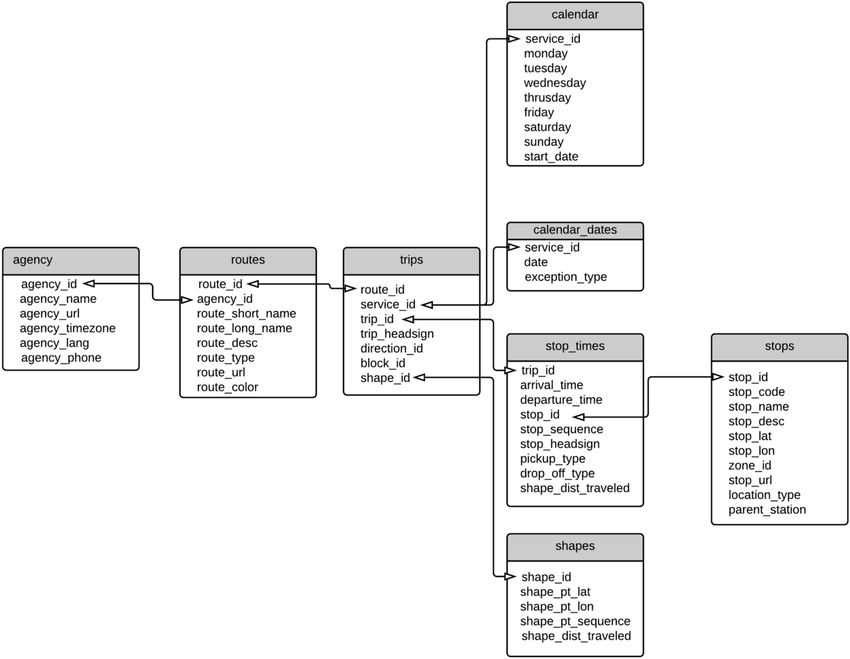
\includegraphics[width=10cm]{Images/GTFS-data-format.png}
    \caption{GTFS data structure (\cite{pereiraExploringTimeGeography2023} cited by \cite{pereiraIntroductionUrbanAccessibility2023a})}
    \label{fig:GTFS_structure}
\end{figure}

\begin{table}[htp]
\centering
\renewcommand{\arraystretch}{1.5} % Adjust the row height
\resizebox{\textwidth}{!}{%
\begin{tabular}{lll}
\hline
\multicolumn{1}{c}{\textbf{Table name}} & \multicolumn{1}{c}{\textbf{Topic}} & \multicolumn{1}{c}{\textbf{Description}}                  \\ \hline
agency                                  & Transport providers                & General transport providers data including transport mode \\ \hline
routes          & Routes information        & Transit routes of the system                     \\ \hline
trips           & Trips information         & Unit of transit service for routes of the system \\ \hline
shapes          & Route geometry            & Route path spatial information                   \\ \hline
stops           & Stations                  & Spatial location of stations                     \\ \hline
stops\_times                            & Trip schedule                      & Arrival and departure time of trips in each station       \\ \hline
frequencies     & Frequencies of trips      & Service frequencies of each trip                 \\ \hline
calendar        & General calendar schedule & Weekday general service scheduling               \\ \hline
calendar\_dates                         & Specific calendar schedule         & Special inclusions or exceptions in service scheduling    \\ \hline
fare\_attibutes & Fare description          & General fare conditions                          \\ \hline
fare\_rules     & Fare class description    & Class and fare parameters                        \\ \hline
\end{tabular}}
\caption{GTFS tables general description \citep{mobiltydataGeneralTransitFeed2023}}
\label{tab:GTFS_description}
\end{table}

% map of BRT geometries
Figure \ref{fig:BRT_route_type} shows that Bogotá's BRT network comprises a multilevel route network. Apart from the main corridor BRT network, the system has been expanded into additional complementary routes that are described next:

\begin{itemize}
  \item Main: The route under the main category consists of the exclusive lane routes in the main corridors of the system.
  \item Feeder: The feeder routes are bus routes that use non-exclusive lanes in the road network. Their main role in the system is to connect nearby areas with the main corridors.
  \item Urban: The urban routes offers bus transit services across the city using non-exclusive road lanes.
  \item Complementary and Special: These routes also use non-exclusive lanes from the road network and their grouping category is more related to system operation management.
\end{itemize}

\begin{figure}[H]
    \centering
    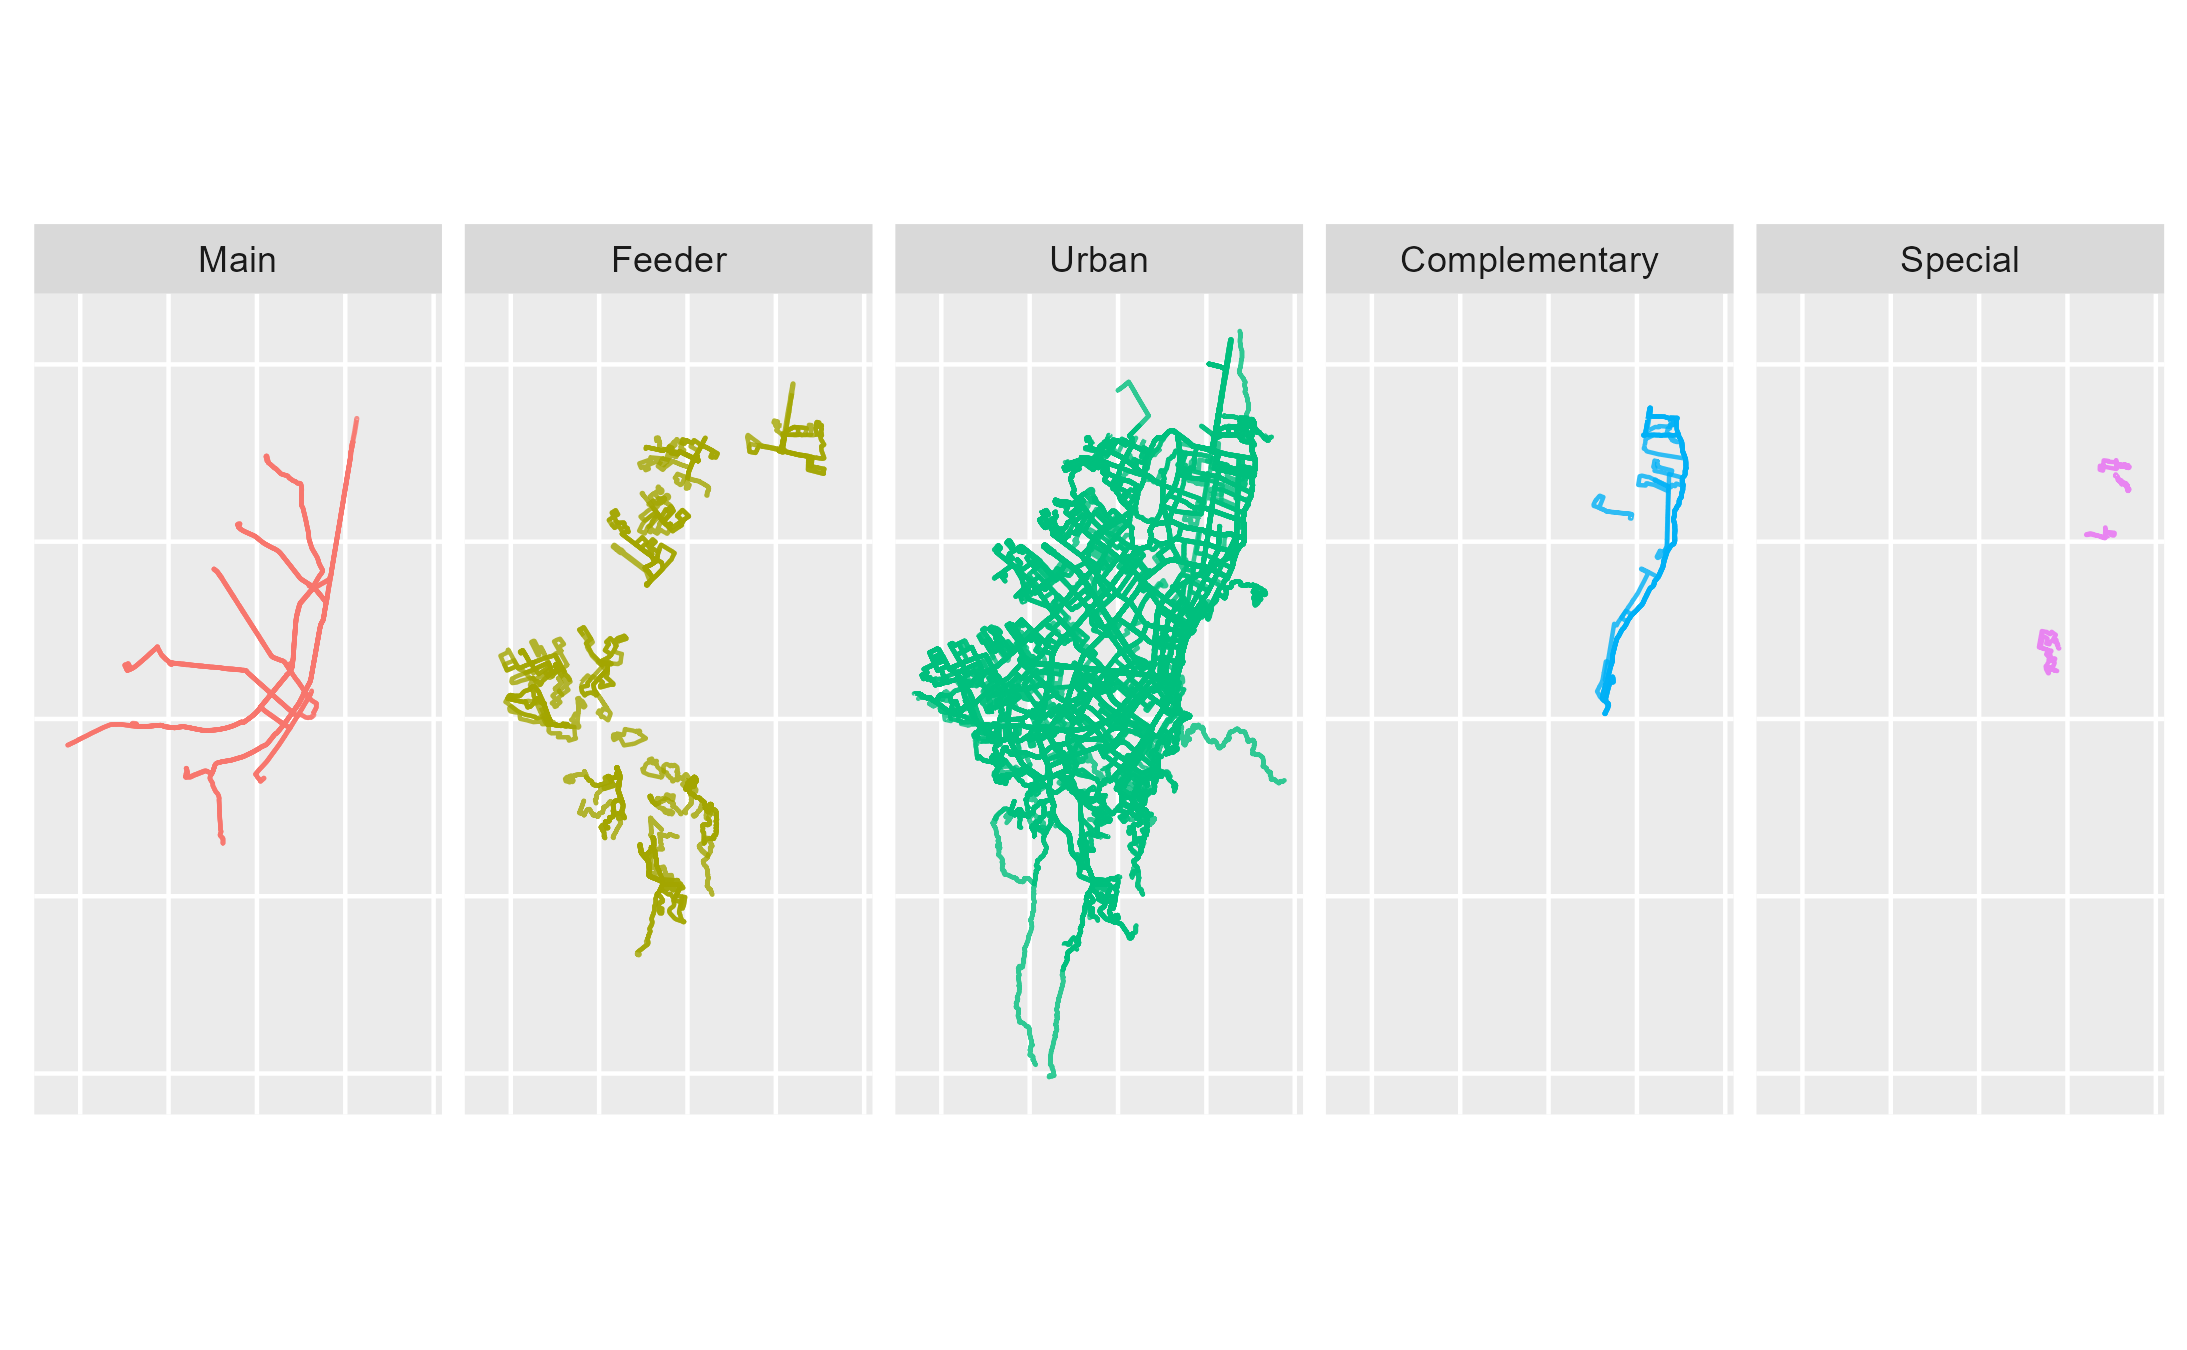
\includegraphics[width=15cm]{Data/Results/Images/BRT_Network_Route.png}
    \caption{BRT network by route type \citep{transmilenios.a.GTFSEstaticos202306212023}}
    \label{fig:BRT_route_type}
\end{figure}

\subsection{Road and walking network}

As commuting practices rely upon more than one mode of transportation, the modelling process requires considering the mode available to reach the desired destinations from the trip's origin. To access a motorized transport mode or make complete mono mode trips, walking constitutes an essential element when modelling commuting trips, therefore, in the accessibility modelling process.

The road and walking network of Bogotá was taken\footnote{Extracted data dated 01/07/2023.} from Open Street Map (OSM) available through \cite{hotexporttoolHOTExportTool2023}. All the transport-related available features were extracted to replicate the possible physical infrastructure for walking. The data format in which the data was downloaded is Protocol Binary Format (PBF), the OSM native vector data format.

\begin{figure}[H]
    \centering
    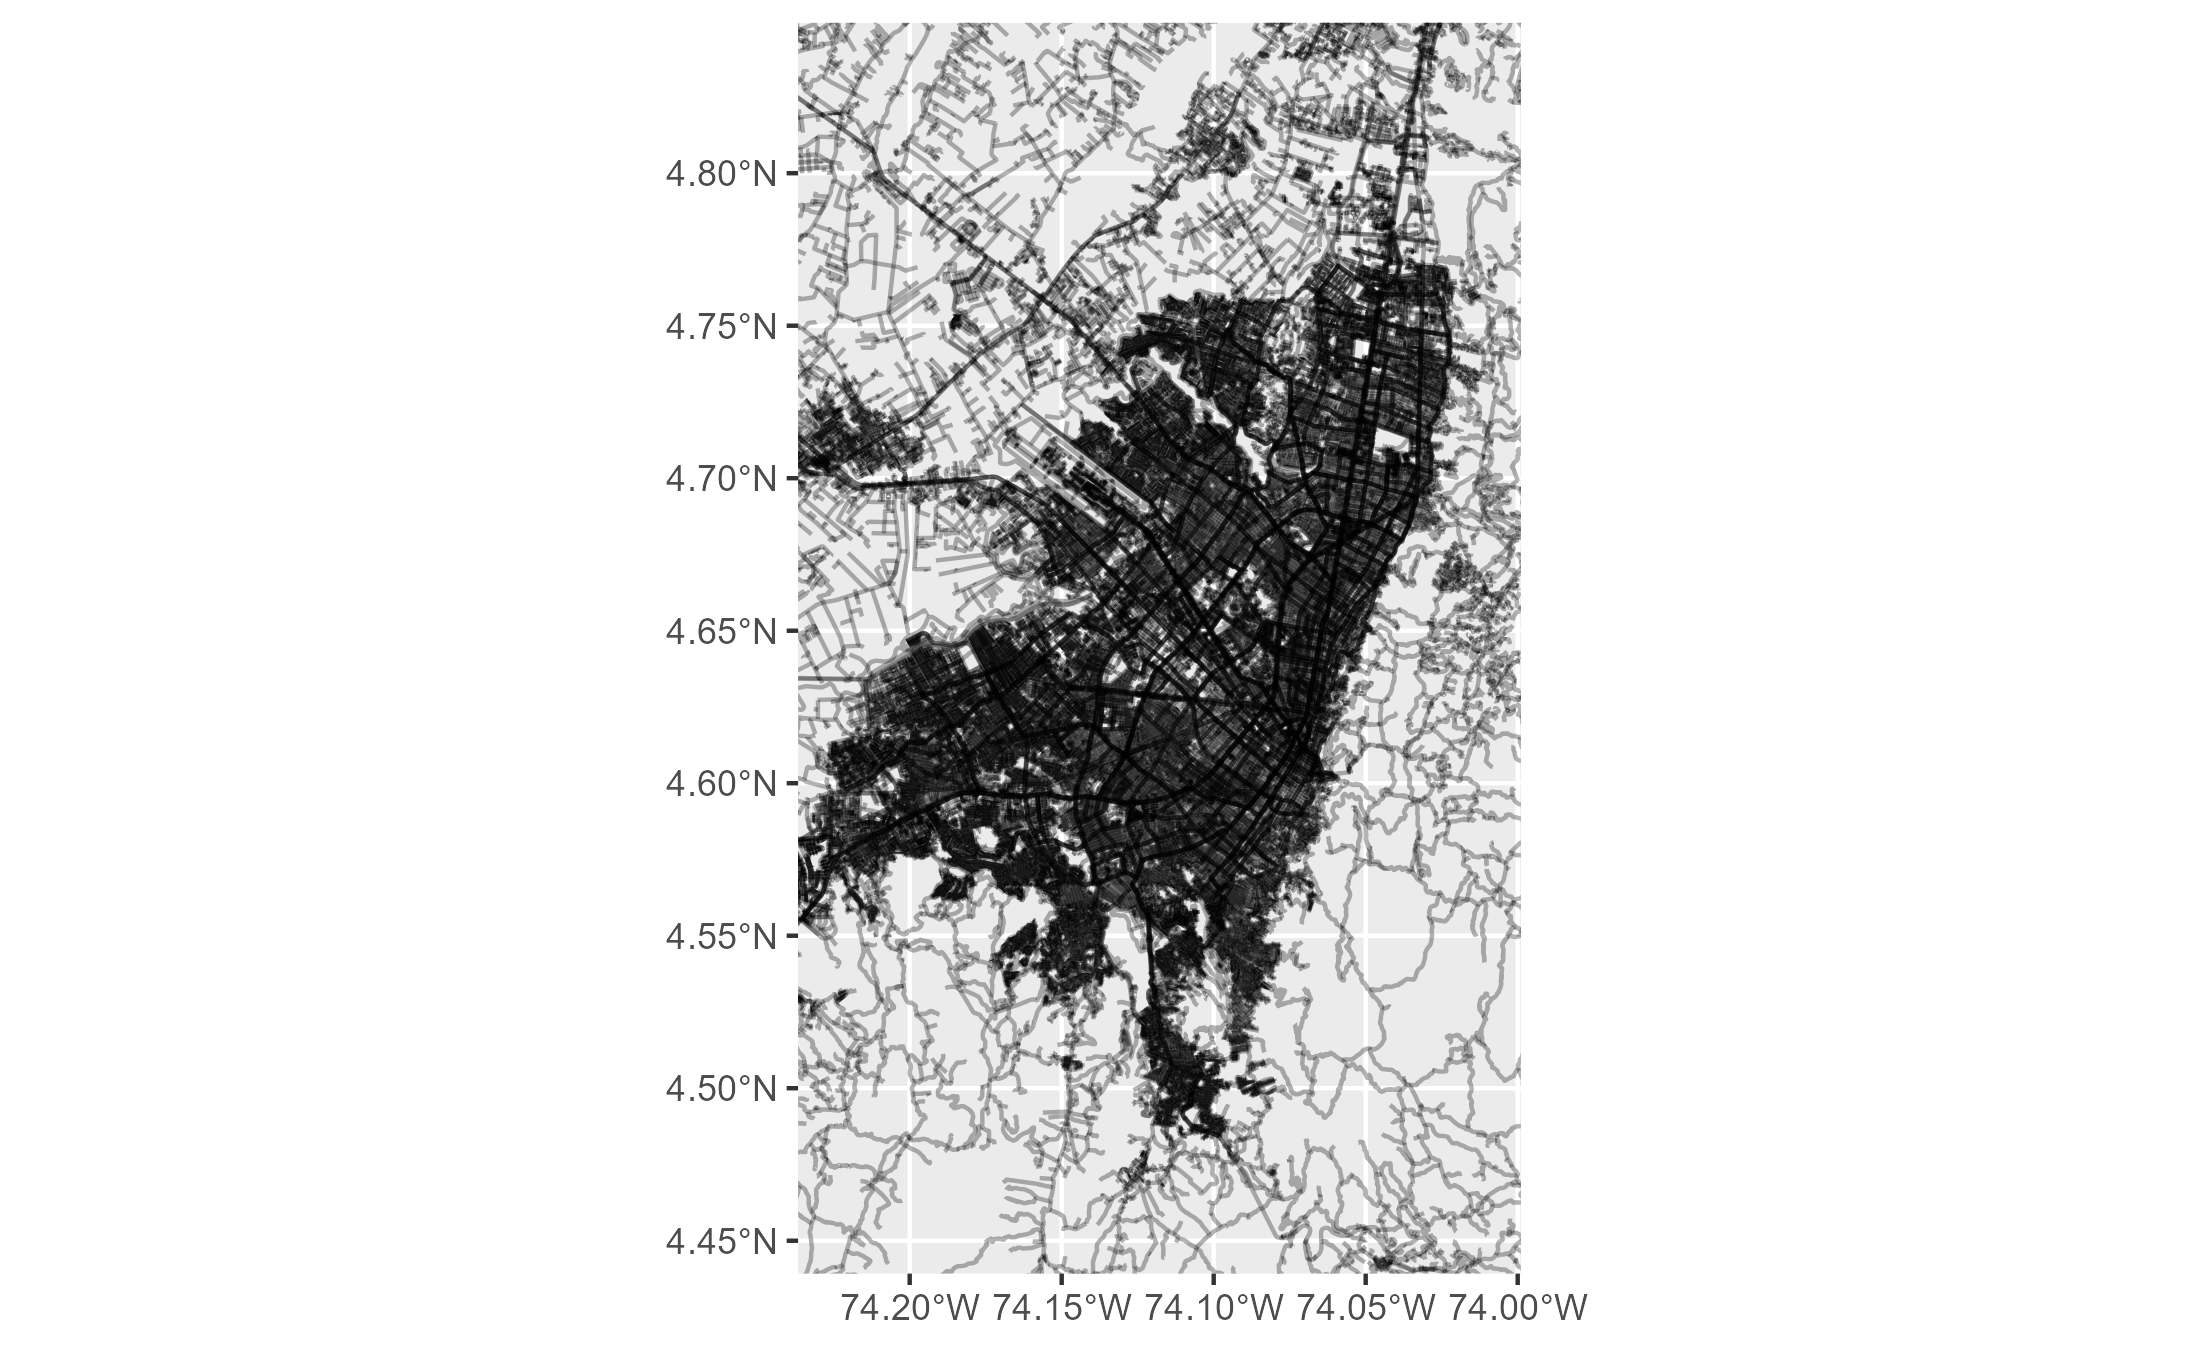
\includegraphics[width=15cm]{Data/Results/Images/OSM_Network.png}
    \caption{Street network infrastructure \citep{openstreetmapcontributorsPlanetDumpRetrieved2023}}
    \label{fig:OSM_Network}
\end{figure}

Figure \ref{fig:OSM_Network} shows an overview of the transport-related infrastructure of Bogotá extracted from OSM. 

% no subsetting
% Closest to reality
% Refence to vector data

\subsection{Metro network}

The metro transport infrastructure data was taken from the publicly available designs of the first line of the future metro. Bogotá city council has published the spatial data related to the main features of the future metro system. The spatial information includes the location of the stations and the geometry track path.

Figure \ref{fig:Metro_Network} presents the track locations, stations, and Bogotá municipal boundary. The 23.9-kilometre length track line follows a north-south direction in the east zone of the city to later connect the east-south and west-south of Bogotá.

\begin{figure}[H]
    \centering
    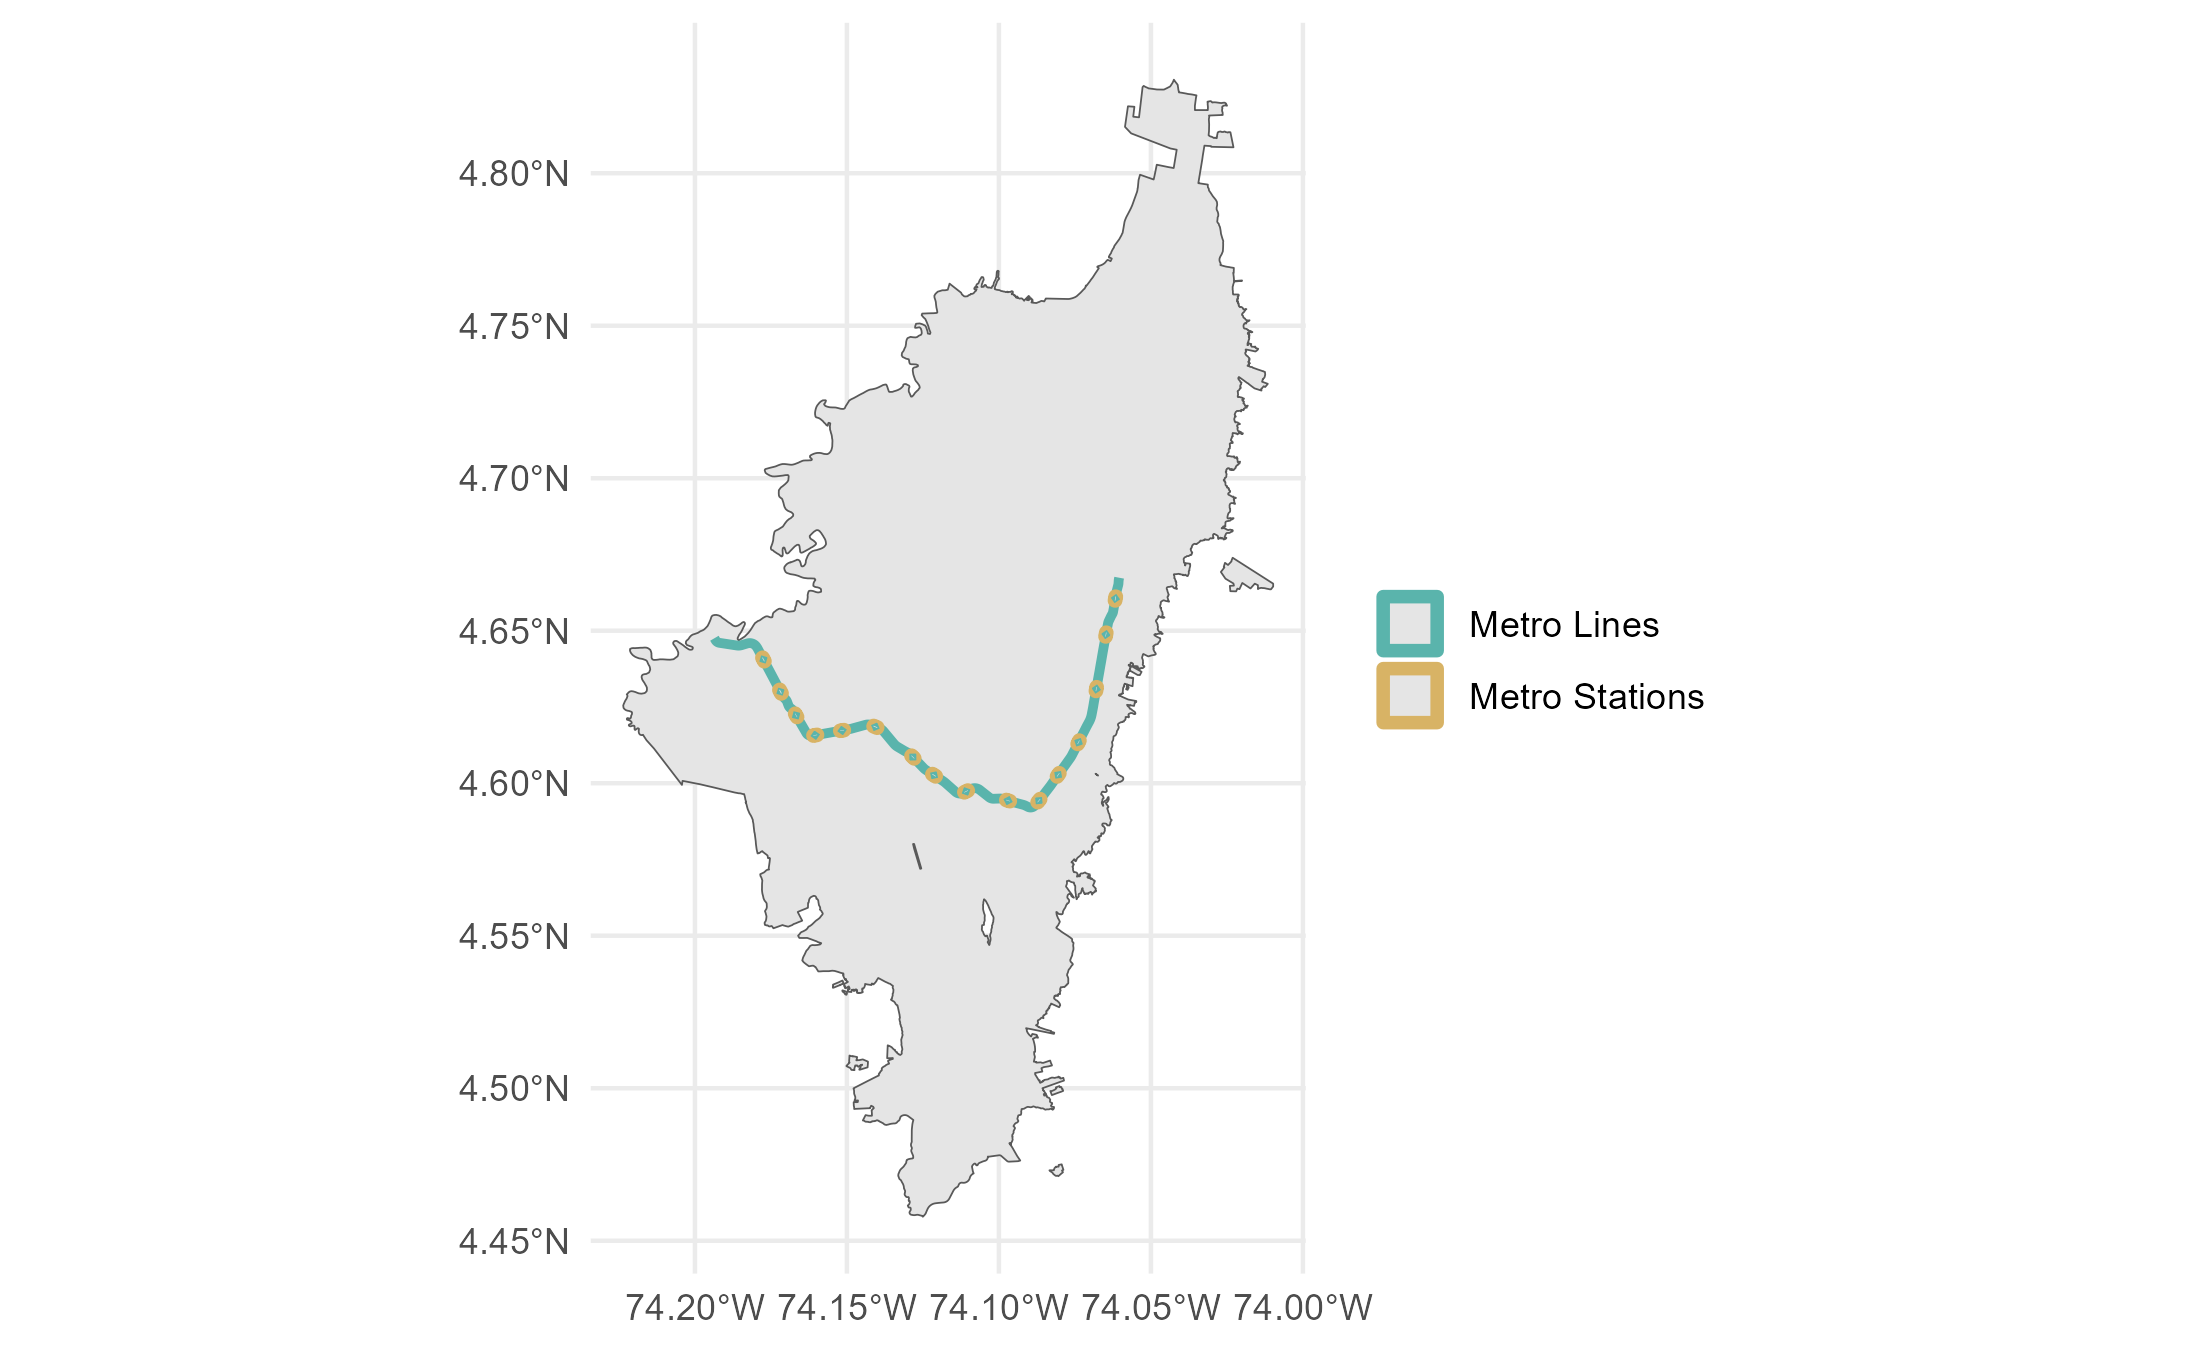
\includegraphics[width=15cm]{Data/Results/Images/Metro_Network.png}
    \caption{Future metro infrastructure \citep{alcaldiadebogotad.c.EstacionesPrimeraLinea2022, alcaldiadebogotad.c.TrazadoPrimeraLinea2022}}
    \label{fig:Metro_Network}
\end{figure}

\section{Land use}

Land use data allows classifying properties according to their predominant economic use. Through terrain spatial data published by \cite{alcaldiadebogotad.c.DestinoEconomicoPredominante2022} it is possible to compute the spatial distribution of properties by their primary land use. Figure \ref{fig:Land_Use_Commercial} shows the spatial distribution of terrains in Bogotá classified as commercial corridor land use, with clusters mainly in the east zone of Bogotá. 

\begin{figure}[H]
    \centering
    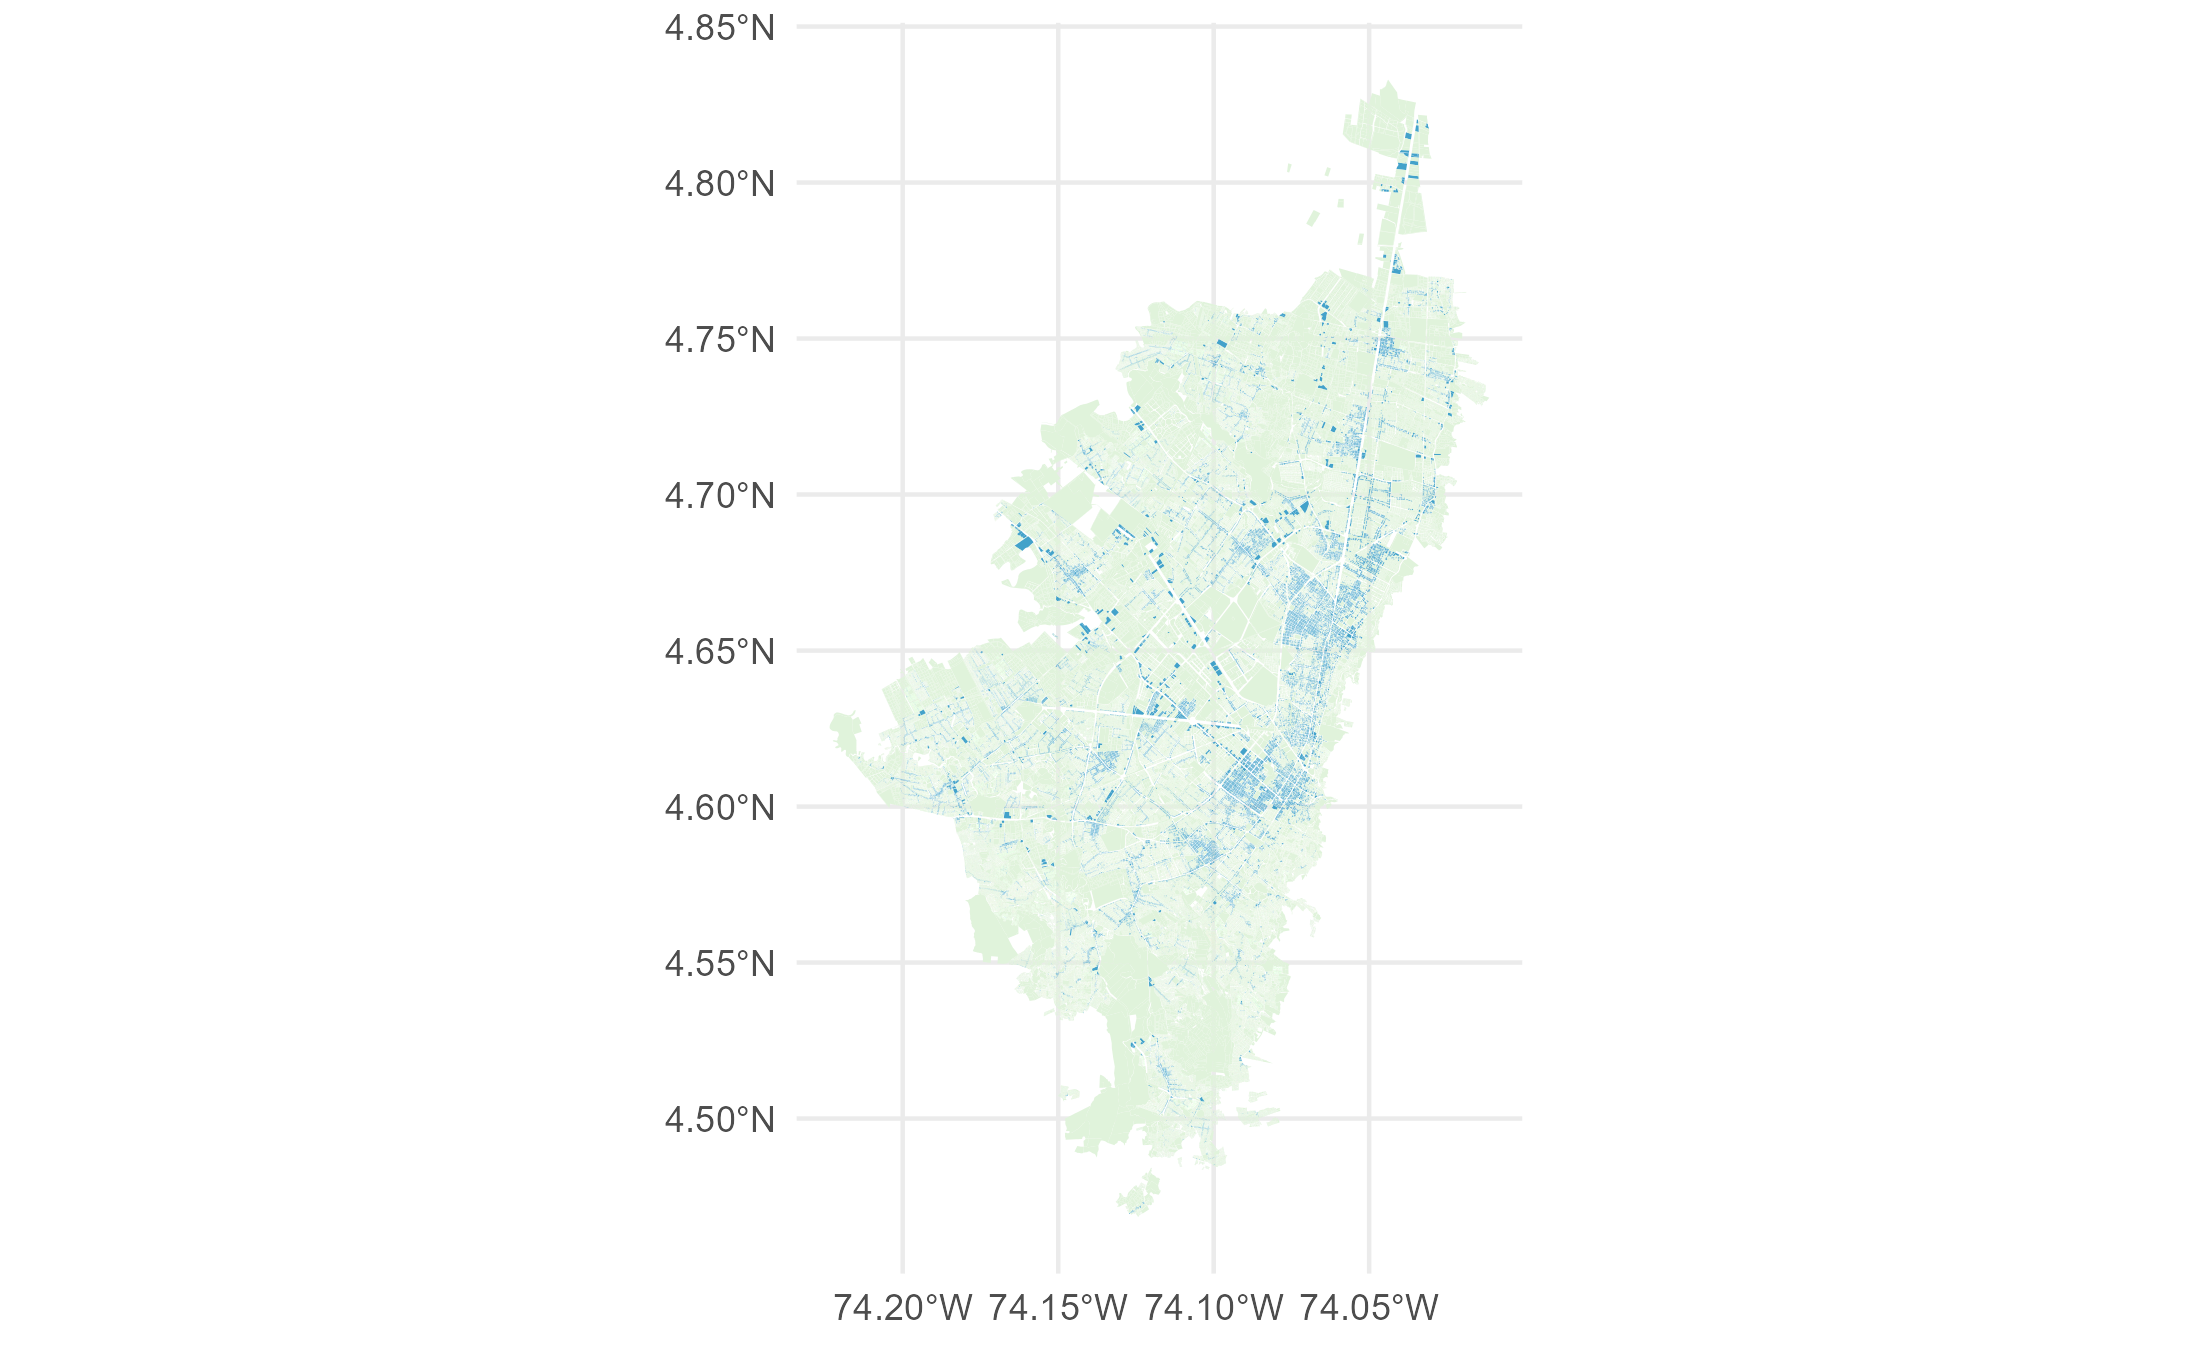
\includegraphics[width=15cm]{Data/Results/Images/Land_Use_Commercial_Corridor_Terrain.png}
    \caption{Terrains with commercial corridor land use \citep{alcaldiadebogotad.c.DestinoEconomicoPredominante2022}}
    \label{fig:Land_Use_Commercial}
\end{figure}

\section{Demographics}

% Reference to the survey
% Reference to the GIS layer

With a multipurpose approach, \cite{secretariadistritaldeplaneacionCapaGeograficaEncuesta2023} gathered information through a survey from Bogotá's households. The multipurpose survey captured multiple variables at a residential, household and personal level of Bogotá's population. Among the topics covered in the survey it included variables related to living conditions, housing, utilities, health, education and demographics.

The survey data has been gone through an anonymization procedure done by \cite{secretariadistritaldeplaneacionMicrodatosEncuestaMultiproposito2023} to keep non-spatial and spatial attributes unexposed. The residential location of the public surveyed is not published. However, the data can be spatially aggregated by the zoning planning unit (ZPU) used by Bogotá City Council as a spatial-administrative subdivision of their main boroughs. As the survey microdata contains the corresponding ZPU where each survey was collected, it is possible to aggregate the results spatially. 

Figure \ref{fig:Demo_Income_ZPU} present the median household income by ZPU in Bogotá. The highest median income values are registered in the northeast part of the city, while the lowest are found in the south and southwest areas.

\begin{figure}[H]
    \centering
    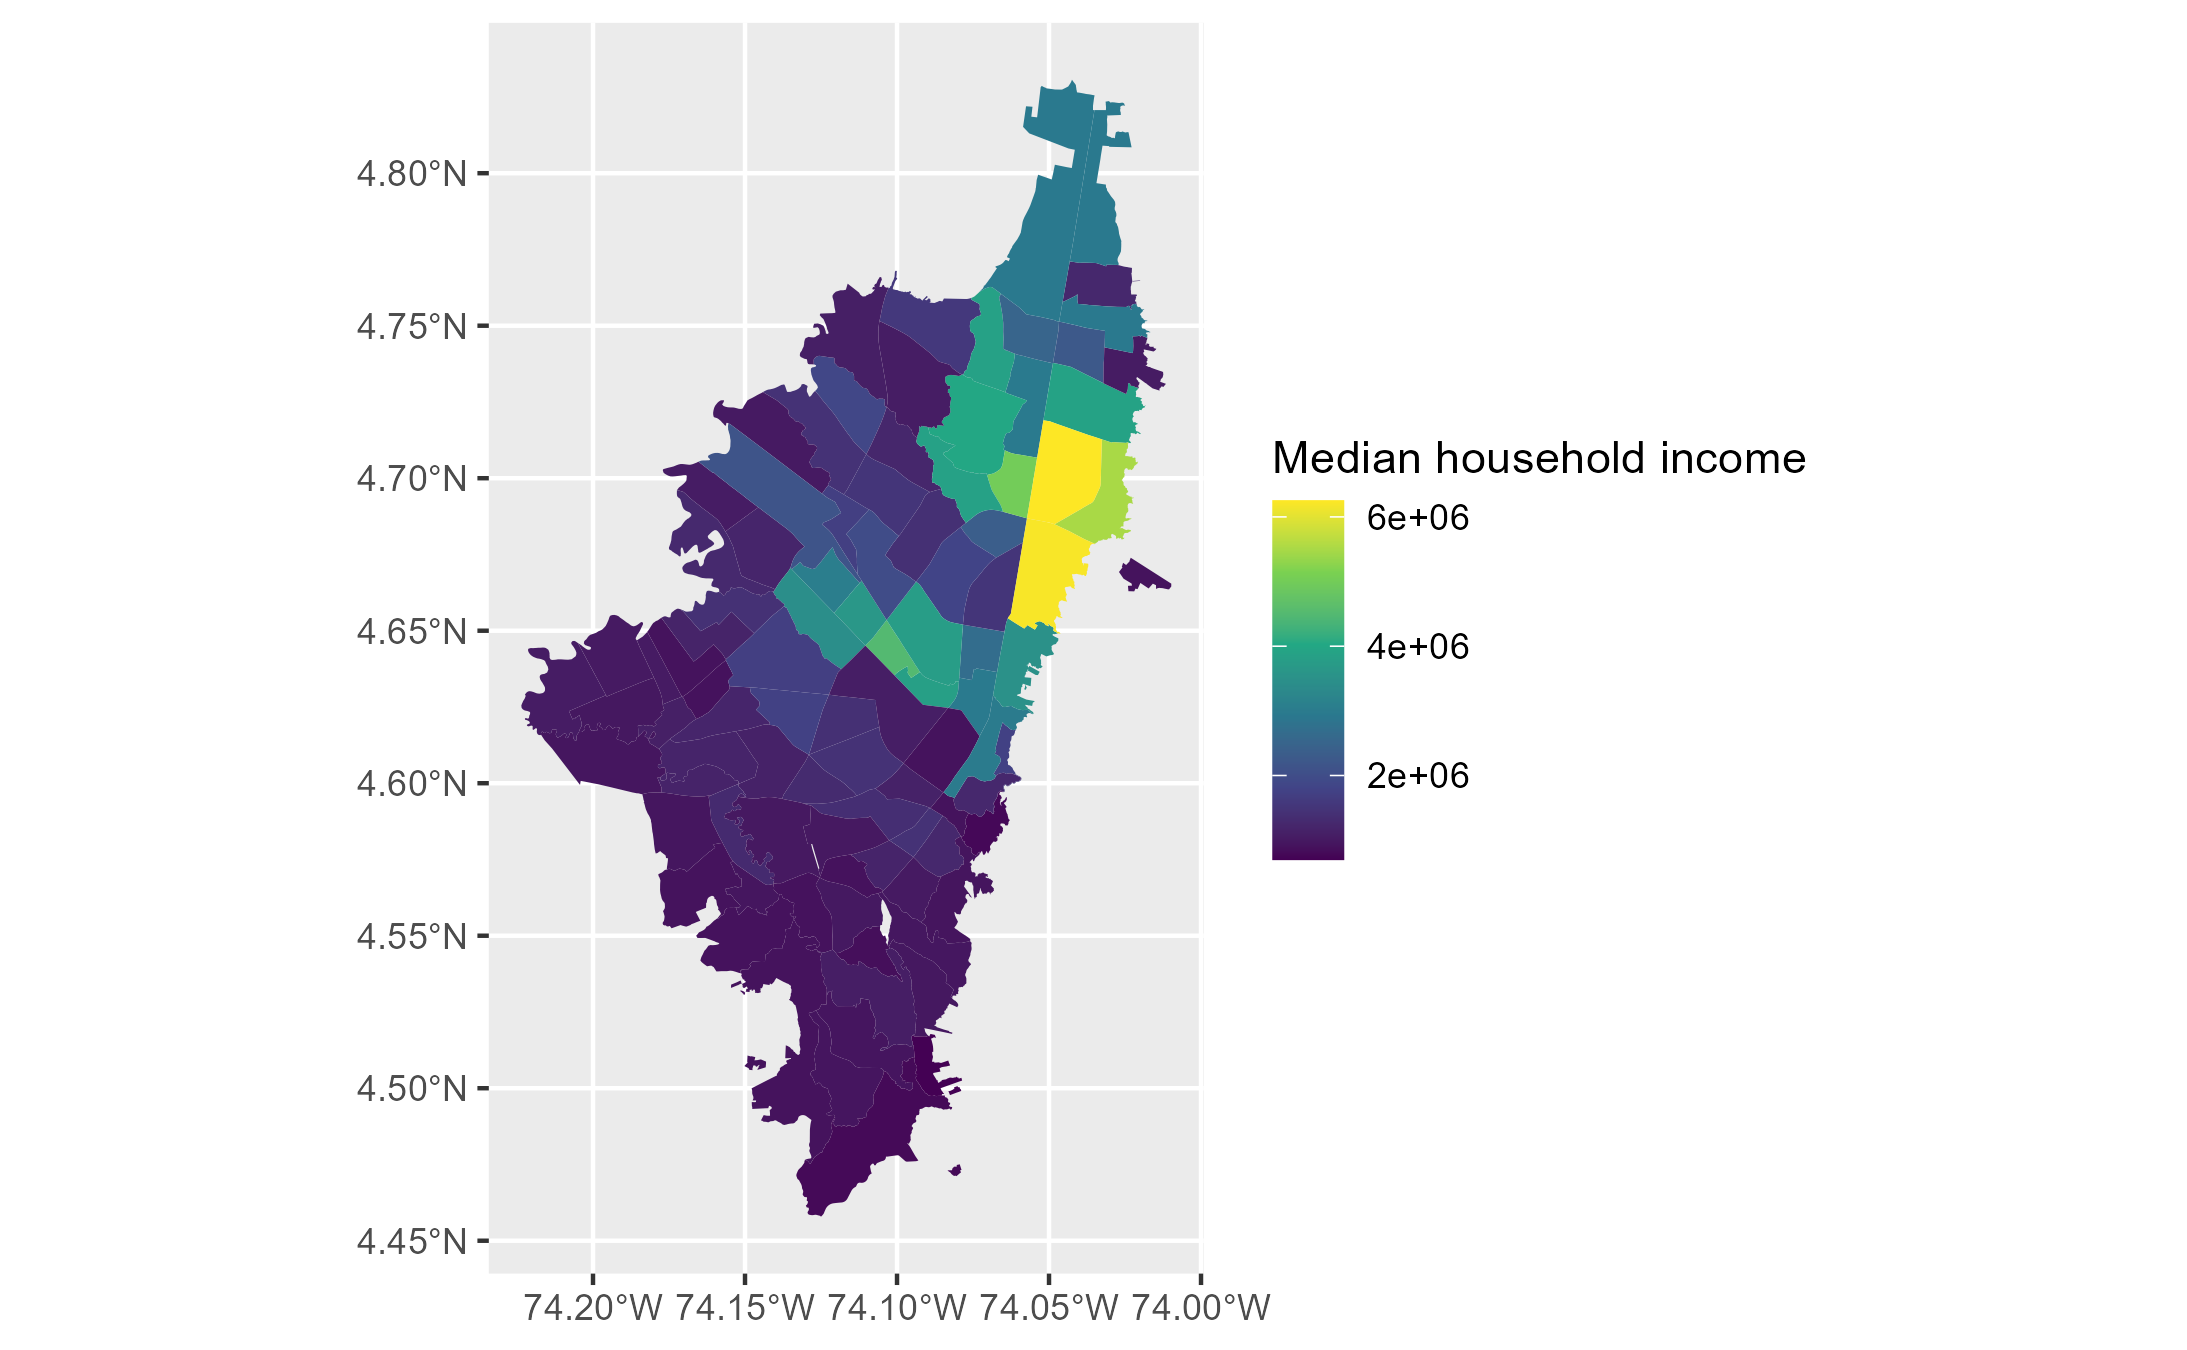
\includegraphics[width=15cm]{Data/Results/Images/Demo_Income_UPZ_Mean_Median.png}
    \caption{Median household income by Zoning Planning Units (ZPU) \citep{secretariadistritaldeplaneacionMicrodatosEncuestaMultiproposito2023, secretariadistritaldeplaneacionCapaGeograficaEncuesta2023} }
    \label{fig:Demo_Income_ZPU}
\end{figure}


\chapter{Methodology} \label{Chap4}


\section{Overview}

The literature explored above presents an overview of how urban modelling enables future scenario assessment that can reorient transport-related planning practices by introducing accessibility measures. Strictly mobility-based transport policymaking practices can fall short of fully assessing the real tangible benefits of transport infrastructure projects. Additionally, inhabitants' spatial distribution and socioeconomic conditions can differ dramatically within the urban context. As a result, the accessibility measurement result denotes a different level of deprivation and urgency outlook depending on the living conditions identified in the location of interest. Therefore, apart from introducing accessibility-based measures when assessing transport infrastructure projects, the results should be disaggregated into population groups of interest who might be experiencing the most precarious living conditions. For this reason, prioritizing relative accessibility improvements across population groups experiencing a higher degree of deprivation or vulnerability should be considered when promoting any transport-related initiative.


Hence, this study measured urban accessibility for the current and future metro scenario in Bogotá, Colombia. Using a before and after comparison analysis, this research calculated the accessibility improvement derived from the future transit operation of Bogotá's metro system, combined with the current functioning BRT network.

\begin{figure}[H]
    \centering
    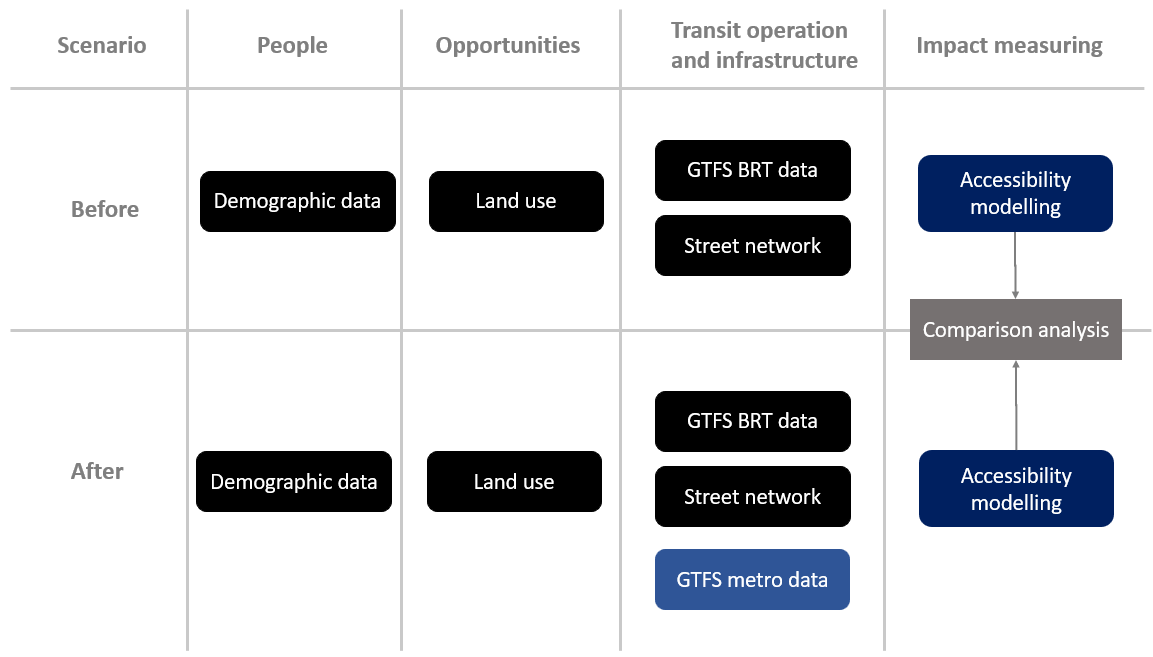
\includegraphics[width=16cm]{Images/Method_Summary.png}
    \caption{Method summary diagram}
    \label{fig:Method_Summary}
\end{figure}

First, this study generated projected transit data for the metro system based on the main features and spatial data already published by Bogotá's local authorities. Second, land use and demographic data are integrated into a spatial framework to track the spatial distribution of economic activity and to assess living conditions in Bogotá's inhabitants spatially. Finally, by integrating transit information from before and after scenarios, the study maps how the accessibility levels will spatially vary by population groups of interest with the construction and operation of the new metro system. The analysis, preprocessing, modelling and visualization process was conducted using R Programming Language. For the accessibility modelling process, the study used the R5R library to produce the results and the accessibility library as a control method.


\section{Ethics}

This research aims to provide urban accessibility-based measurements in a future transport infrastructure scenario to showcase the value of accessibility in transport planning practices and assess the accessibility impact of Bogotá's future metro system.

The information used in this research was publicly available except for a spatial ZPU layer \citep{secretariadistritaldeplaneacionMicrodatosEncuestaMultiproposito2023} from the Multipurpose Survey \citep{secretariadistritaldeplaneacionCapaGeograficaEncuesta2023} which contains demographic information of Bogotá's inhabitants. The geographic ZPU layer was provided directly by Bogotá's Planning Department after formally requesting it for research purposes. The research used the ZPU layer to spatially aggregate demographic data, which will be further used to assess the accessibility result in different population groups.

Neither the survey microdata nor the spatial layer contained traceable data from individuals. In the first place, before publically sharing the results \cite{secretariadistritaldeplaneacionMicrodatosEncuestaMultiproposito2023} performed a spatial and non-spatial anonymization procedure on the survey microdata so the individual information exposure risks were mitigated. In like manner, the GIS layer only contained identification data from the ZPU polygons but not individual-specific data.

This study's aimed contributions fall in the university research domain and pose low ethical risks. In compliance with the ethical risks screening procedure, the
The Departmental Ethics Committee assessed, reviewed and successfully approved\footnote{Approval number CASA23/5032971/1} the data and method considered in this research. 


\section{Area of study}

The geographical area of study is Bogotá City, Colombia's capital. The boundary of Bogotá's capital district will be the physical limit that encloses the spatial study area of this research exercise. Figure \ref{fig:Study_Area_ZPU} presents Bogotá's capital district boundary with the local ZPU\footnote{For consistency purposes, the map shows 96 ZPU as aggregated in the Muliprpuse Survey, although there are official 112 \citep{secretariadistritaldegobiernoCaracterizacionUsuarios20212021}} limits.

\begin{figure}[H]
    \centering
    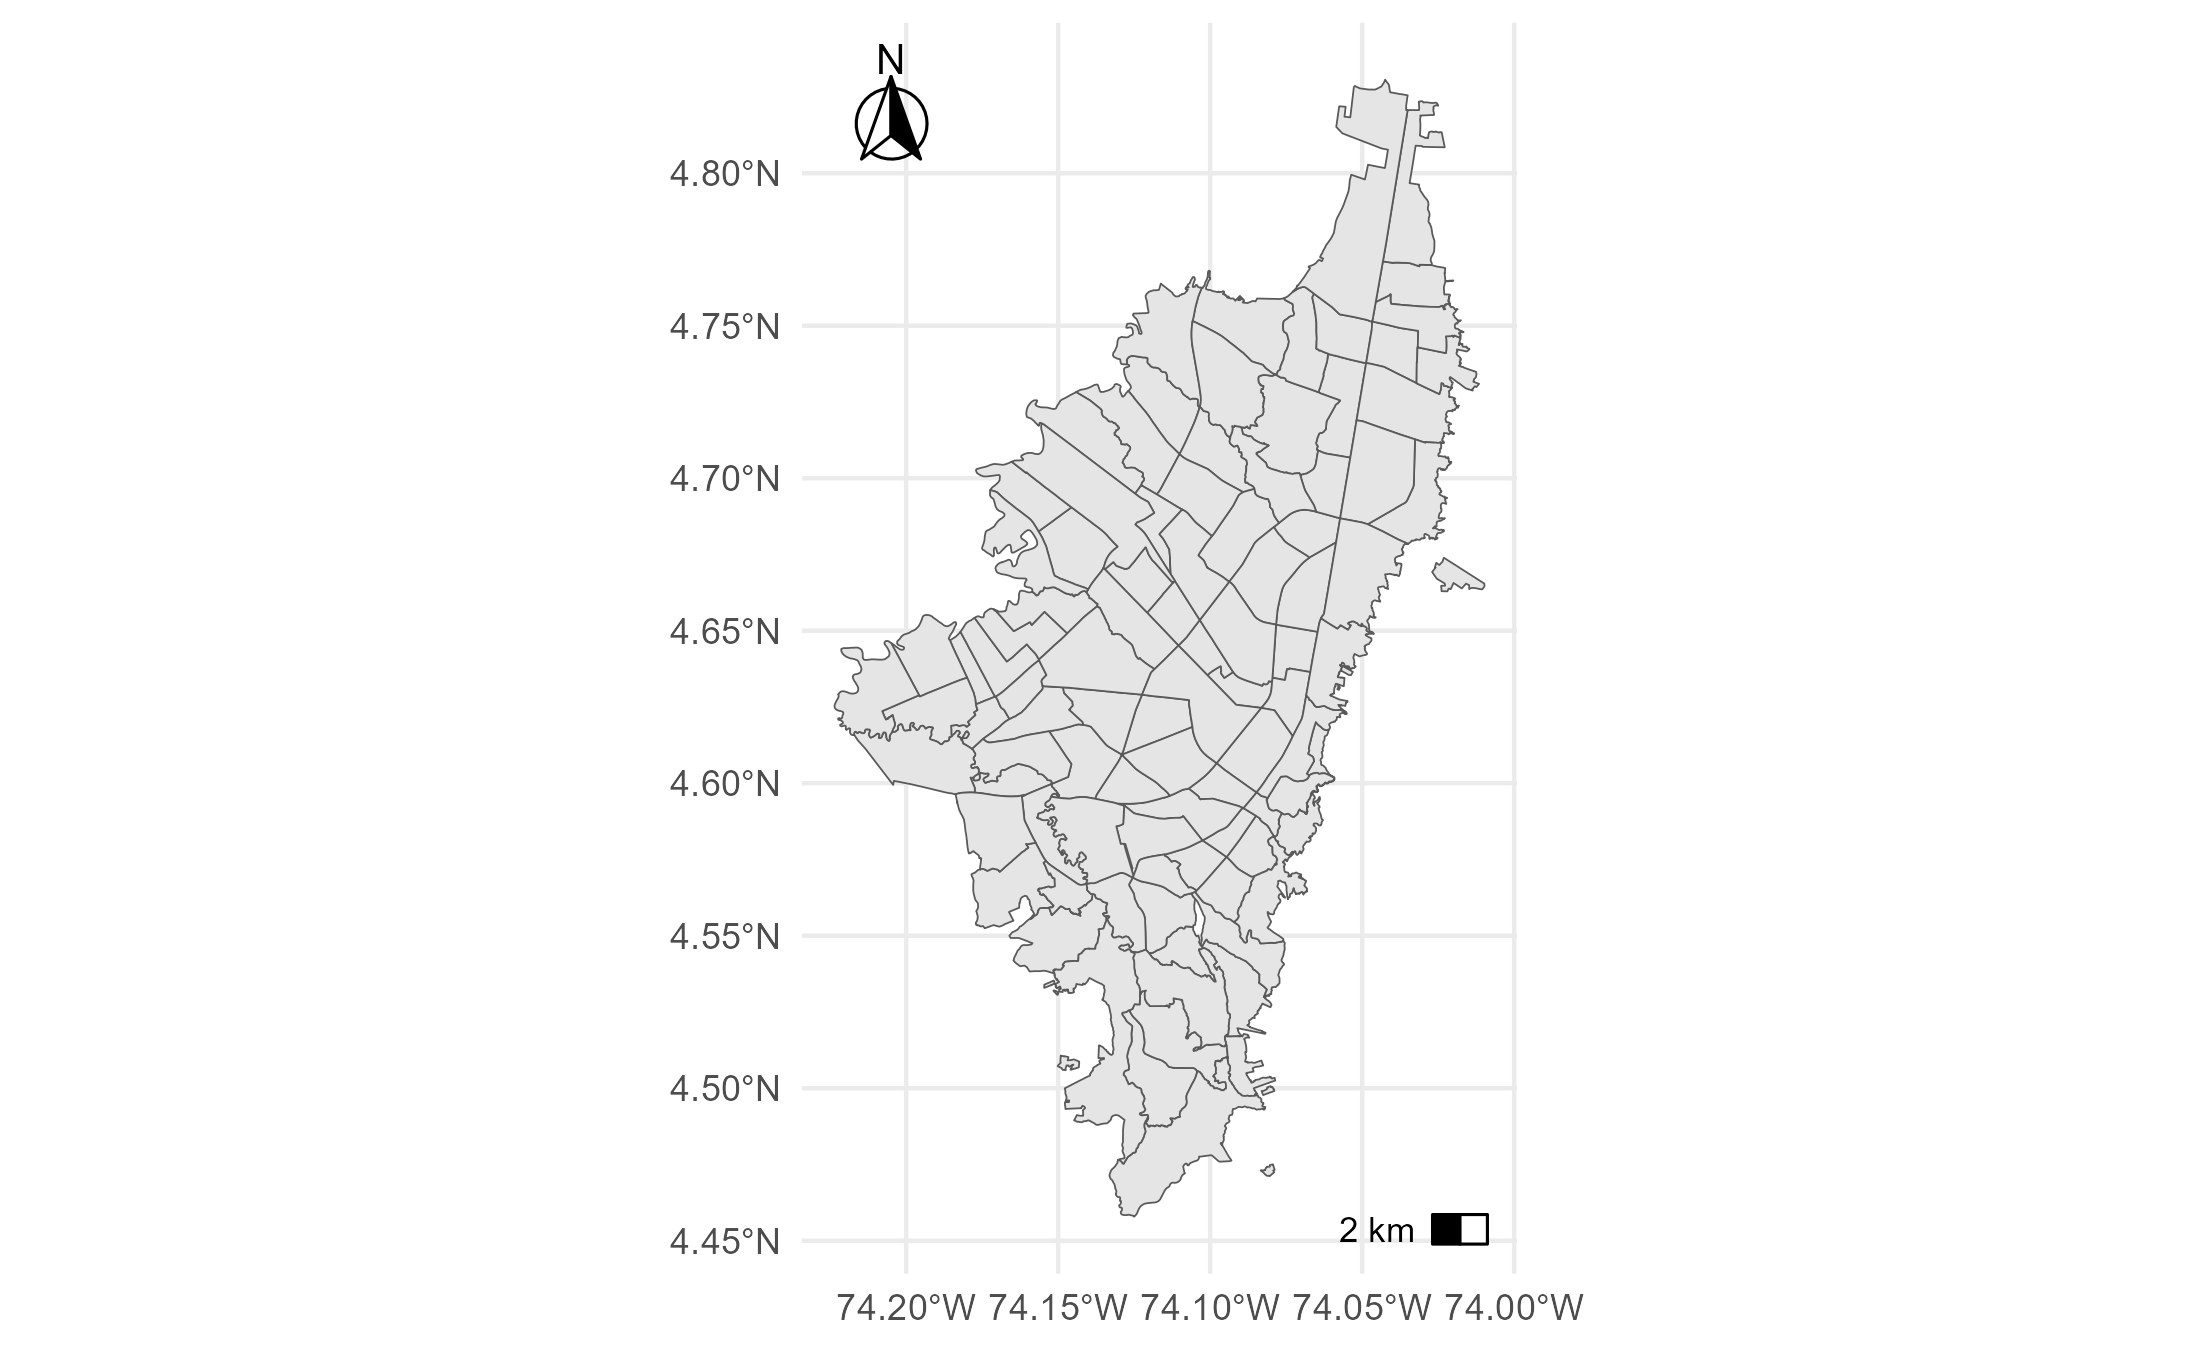
\includegraphics[width=16cm]{Data/Results/Images/Study_Area_UPZ.png}
    \caption{Bogotá boundary with ZPU local limits \citep{ secretariadistritaldeplaneacionCapaGeograficaEncuesta2023}}
    \label{fig:Study_Area_ZPU}
\end{figure}


\section{Spatial analysis unit}

The geographical analysis unit used in this study is a hexagon grid. The hexagon shape of the grid has convenient features when computing measures across different resolution spatial datasets. For example, having an equivalent distance from a hexagon of interest to their corresponding neighbouring hexagons generates more accurate time and distance operations between cells \citep{ubertechnologiesH3HexagonalHierarchical2023}. For example, Figure \ref{fig:Hex_grid_example} shows how a hexagon shape grid can aggregate spatial data, regardless of the features underlying geometries or boundaries of the spatial analysis units from the initial dataset. The spatial resolution of the grid used in this study has a level 9, representing an average area of 0.105 square kilometres \citep{ubertechnologiesH3HexagonalHierarchical2023}.

\begin{figure}[H]
    \centering
    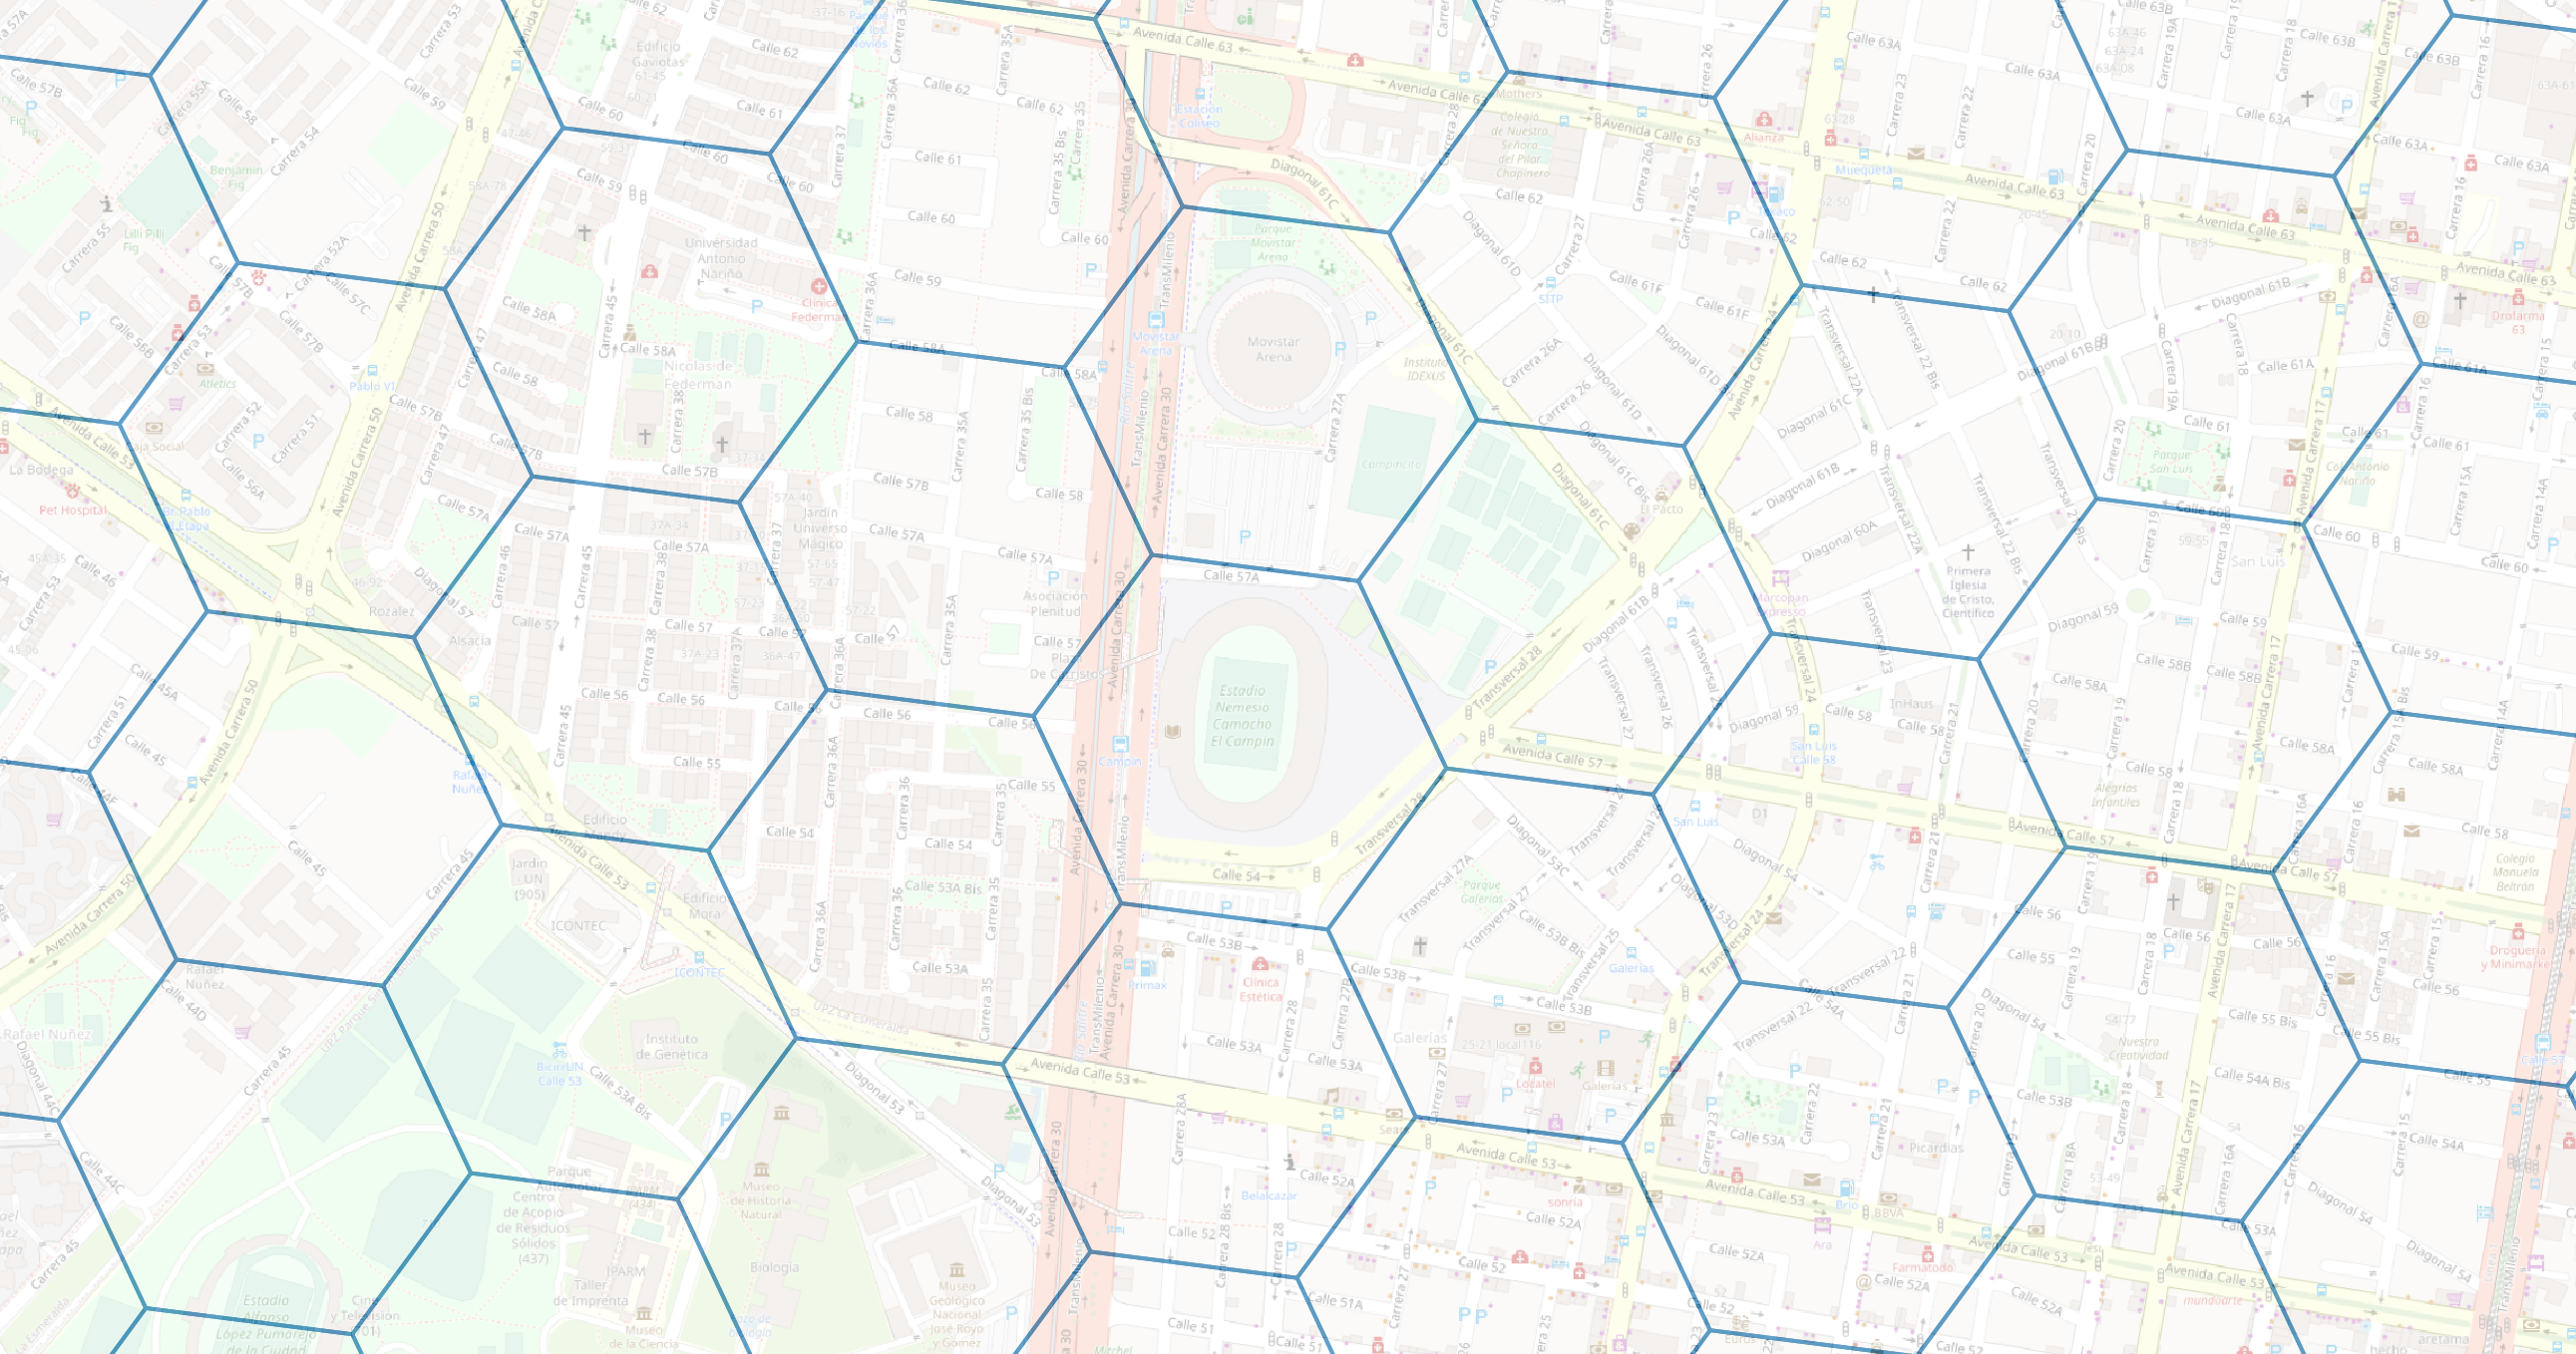
\includegraphics[width=10cm]{Images/Hex_grid.png}
    \caption{Resolution 9 hexagon grid example in Bogotá \citep{openstreetmapcontributorsPlanetDumpRetrieved2023a}}
    \label{fig:Hex_grid_example}
\end{figure}

\section{Workflow for data preparation}

To correctly model accessibility, transport infrastructure data, land use data and demographic data should be all combined in the same framework, as they are the main elements influencing urban accessibility \citep{pereiraIntroductionUrbanAccessibility2023a}. Figure \ref{fig:Workflow_Summary} summarises the preprocessing workflow to transform the input data into the appropriate format data for the accessibility modelling. As described in Table \ref{tab:Data_summary}, the BRT data, the street network and the metro data will comprise the transport infrastructure component, while the land use data and the survey data will form the land use and demographic component, respectively.

\begin{figure}[H]
    \centering
    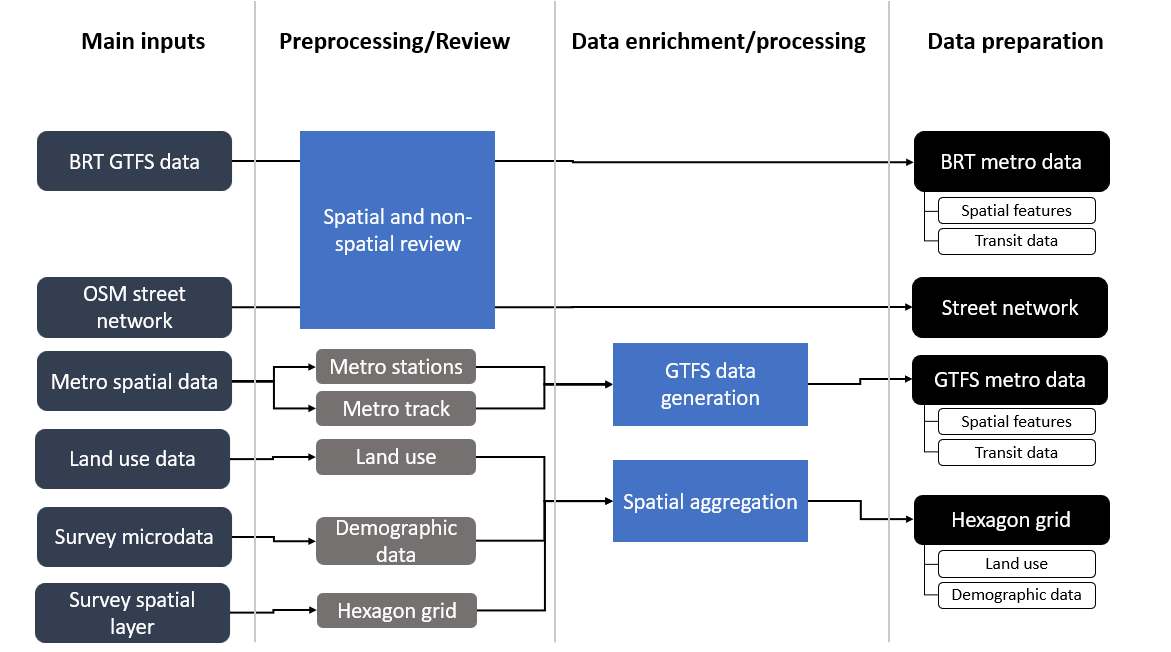
\includegraphics[width=13cm]{Images/Workflow_summary.png}
    \caption{Workflow summary diagram}
    \label{fig:Workflow_Summary}
\end{figure}

\section{GTFS data generation}

As this research aims to assess the accessibility impact of the future metro operation, the modelling process requires combining both modes of transportation in the same modelling exercise. Although the metro system is not yet operational, the metro transit data must be generated to be considered an available mode in the modelling process. Therefore, the metro transit information must be created with information about the infrastructure and the transit service published by the local authorities.

The current BRT transit information is already published in GTFS format by \citep{alcaldiadebogotad.c.EstacionesPrimeraLinea2022,alcaldiadebogotad.c.TrazadoPrimeraLinea2022} and previous reference of GTFS data for multimode transport modelling exercises \citep{pereiraIntroductionUrbanAccessibility2023a}, the metro transit data must be structured in GTFS format. The next subsections highlight the main spatial and alphanumeric procedures to generate the man tables of the GTFS data for future metro transit operations, as presented in Figure \ref{fig:GTFS_structure}.

The structuring and generation of the GTFS table were made considering the official GTFS specification \citep{mobiltydataGeneralTransitFeed2023} and the previous application made by \cite{pereiraIntroductionUrbanAccessibility2023a}.

\subsection{Agency}

The agency table in the GTFS data structure contains general information on the provider entity of the transit services. As Bogotá Metro company already exists, the agency table contains their already known information.


\begin{table}[ht]
\centering
\renewcommand{\arraystretch}{1.5}
\resizebox{\textwidth}{!}{%
\centering
\begin{tabular}{llllll}
  \hline
  agency\_id & agency\_name & agency\_url & agency\_timezone & agency\_lang & agency\_phone \\ 
  \hline
  1 & Metro de Bogota & https://www.metrodebogota.gov.co/ & America/Bogota & es & (+57)601-555-33-33 \\ 
  \hline
\end{tabular}}
\caption{Metro agency table.}
\label{tab:Metro_Agency}
\end{table}

\subsection{Routes}

The scope of the current metro construction project includes the metro infrastructure for the first line, and so does the scope of this research. The track of the metro line draws a north-south line in the east zone of Bogotá to further go to the southwest of the city, as shown in Figure \ref{fig:Metro_Network} . For modelling purposes, this research will consider two possible routes:

\begin{itemize}
\item South route: The southern route will begin in the station located further southwest of the city and finish in the station located further north.
\item North route: The northern route will start at the further north located station and end at the station further southwest in Bogotá.
\end{itemize}

\begin{table}[ht]
\centering
\renewcommand{\arraystretch}{1.5}
\resizebox{\textwidth}{!}{%
\begin{tabular}{llllllll}  % <--- Changed column specification, removed "r"
  \hline
  route\_id & route\_short\_name & route\_long\_name & route\_desc & agency\_id & route\_color & route\_text\_color & route\_type \\ 
  \hline
  M1\_001 & S\_001 & South & Main & 1 & FFFFFF & 000000 & 1 \\ 
  M1\_002 & N\_001 & North & Main & 1 & FFFFFF & 000000 & 1 \\ 
  \hline
\end{tabular}}
\caption{Metro routes table.}
\label{tab:Metro_Routes}
\end{table}

As shown in Table \ref{tab:Metro_Routes}, the route must include the general identification data from each route, together with the provider entity and the mode of transport of the transit service, in the agency\_id and route\_type fields, respectively. The agency\_id field has a "1" value, consequently with the value given with the agency\_id field in \ref{tab:Metro_Agency} to the service provided. In like manner, the value "1" in the route\_type field indicates the mode of transport of the route metro or subway \citep{mobiltydataGeneralTransitFeed2023}. 

\subsection{Trips}

The trips represent the service unit of the transit service. A trip for each route will be considered in the modelling as shown in Table \ref{tab:Metro_Trips}. Apart from the identification data from each trip, the trip data also include a reference to the shape table in the shape\_id field, which will be explained later.


\begin{table}[ht]
\centering
\renewcommand{\arraystretch}{1.5}
%\resizebox{\textwidth}{!}
\caption{Metro trips table.}
\label{tab:Metro_Trips}
\end{table}

\subsection{Calendar and Calendar Dates}

The calendar and calendar date table allow transit planning practitioners to schedule the days of the week when the service of a trip operates and what particular date can be included or omitted from the operation. The scheduling structure of the metro service was based on the published schedule of the current BRT service. Both tables for the metro service are presented in Table \ref{tab:Metro_Calendar} and Table \ref{tab:Metro_Calendar_Dates}, respectively.

\begin{table}[ht]
\centering
\resizebox{\textwidth}{!}{%
\begin{tabular}{lrrrrrrrll}
  \hline
  service\_id & monday & tuesday & wednesday & thursday & friday & saturday & sunday & start\_date & end\_date \\ 
  \hline
  1 &   0 &   0 &   0 &   0 &   0 &   0 &   1 & 20000101 & 20990101 \\ 
  2 &   1 &   1 &   1 &   1 &   1 &   0 &   0 & 20000101 & 20990101 \\ 
  3 &   1 &   1 &   1 &   1 &   1 &   0 &   0 & 20000101 & 20990101 \\ 
  4 &   1 &   1 &   1 &   1 &   1 &   0 &   0 & 20000101 & 20990101 \\ 
  5 &   1 &   1 &   1 &   1 &   1 &   0 &   0 & 20000101 & 20990101 \\ 
  6 &   1 &   1 &   1 &   1 &   1 &   0 &   0 & 20000101 & 20990101 \\ 
  7 &   1 &   1 &   1 &   1 &   1 &   1 &   0 & 20000101 & 20990101 \\ 
   \hline
\end{tabular}}
\caption{Metro calendar table.}
\label{tab:Metro_Calendar}
\end{table}

Using the service\_id field, the calendar table allows establishing different types of service scheduling by weekday in a specific date range. Similarly, the calendar dates table can add or remove a service from a specific date according to the value in the exception\_type field.

\begin{table}[ht]
\centering
%\resizebox{\textwidth}{!}
\caption{Metro calendar date table.}
\label{tab:Metro_Calendar_Dates}
\end{table}

\subsection{Shapes}

The shape table contains the geometry of the path of the trip. As the track path of the future metro has already been published in a spatial format, the shape table data will be structured based on the publicly available geometry of the metro track. As the modelling will be based on the assumption of one trip for each of the north and south routes, the geometry of the trips will only differ in the sequential order in which they travel the path.

Table \ref{tab:Metro_Shapes} shows a preview of the result of converting the spatial data of the track path into the shape table GTFS format. The shapes table contains the longitude and latitude coordinates of the path in the shape\_pt\_lon and shape\_pt\_lat fields, respectively. Equally important, the table indicates the sequential order where the transit service will travel the path with an ascending integer values sequence in the shape\_pt\_sequence field.

\begin{table}[ht]
\centering
\begin{tabular}{lrllr}
  \hline
shape\_id & shape\_dist\_traveled & shape\_pt\_lon & shape\_pt\_lat & shape\_pt\_sequence \\ 
  \hline
M1\_001 & 0.00 & -74.06046 & 4.667379 &   1 \\ 
M1\_001 & 30.15 & -74.06051 & 4.667112 &   2 \\ 
M1\_001 & 30.57 & -74.06051 & 4.667109 &   3 \\ 
M1\_001 & 30.99 & -74.06051 & 4.667105 &   4 \\ 
M1\_001 & 31.42 & -74.06051 & 4.667101 &   5 \\ 
M1\_001 & 31.84 & -74.06051 & 4.667098 &   6 \\ 
   \hline
\end{tabular}
\caption{Metro shapes table.}
\label{tab:Metro_Shapes}
\end{table}

\subsection{Stops}

The stops table in the GTFS data structure stores the location and identification data from the stations where the transport user can begin or end using the metro transportation mode. Again, the stop data is generated based on the locations of stations contained in the spatial station's data public by the Bogotá Metro. After converting from a spatial data structure to a GTFS data structure, Table \ref{tab:Metro_Stops} shows the stops table from the metro GTFS data.

\begin{table}[ht]
\centering
\resizebox{\textwidth}{!}{%
\begin{tabular}{lllllll}
  \hline
stop\_id & stop\_code & stop\_name & stop\_lat & stop\_lon & location\_type & zone\_id \\ 
  \hline
M01 & 01 & Cra 96-01 & 4.640571 & -74.17746 & 0 & 0 \\ 
M02 & 02 & Portal de las Américas-02 & 4.630021 & -74.17186 & 0 & 0 \\ 
M03 & 03 & Carrera 80-03 & 4.622248 & -74.16671 & 0 & 0 \\ 
M04 & 04 & Calle 42 Sur-04 & 4.615737 & -74.16042 & 0 & 0 \\ 
M05 & 05 & Kennedy-05 & 4.617298 & -74.15159 & 0 & 0 \\ 
M06 & 06 & Av Boyaca-06 & 4.618484 & -74.14063 & 0 & 0 \\ 
   \hline
\end{tabular}}
\caption{Metro stops table.}
\label{tab:Metro_Stops}
\end{table}

\subsection{Stop times}

The stops times table indicates the arrival and departure times at every station a trip goes through. Although the local authorities or the metro company have not published specific timetables for future trips, the general scheduling and time between stations can be inferred from the available data.

The metro company, jointly with Bogotá's city council, have stated that the metro line will travel at an average speed of 43 km/h, allowing the Bogotá population to travel from the station on the south edge of the line to the last station on the opposite north edge in 27 minutes \citep{metrodebogotaPrimeraLineaMetro2022}. After calculating the distance between the stations' locations and the average travel speed of the metro, it is possible to establish the estimated arrival and departure time at every station for every trip. As the trips differ in the order they go through the stations, the data generation process is essentially the same but sequentially inverted. Table \ref{tab:Metro_Stop_Times} shows an overview of the stop times table of a trip from the north route, coupled with the stop\_sequence field that indicates the order of the stations.


\begin{table}[ht]
\centering
\resizebox{\textwidth}{!}{%
\begin{tabular}{llllrr} % Removed the "r" column specifier
  \hline
  trip\_id & arrival\_time & departure\_time & stop\_id & stop\_sequence & timepoint \\ 
  \hline
  M1\_002\_N\_3\_M1\_002 & 08:00:00 & 08:00:00 & M01 & 1 & 0 \\ 
  M1\_002\_N\_3\_M1\_002 & 08:01:52 & 08:01:52 & M02 & 2 & 0 \\ 
  M1\_002\_N\_3\_M1\_002 & 08:03:19 & 08:03:19 & M03 & 3 & 0 \\ 
  M1\_002\_N\_3\_M1\_002 & 08:04:44 & 08:04:44 & M04 & 4 & 0 \\ 
  M1\_002\_N\_3\_M1\_002 & 08:06:08 & 08:06:08 & M05 & 5 & 0 \\ 
  \hline
\end{tabular}}
\caption{Metro stop times table.}
\label{tab:Metro_Stop_Times}
\end{table}

It is important to realize that the arrival and departure times listed in Table \ref{tab:Metro_Stop_Times} assume that the transit user would be aboard instantly. Although unrealistic, this was kept intentionally in this matter. After reviewing the BRT GTFS data \citep{transmilenios.a.GTFSEstaticos202306212023}, all BRT transit's arrival and departure times presented the same behaviour. Hence, for modelling proposes, the resulting metro GTFS data will reflect this similarly to prevent artificially affecting the competitiveness between modes.

\subsection{Frequencies}

The frequencies table accounts for how often the trips depart from their respective first station during the day. The frequency of travel will vary depending on the current commuting temporal patterns in Bogotá. According to \cite{alcaldiadebogotad.c.EncuestaMovilidad20192019}, the schedule will assume a peak hour between 5:30 and 9:00 a.m. and 4:00 and 7:00 p.m. During the peak and non-peak hours, the frequencies of the trips will be one every 3 minutes and one every 15 minutes, respectively. The seconds' values in the headwat\_secs field express the hourly differentiated schedule for the time ranges established in the start\_time and end\_time fields.

\begin{table}[ht]
\centering
\begin{tabular}{llllrr} % Removed the "r" column specifier
  \hline
  trip\_id & start\_time & end\_time & headway\_secs & exact\_times \\ 
  \hline
  M1\_001\_S\_3\_M1\_001 & 00:00:00 & 05:29:59 & 900 & 0 \\ 
  M1\_001\_S\_3\_M1\_001 & 05:30:00 & 08:59:59 & 180 & 0 \\ 
  M1\_001\_S\_3\_M1\_001 & 09:00:00 & 15:59:59 & 900 & 0 \\ 
  M1\_001\_S\_3\_M1\_001 & 16:00:00 & 18:59:59 & 180 & 0 \\ 
  M1\_001\_S\_3\_M1\_001 & 19:00:00 & 23:59:59 & 900 & 0 \\ 
  \hline
\end{tabular}
\caption{Metro frequencies table.}
\label{tab:Metro_Frequencies}
\end{table}


\section{Spatial aggregation}

% Refence to the hexagon grid

The study uses a hexagon grid as a common spatial observation unit for both the inputs and results of the accessibility modelling process. With the spatial land use information, the location of opportunities can be geographically represented using the hexagon according to the activity related to a land use category of interest. Similarly, the demographic data available can describe socioeconomic and living conditions features of the inhabitant's location in a given hexagon grid.

\subsection{Land use}


The land use data published by \cite{alcaldiadebogotad.c.DestinoEconomicoPredominante2022} is a spatial shapefile format containing the registered perimeter boundary of all terrains. Each feature represented the geometry of the terrain, and the land use category was stored in a character column in the spatial data set.

To aggregate land use data to the hexagon grid, the intersecting geometries of every terrain were counted and grouped by their respective land use case to count for the number of each land use terrain location within each hexagon grid. Henceforth, the resulting grid contained the terrain for every land use category. As the hexagon grid has a homogeneous area, the results can be interpreted as the terrain density by hexagon for the land use category of interest. Figure \ref{fig:Opportunities_Spatial} presents the resulting hexagon grid for the commercial corridor land use density.

\begin{figure}[H]
    \centering
    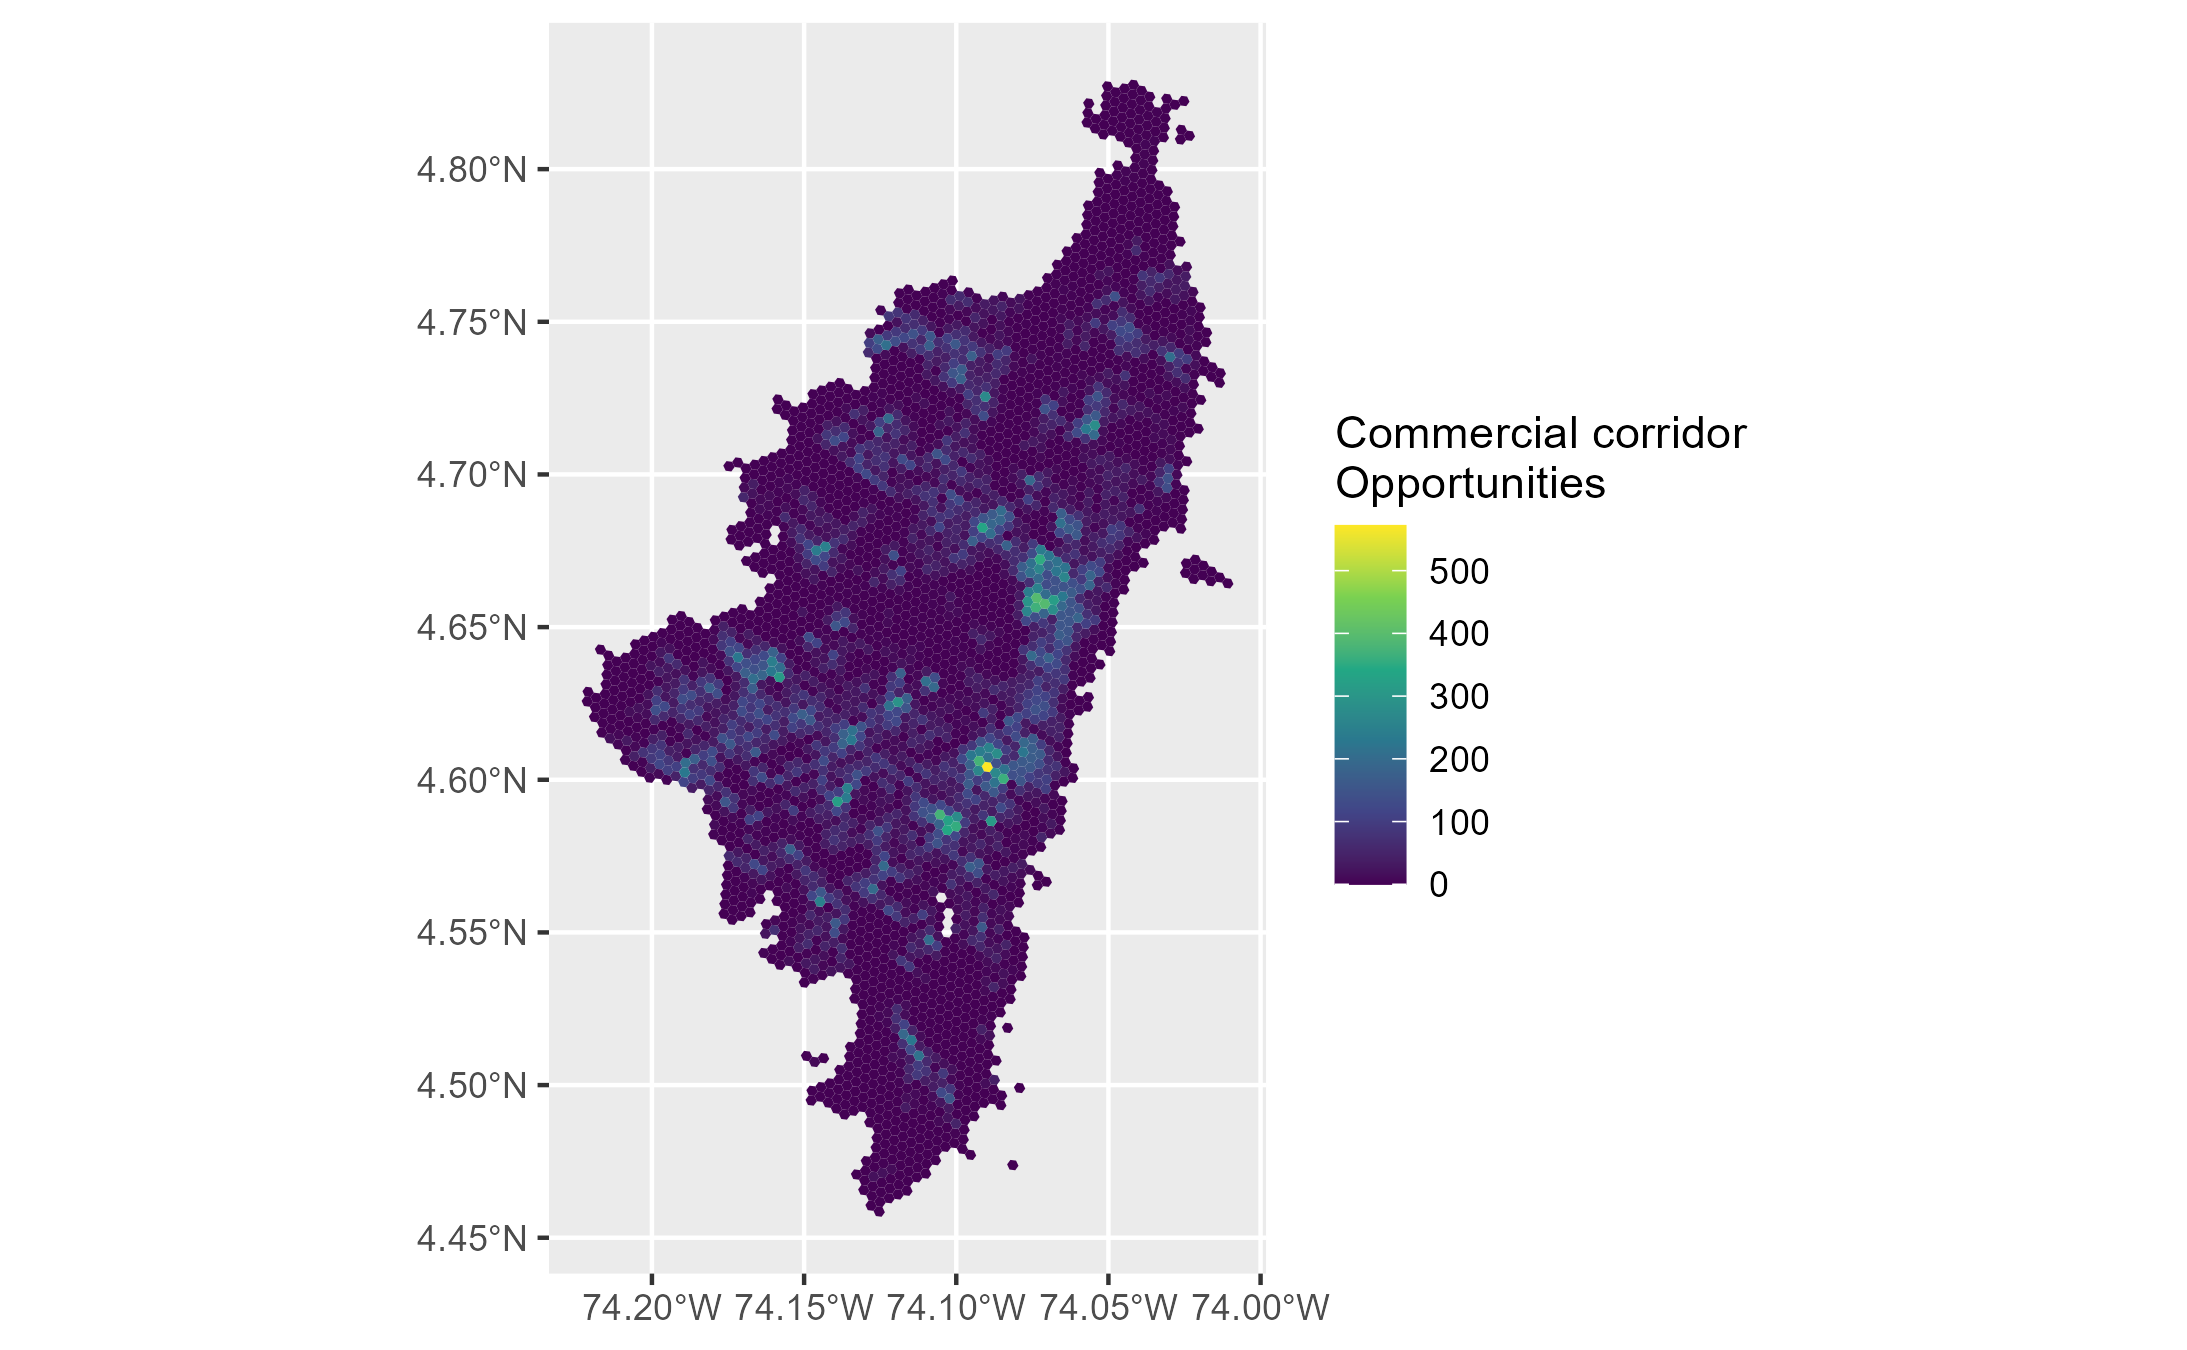
\includegraphics[width=13cm]{Data/Results/Images/Opportunities_COD_21.png}
    \caption{Spatial commercial corridor land use density}
    \label{fig:Opportunities_Spatial}
\end{figure}


\subsection{Demographics} \label{Demographics}

The aggregation of demographic data to the hexagon would allow the assessment of socioeconomic variables of Bogotá's inhabitants across space. This study will incorporate income data gathered by \cite{secretariadistritaldeplaneacionMicrodatosEncuestaMultiproposito2023} to the hexagon grid.

The income data used in this study was initially in a non-spatial format. First, it was grouped and georeferenced using the ZPU that \cite{secretariadistritaldeplaneacionMicrodatosEncuestaMultiproposito2023} provided. Second, the household average income was calculated considering the a household could have multiple members that generate income. Third, the overall ZPU income average vas calculated and integrated with the corresponding ZPU spatial layer. Finally, the mean hexagon income was computed using an area-weighted average. As the boundaries of the ZPU are disparate and uneven, the income value computed for the hexagon results from a weighted average using the income value of each ZPU and the percentage or intersection area of each ZPU, respectively. 

Figure \ref{fig:Income_Decile_Hex} shows the resulting hexagon grid after the spatial aggregation and after grouping the hexagons by income deciles.

\begin{figure}[H]
    \centering
    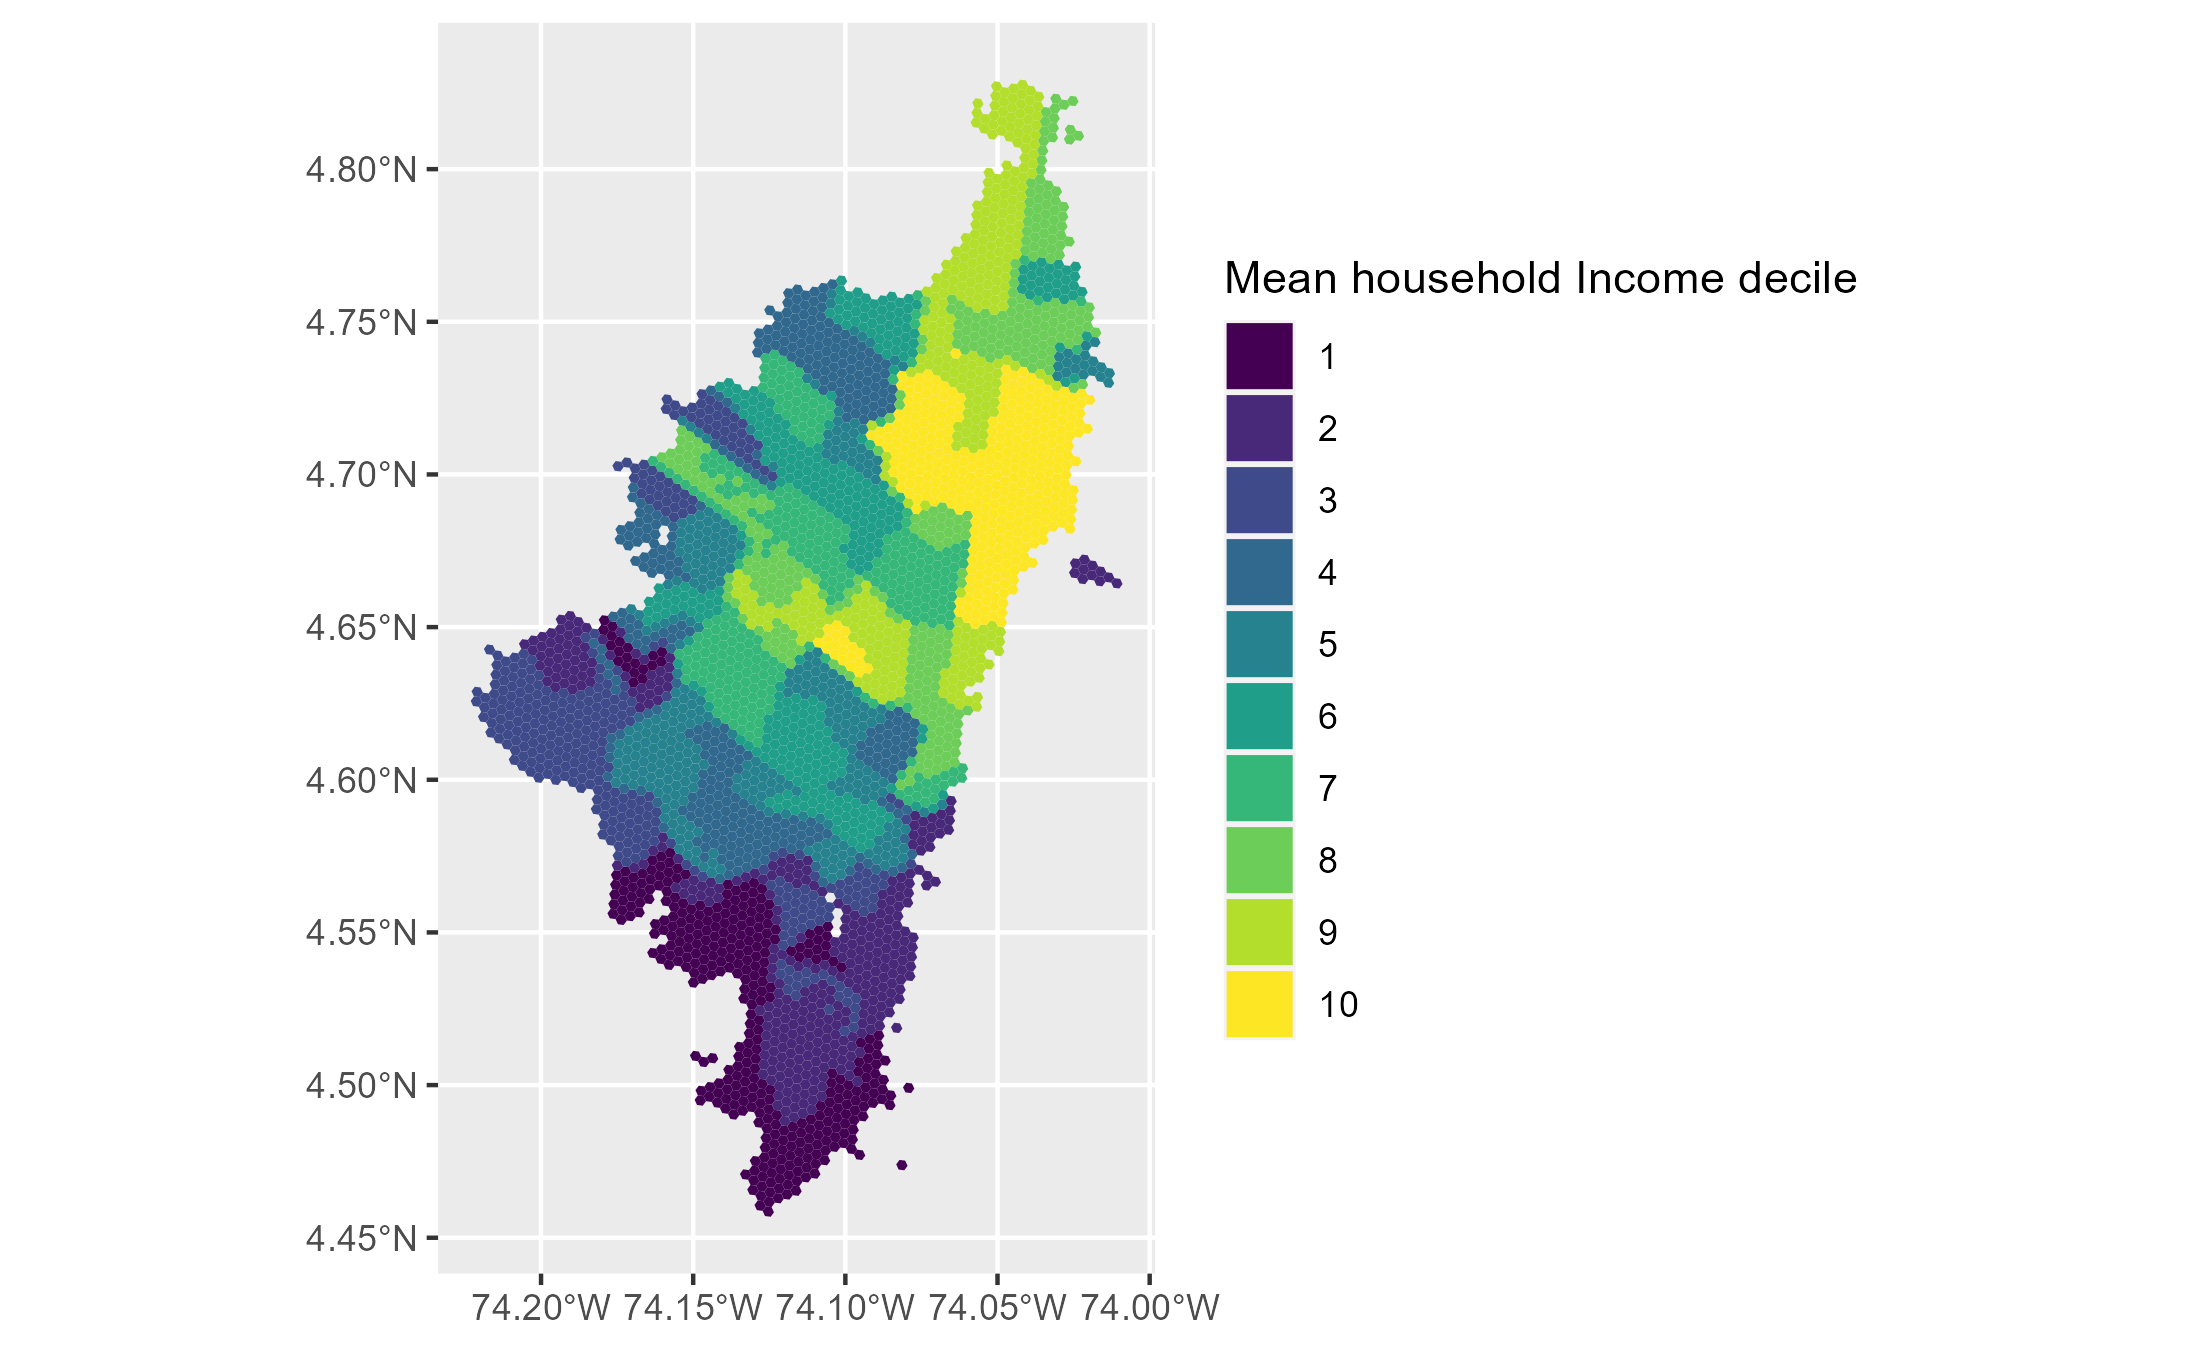
\includegraphics[width=13cm]{Data/Results/Images/Demo_income_decile_discrete.png}
    \caption{Resulting hexagon grid average household income decile}
    \label{fig:Income_Decile_Hex}
\end{figure}


\section{Accessibility measure}

The accessibility measure chosen to model is a cumulative active accessibility measure. The cumulative accessibility measure accounts for the number of opportunities a person can reach from a given origin location without surpassing the predefined threshold. In other, word cumulative accessibility measures how many opportunities a person can access given their location, the opportunities for spatial distribution and the transit operation.

According to \cite{pereiraIntroductionUrbanAccessibility2023a}, the cumulative accessibility measure can be fine as follows:

\[A_{i}=\sum_{j=1}^{n} O_{j} \times f(c_{ij})\]

\[f(c_{ij})=\begin{cases}
1, & \text{if $c_{ij}$ < $C$}.\\
0, & \text{Otherwise}.
  \end{cases}
\]

where

\begin{itemize}
    \item $A_{i}$ in the accessibility at origin location $i$.
    \item $O_{j}$ is the number of opportunities located at destination $j$.
    \item $n$ is the total number of destinations.
    \item $f(c_{ij})$ is a function that takes 0 or 1 values if the travel cost $c_{ij}$ value from origin $i$ to destination $j$ has exceeded the $C$ travel cost limit. 
\end{itemize}


\section{Scenarios} \label{Scenarios}

This study examined the current and future accessibility scenarios as presented in Figure \ref{fig:Method_Summary}. On the one hand, the current scenario consists of the current transit operation and infrastructure composed of the BRT and street networks. On the other hand, the future scenario will include the BRT and street network, together with the future transit operation and infrastructure for the metro.

It is important to notice that the walking mode is included in all scenarios, and the street network was used to have infrastructure through which the modelling could compute travel by walking. It does not consider any other type of motorized transportation use apart from the BRT network. Additionally, single-mode scenarios were also considered in the accessibility modelling. For control purposes, accessibility for BRT, metro and walking modes was calculated individually to assess accessibility in a disaggregated manner.

\section{Accessibility modelling}

The cumulative accessibility modelling was calculated using the R5R library \citep{pereiraR5rRapidRealistic2021} with R Programming Language. The library calculates accessibility by performing four main procedures. Next, each procedure is described, indicating the inputs required for each one:

\begin{enumerate}
    \item Building multi-mode network: Based on the GTFS data and the street network, a multi-transport mode connects origins and destinations according to the available infrastructure.
    \item Time travel matrix computation: The travel time between all origin and destination combinations is computed, favouring the fastest mode combination available.
    \item Apply cost travel thresholds: According to the threshold parameters, the destination locations are filtered so the accessibility results account for only the destination within the travel cost limits.
    \item Accessibility measure computation: After selecting the destination locations that comply with the travel cost limits, the library uses the land use data and computes the number of reachable opportunities from each origin location within the established limits. 
\end{enumerate}



\subsection{Inputs} \label{Inputs}

The input data provided for each scenario should be aligned with the transit and infrastructure each scenario aims to model. Table \ref{tab:Inputs_By_Scenario} indicates with a check mark the inputs considered for the before and after scenarios as described in \ref{fig:Method_Summary}, together with the additional control scenarios stated in subsection \ref{Scenarios}.


\begin{table}[H]
\centering
\begin{tabular}{c|ccc}
\hline
\multicolumn{1}{l|}{} & \multicolumn{3}{c}{\textbf{Inputs}}                                                   \\ \hline
\textbf{Scenario}     & \multicolumn{1}{l}{\textbf{Street network}} & \textbf{BRT GTFS} & \textbf{Metro GTFS} \\ \hline
Current         & \checkmark & \checkmark &       \\ \hline
Future          & \checkmark & \checkmark & \checkmark \\ \hline
Walking only    & \checkmark &       &       \\ \hline
Metro + walking & \checkmark &       & \checkmark \\ \hline
\end{tabular}
\caption{Input data by scenario.}
\label{tab:Inputs_By_Scenario}
\end{table}

\subsection{Parameters}

% Reference to the threshold

The parameters of the accessibility modelling procedure allow configuring the transit and commuting conditions considered in the urban accessibility computation. The conditions that the R5R parameters can simulate in the accessibility modelling are the maximum walking duration and total commuting duration. Considering the average travel times when using one motorized transit mode in Bogotá \citep{alcaldiadebogotad.c.EncuestaMovilidad20192019}, the maximum walking time and total trip duration had values of 30 and 60 minutes, respectively.

\chapter{Results} \label{Chap5}

\section{Accessibility by scenario}

The accessibility results show the number of reachable opportunities within a travel cost threshold from every possible origin location. The measure was calculated by every scenario described in sections \ref{Scenarios} and \ref{Inputs}, where the scenarios and inputs for the modelling were defined, respectively.



Figure \ref{fig:Results_Opportunities} shows the spatial distribution of opportunities in Bogotá. The accessibility measure accounts for the number of these opportunities from a given location in space that can be reached according to the mode or modes of transportation considered in every scenario. Commercial corridor-related opportunities are spread in the city's west, southwest, east and northeast parts. However, the opportunities appeared clustered in the city's east and northeast parts.



\begin{figure}[H]
    \centering
    \begin{minipage}{0.45\textwidth}
        \centering
        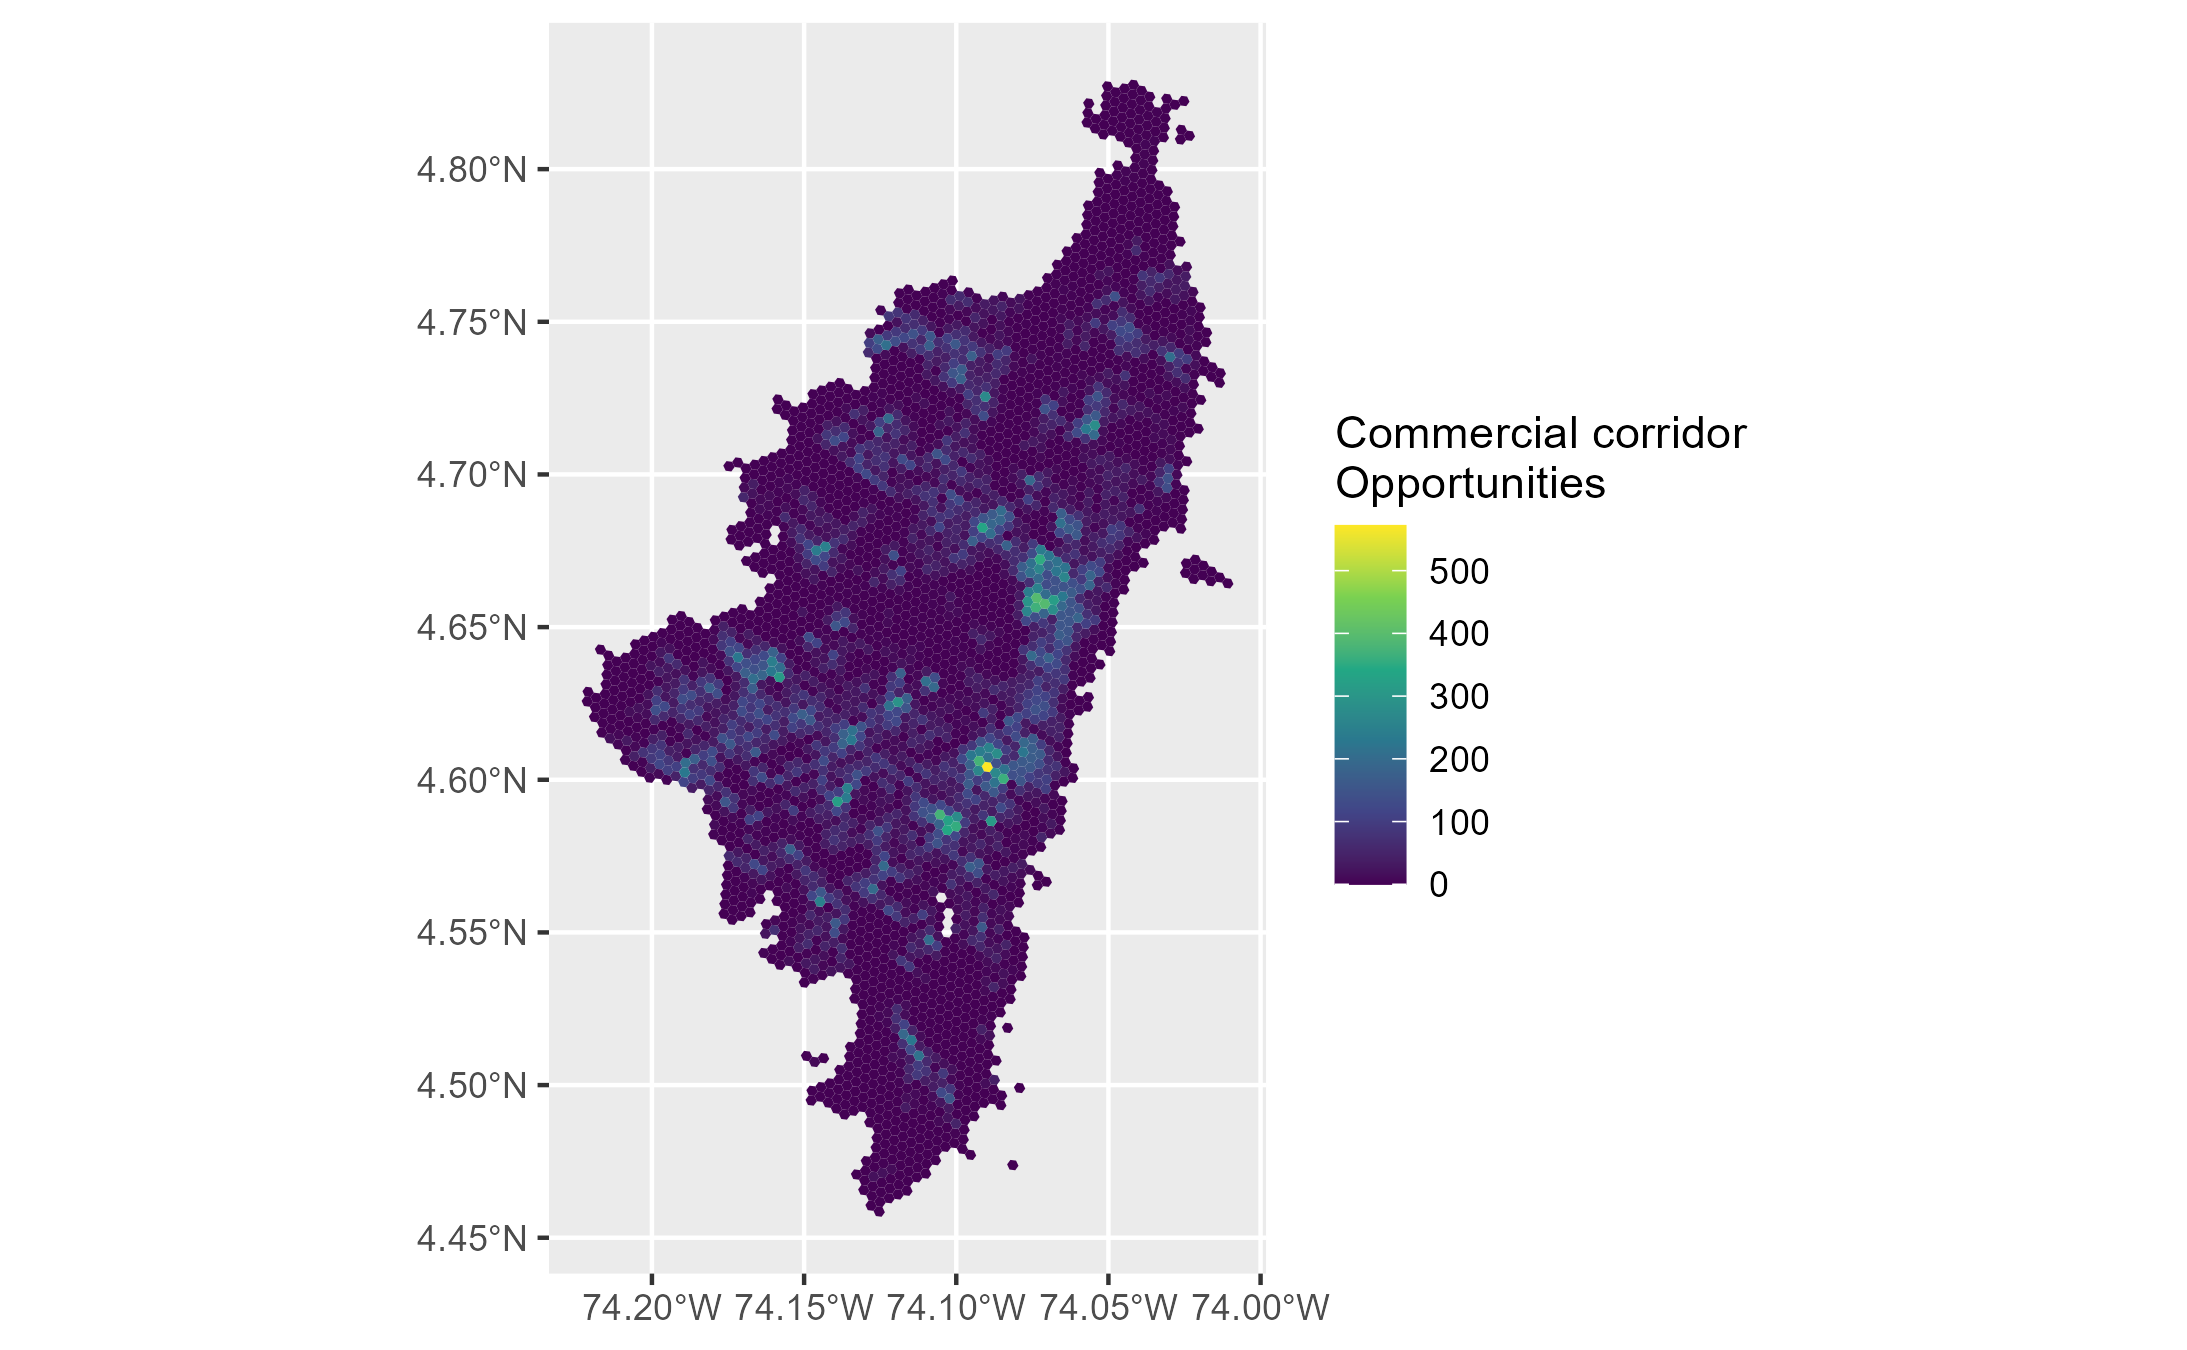
\includegraphics[width=1.3\linewidth]{Data/Results/Images/Opportunities_COD_21.png}
         \caption{Opportunities}
        \label{fig:Results_Opportunities}
    \end{minipage}%
    \hfill
    \begin{minipage}{0.45\textwidth}
        \centering
        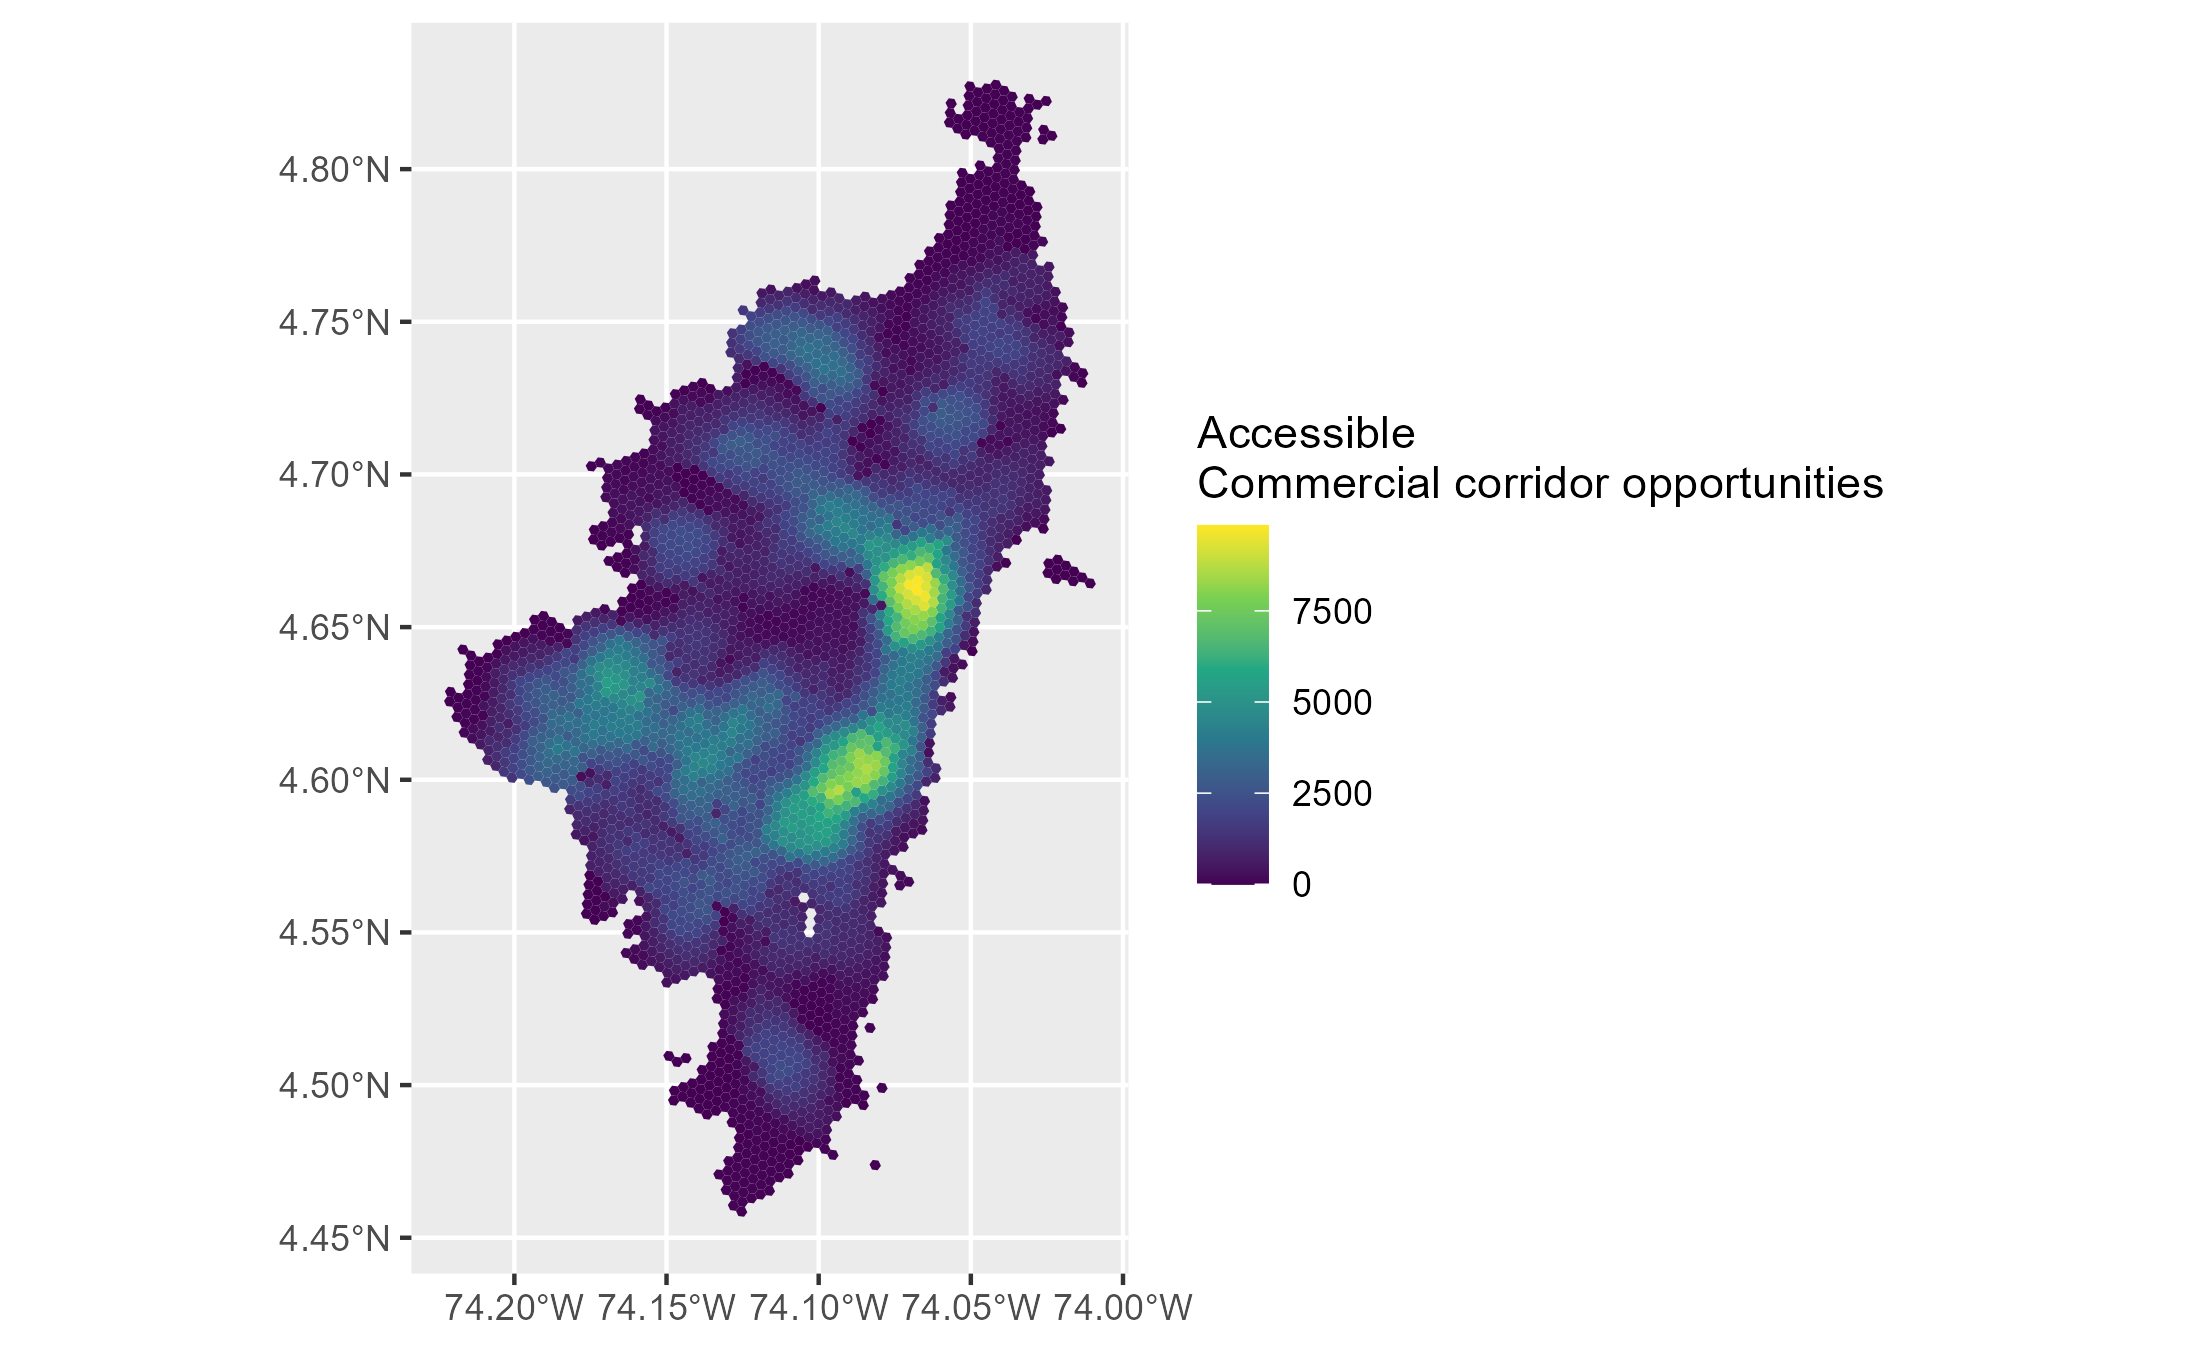
\includegraphics[width=1.3\linewidth]{Data/Results/Images/Access_Walk_base.png}
        \caption{Walking}
        \label{fig:Results_Walking}
    \end{minipage}
\end{figure}

The accessibility results for the walking scenario presented in Figure \ref{fig:Results_Walking} showed the number of reachable opportunities from each location within a 30-minute walking threshold. The walking accessibility results map how the locations located near the major opportunity clusters have higher levels of accessibility compared with locations further away from the opportunity clusters. Consistently with the biggest opportunity clusters, the locations with the higher accessibility values are located in the east and southeast parts of the city.

The process recreates the current scenario's transit condition once the BRT transit operation is included in the modelling inputs. Figure \ref{fig:Access_BRT_Base} presents the accessibility results when enabling the walking and BRT modes. The results show how the BRT transit operation contributes favourably to increasing the accessibility of locations across the city. The locations with high accessibility values in the just walking scenario are no longer those with the highest accessibility values. Due to the BRT transit operation, new locations can reach more opportunities within the same 30-minute walking threshold and the 60-minute total duration limit. Although the commuting conditions in the current modelled scenario do not consider additional modes like bicycles or privately owned cars, it simulates the current commuting situation of 36\% of daily commutes \citep{alcaldiadebogotad.c.EncuestaMovilidad20192019}.

To disaggregate the metro accessibility impact, the results for only metro scenario were modelled. Figure \ref{fig:Results_Metro_Base} shows the accessibility result as a footprint of the route of the future metro line. As the walking mode is included in all scenarios, the accessibility increase is higher in the locations near the stations. The effect smoothly decreases as the walking commuting increases until it no longer complies with the duration thresholds.



\begin{figure}[H]
    \centering
    \begin{minipage}{0.45\textwidth}
        \centering
        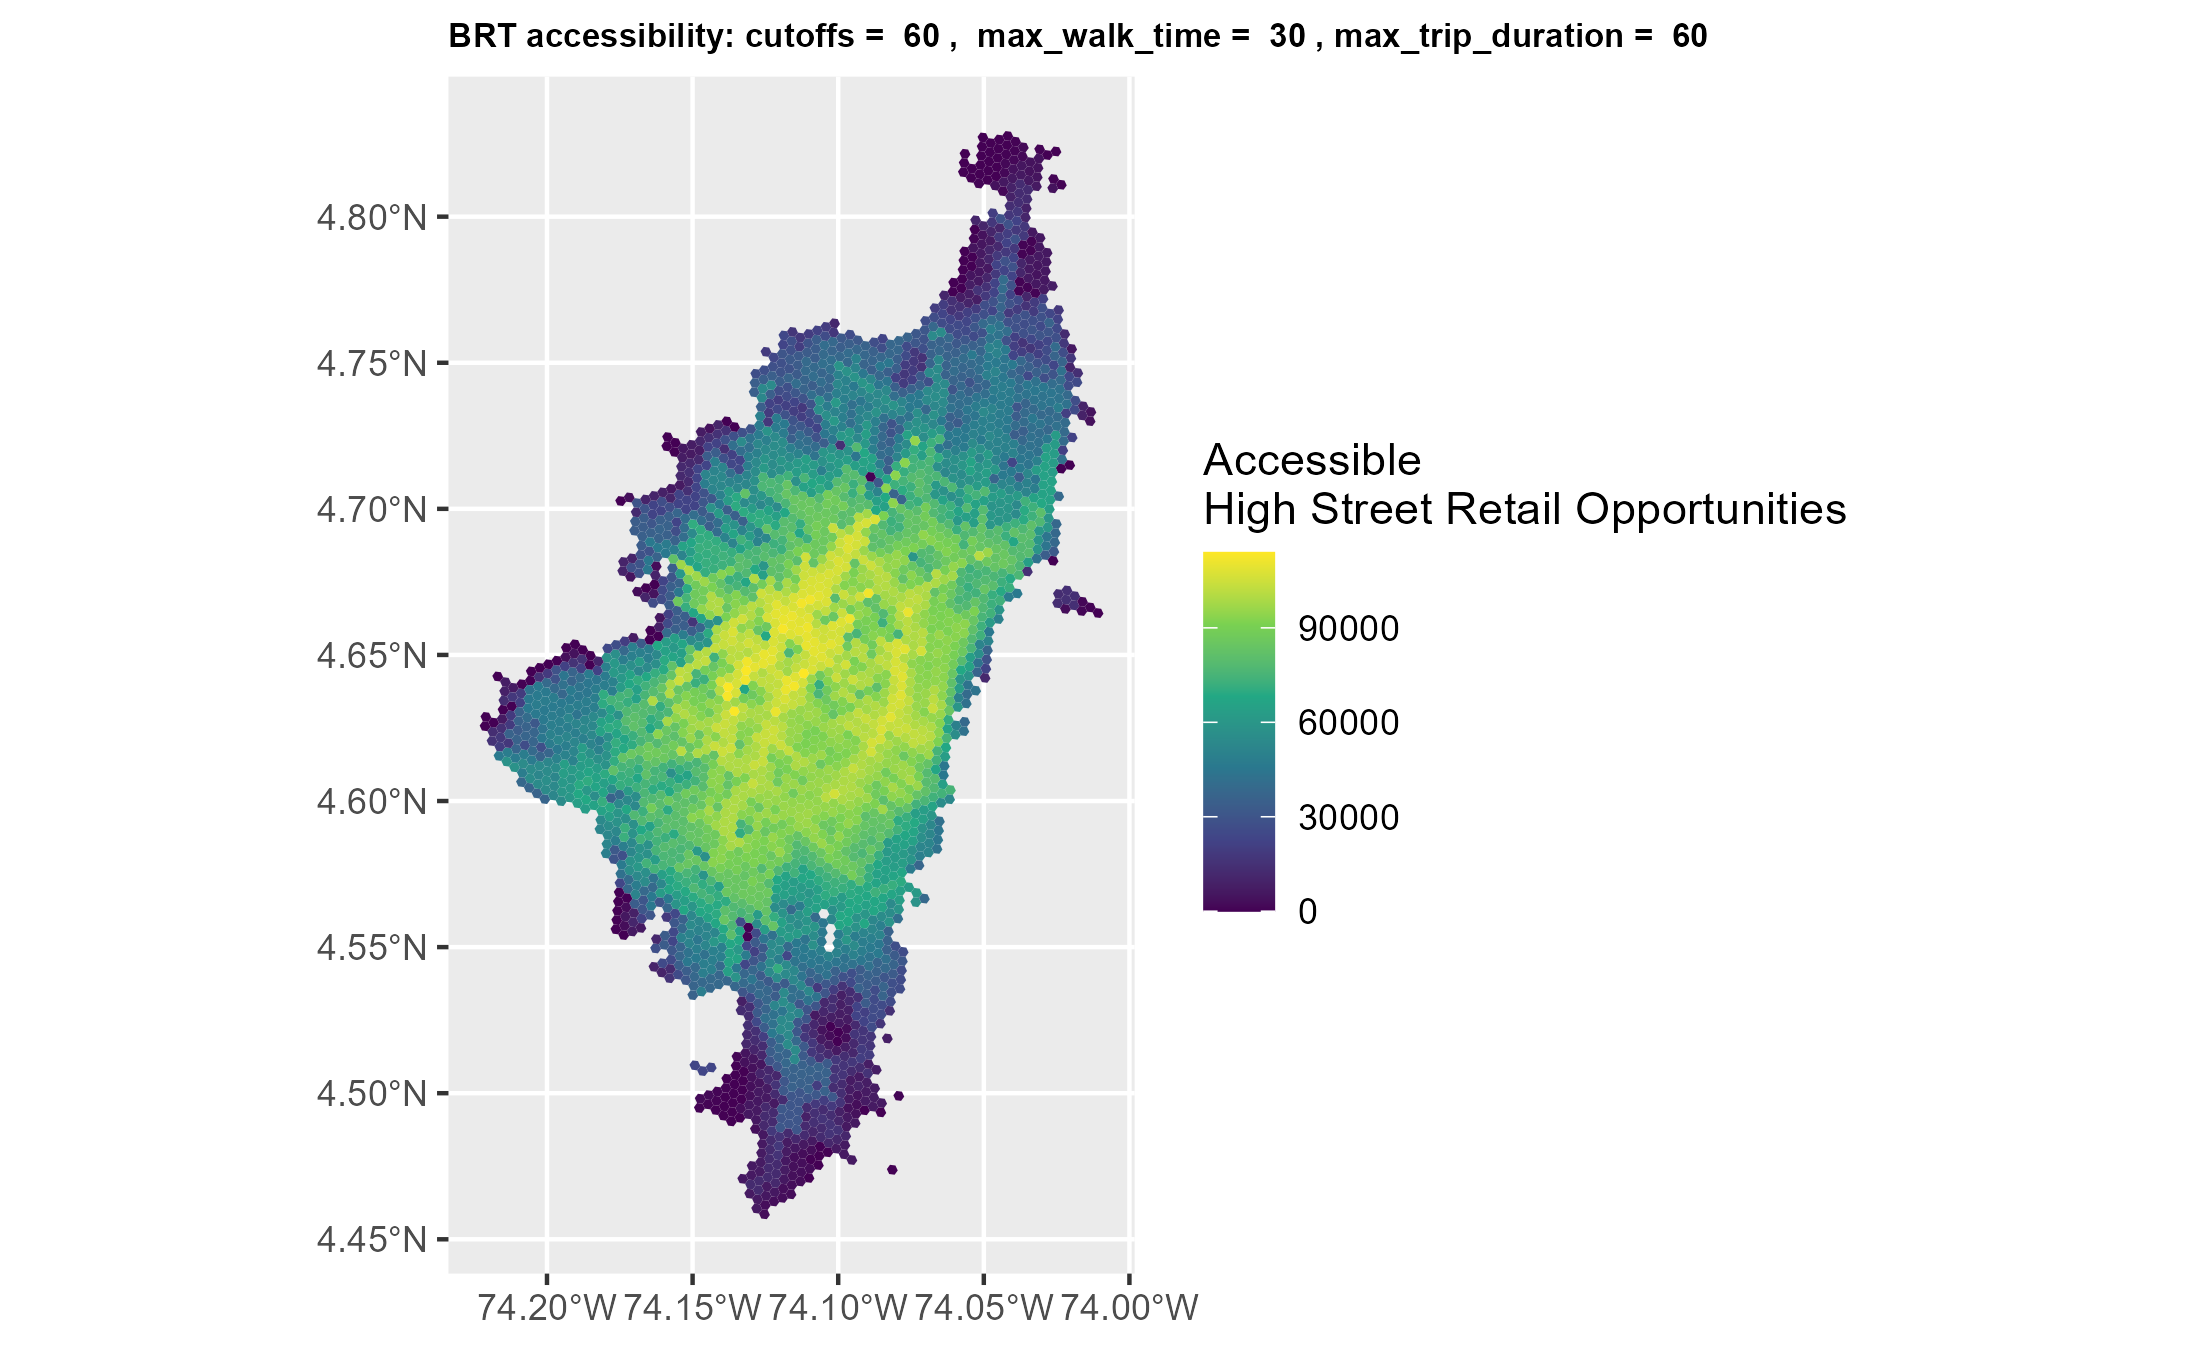
\includegraphics[width=1.3\linewidth]{Data/Results/Images/Access_BRT_base.png}
         \caption{BRT}
        \label{fig:Access_BRT_Base}
    \end{minipage}%
    \hfill
    \begin{minipage}{0.45\textwidth}
        \centering
        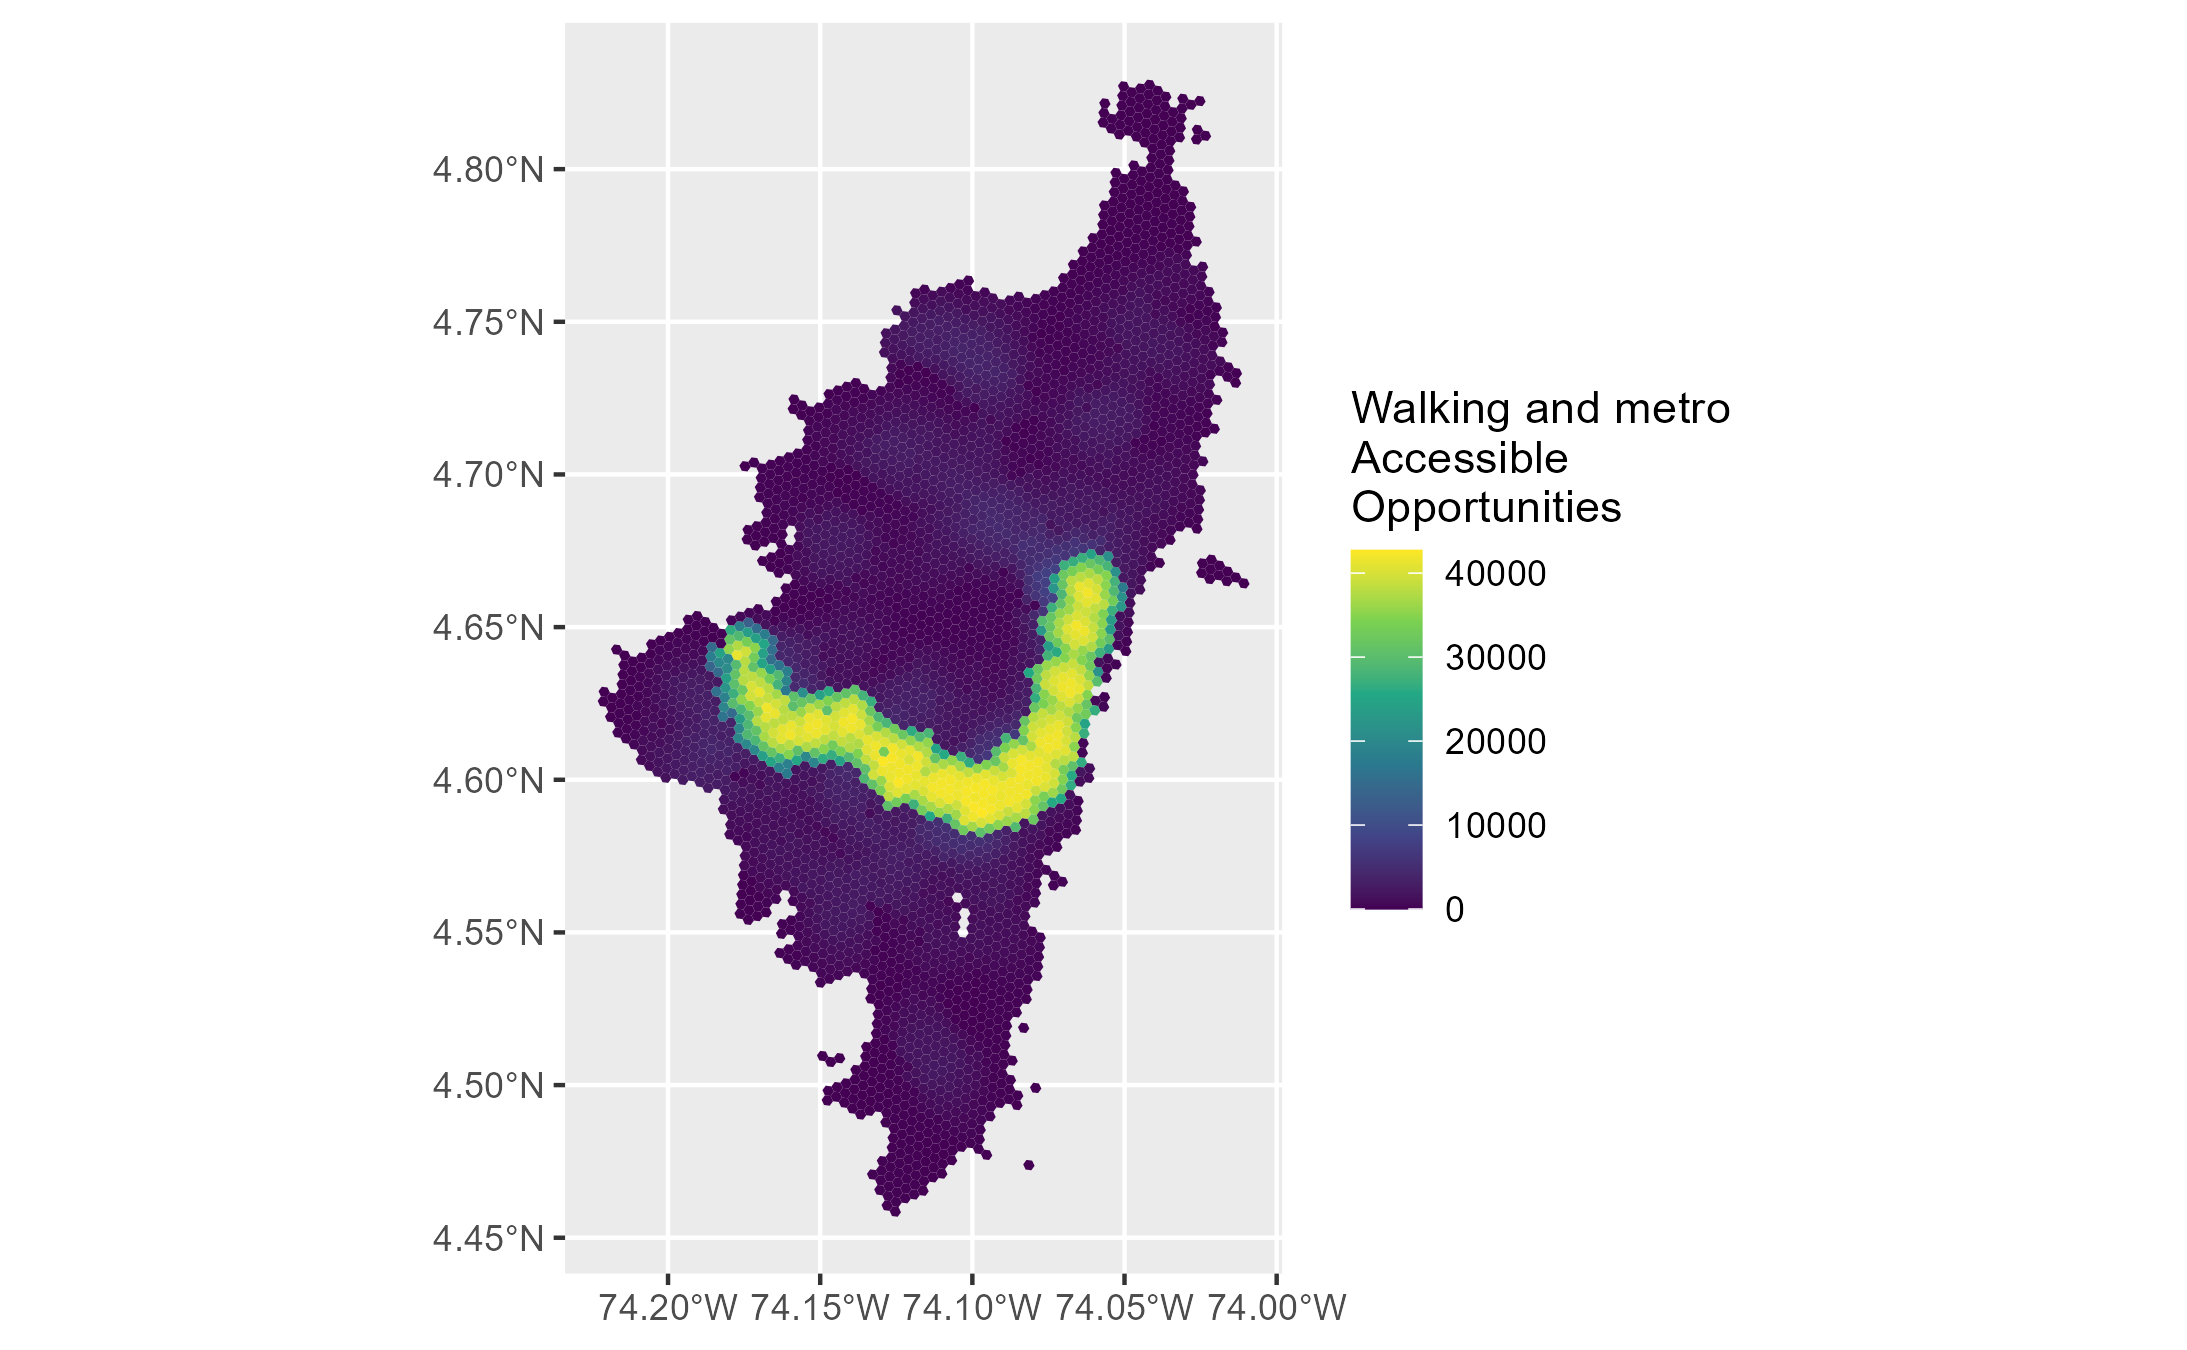
\includegraphics[width=1.3\linewidth]{Data/Results/Images/Access_Metro_base.png}
        \caption{Metro}
        \label{fig:Results_Metro_Base}
    \end{minipage}
    \begin{minipage}{0.45\textwidth}
        \centering
        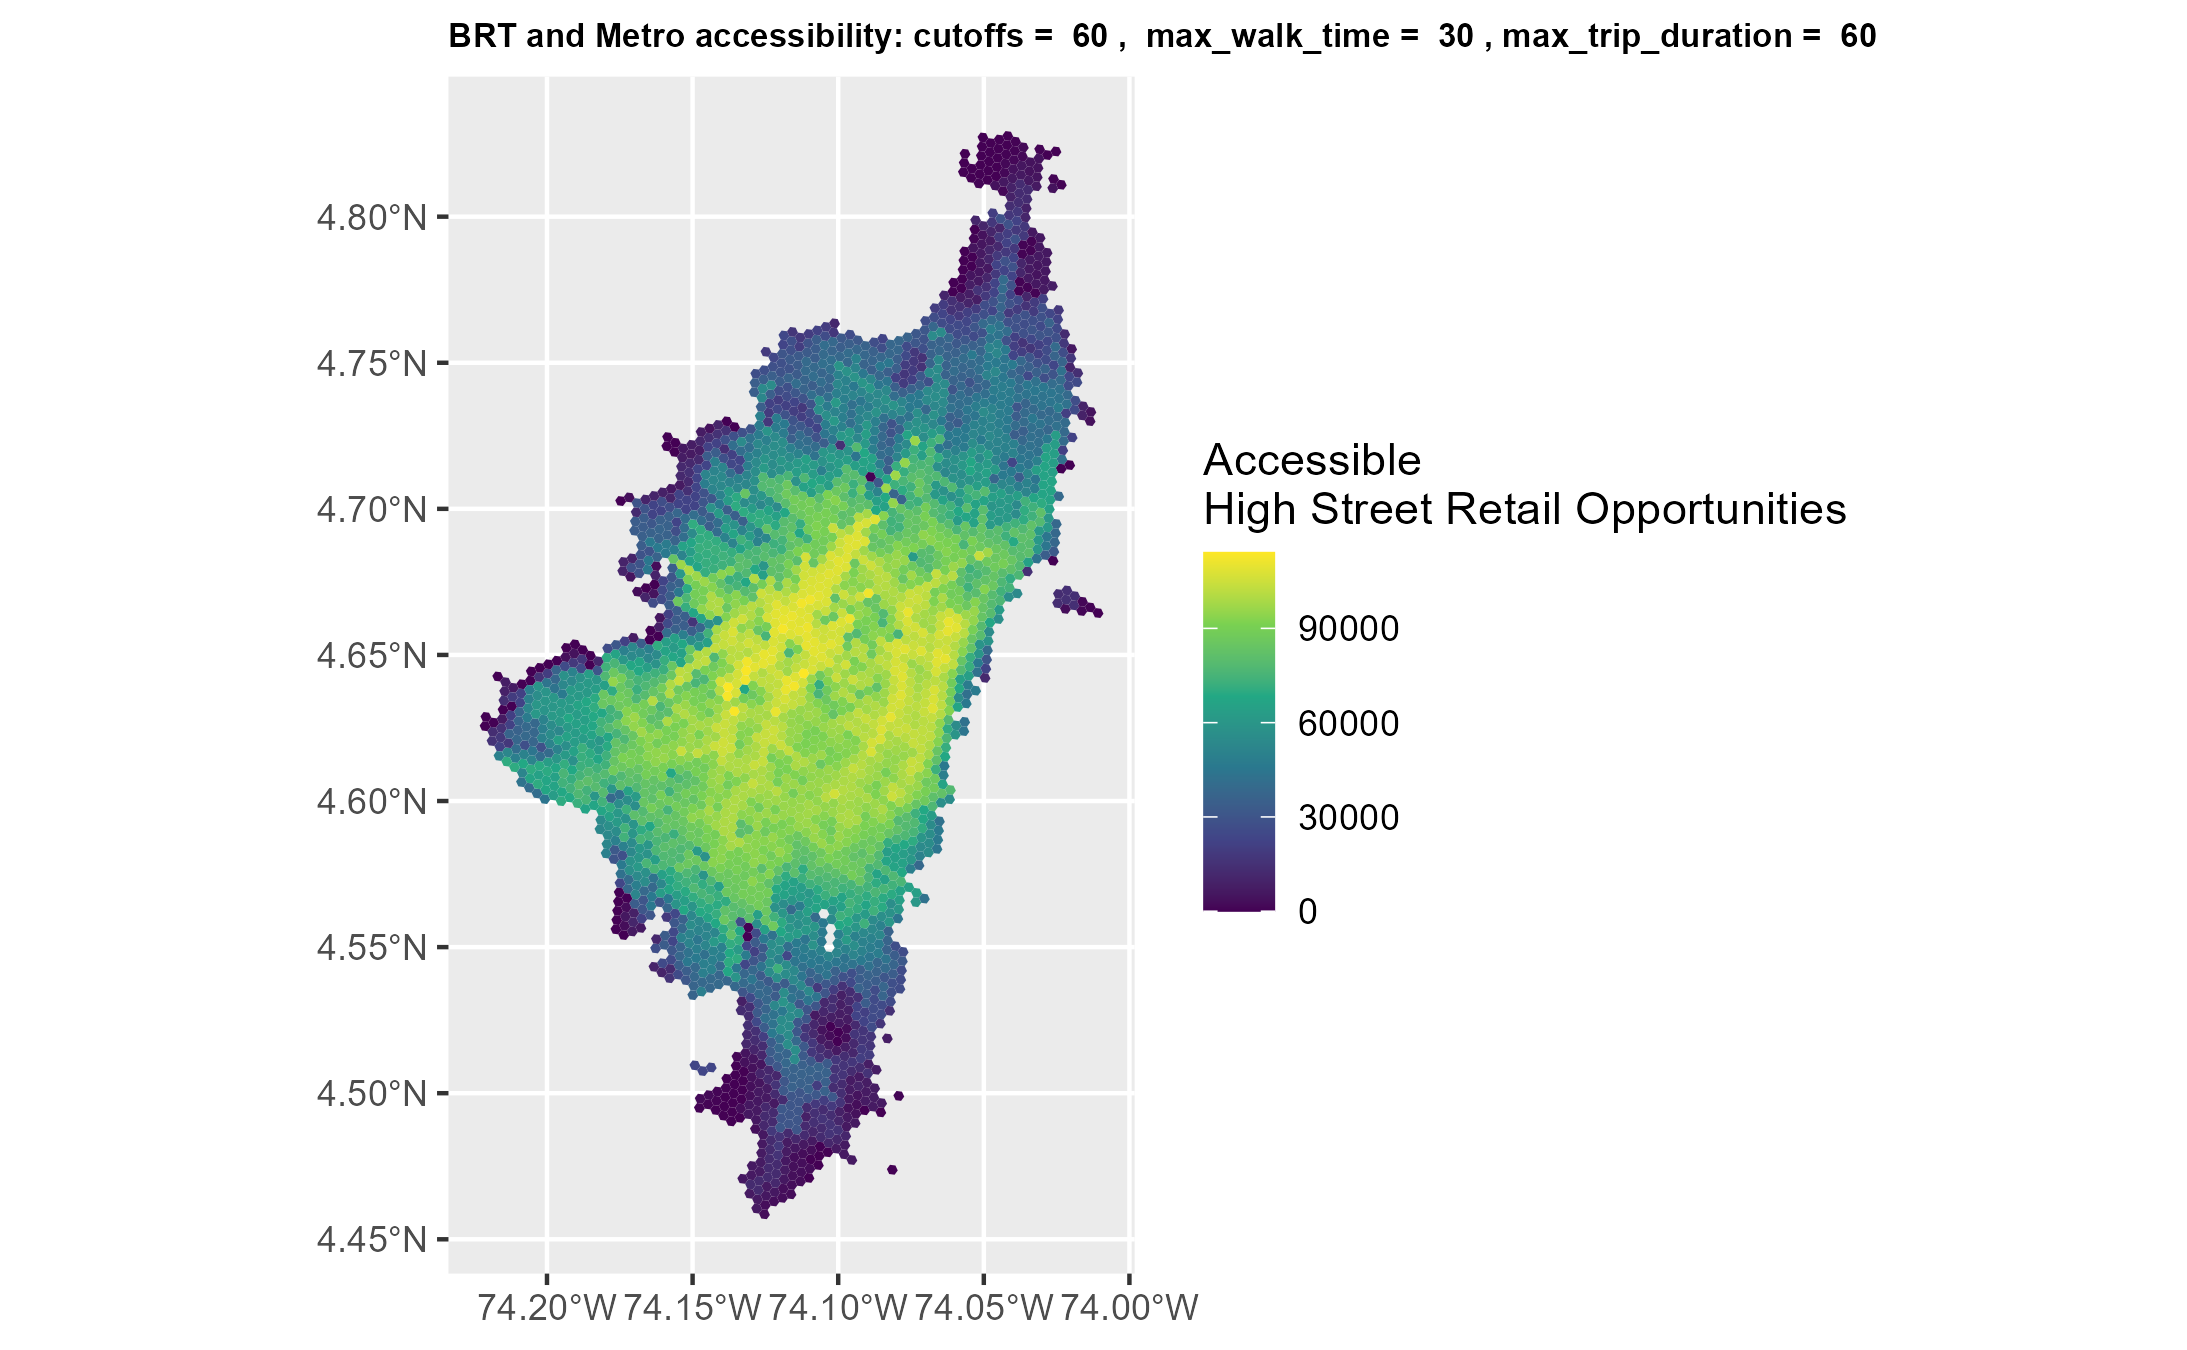
\includegraphics[width=1.3\linewidth]{Data/Results/Images/Access_BRT_Metro_base.png}
         \caption{BRT and metro}
        \label{fig:Access_BRT_Metro_Base}
    \end{minipage}    
\end{figure}

In like manner, the future scenario recreates the future accessibility situation, combining the current BRT operations with the estimated transit metro operations. \ref{fig:Access_BRT_Metro_Base} geographically represents the accessibility results for the aggregate transit conditions as if both BRT and metro were currently working. To better assess the locations that benefited the most in terms of accessibility from the metro operation, the accessibility variation between before and after scenarios was calculated. 

\begin{figure}[H]
    \centering
    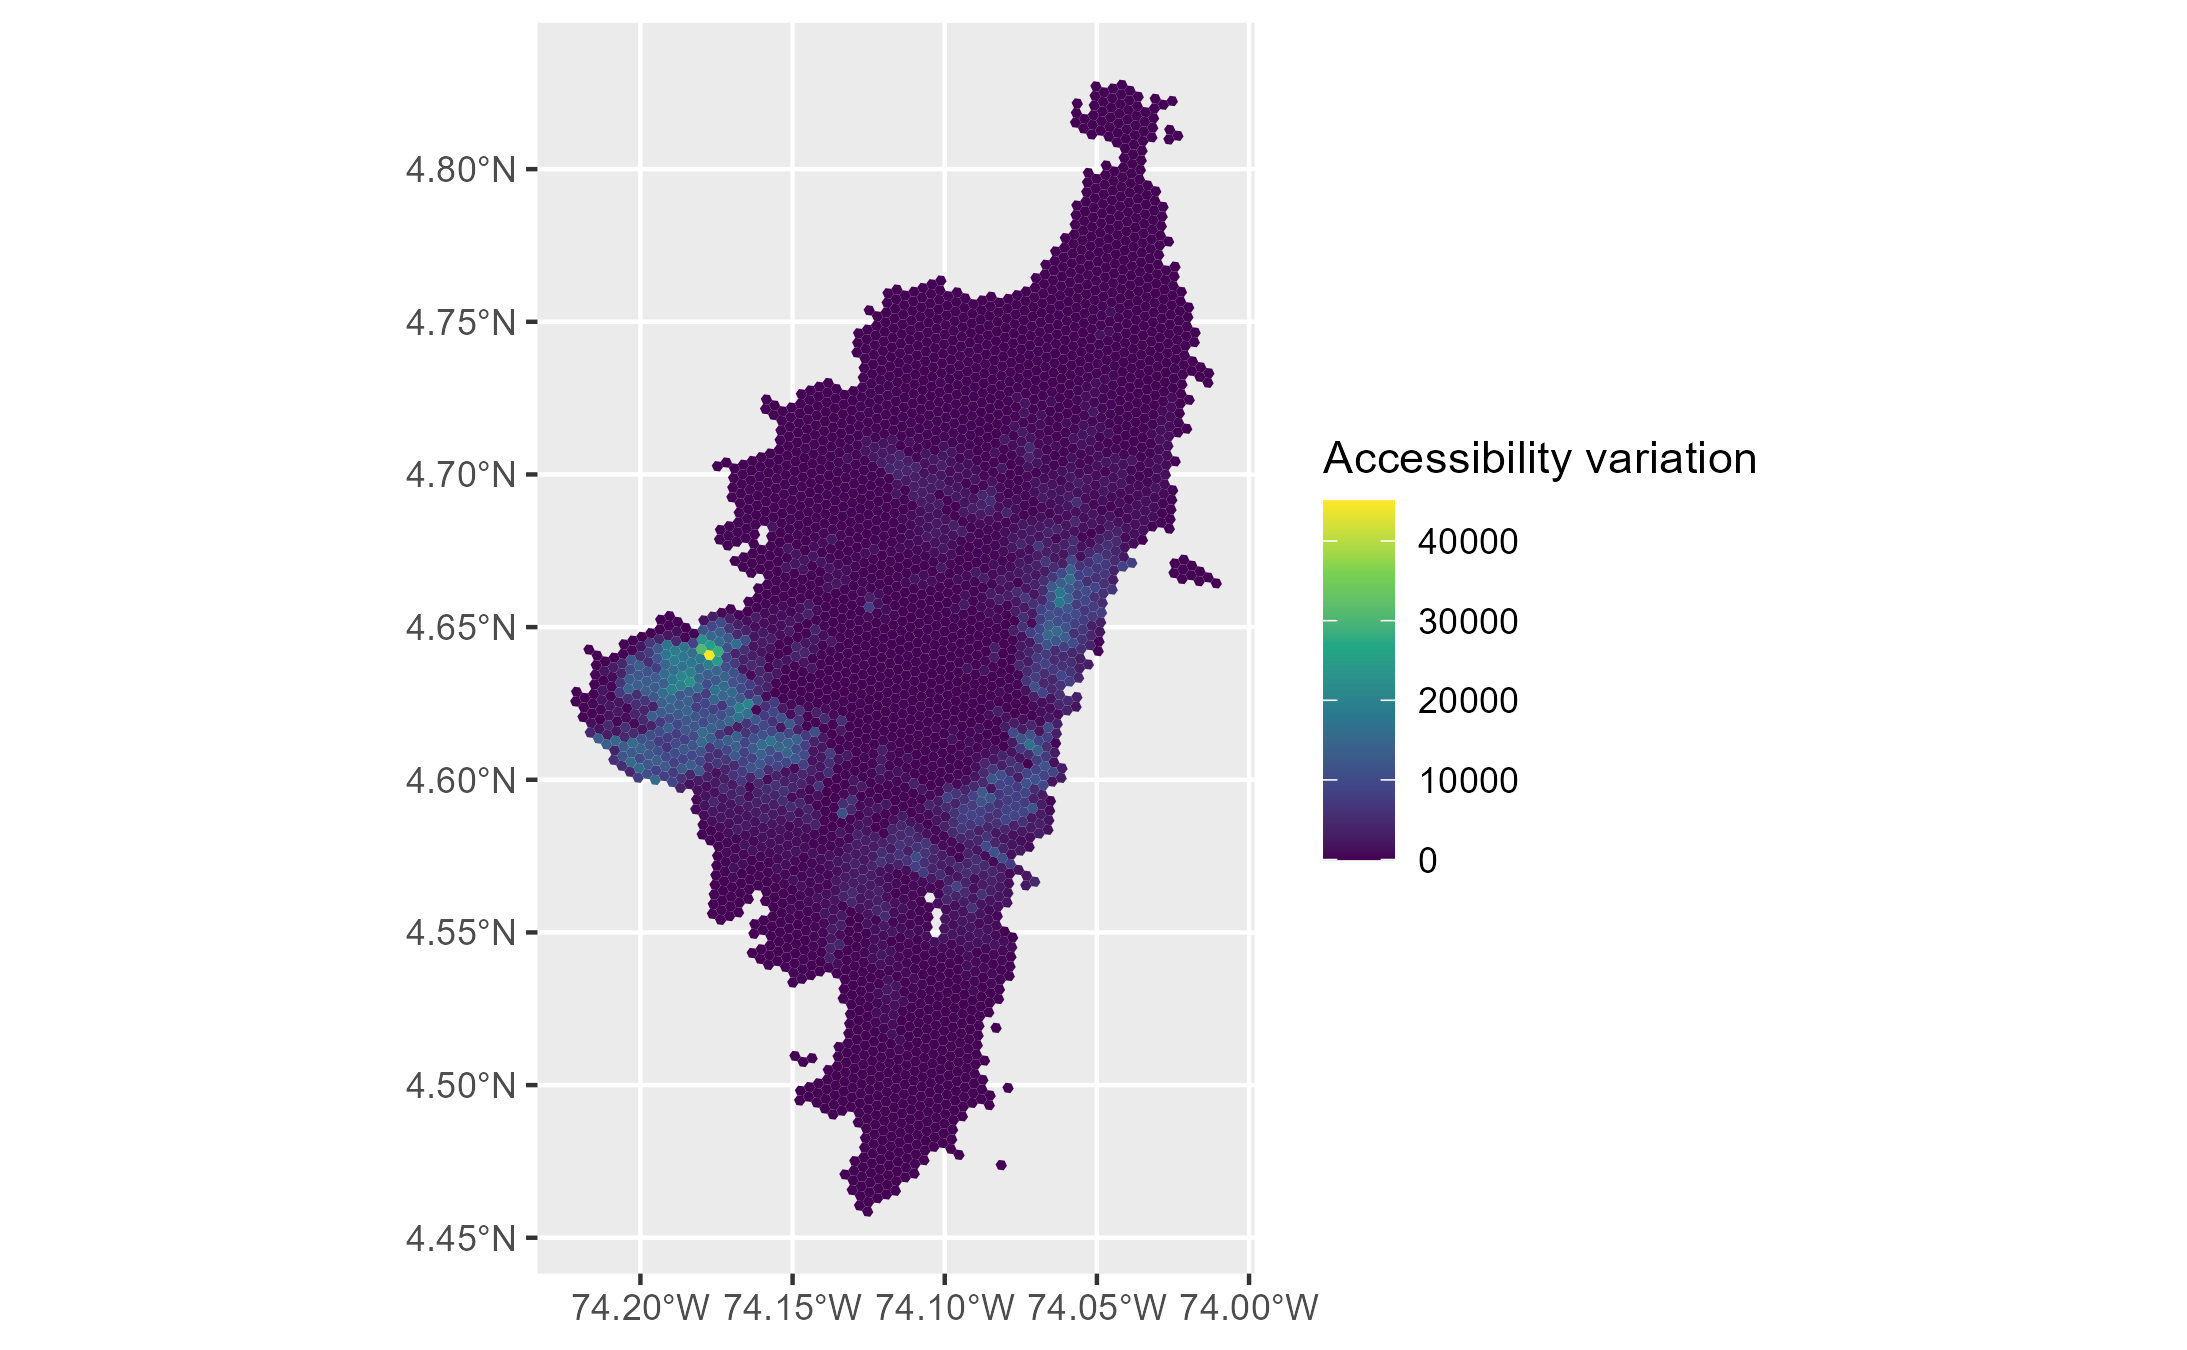
\includegraphics[width=14cm]{Data/Results/Images/Access_diff_BRT_Metro_base.png}
    \caption{Current and future scenario accessibility variation}
    \label{fig:Access_Variation}
\end{figure}

Figure \ref{fig:Access_Variation} shows the locations with the highest accessibility variation in the future scenario. These locations can be classified into three groups, each group with its particular circumstances, as described next:

\begin{itemize}
    \item Western area: The west area experienced the highest accessibility increase in the city. The accessibility increase was registered in two angles. First, the west zone had the polygon with the highest accessibility increase. The highest accessibility variation value was registered near the first station when travelling west to east on the northbound route. Second, the west Bogotá area had the largest group of adjacent hexagons, with a significant increase in Bogotá. Particularly in this area, the future metro transit operation, together with the current BRT operation, causes both situations as it allows to reach a larger opportunity number within the 30-minute walk and 60-minute total duration thresholds.
    \item Southeast area: Locations in the southeast area presented positive variations in accessibility. The increase in magnitude and the number of adjacent hexagons is less compared to the western area. The southeast area was in a relatively better accessibility situation than the western area as more opportunities were already nearby. As a result, the accessibility impact in the southeast area was less compared to the western area.
    \item Eastern area: Similarly to the southeast area, the east zone experienced increased accessibility. Locations in the eastern area had slightly higher variations than the southeast area, although the highest variations in Bogotá are still in the western area. The barely superior values in the eastern area compared to the southeast are mainly explained by more opportunities.
\end{itemize}

To more easily understand the overall accessibility impact of the metro transit operation, the distributional features of the accessibility value can be analyzed in each scenario. Figure \ref{fig:Boxplot_Access_Scenarios} shows the distribution of the accessibility results in a boxplot format for each scenario. When disaggregated, both walking and metro show possible outliers. These cases might be related to atypical privileged locations for each mode, either related to being close to the opportunities or near the metro stations, respectively. When the BRT and the metro transit operations are combined in the future scenario, the resulting distribution shows a significant increase in accessibility, particularly in the median and upper quartile. Regarding the median accessibility variation between scenarios, it expanded from 59.682 to 63.213 opportunities, which represents a 5,9\% increase. Similarly, the upper quartile value increased by 4.3\% from 86.057 to 89.743 opportunities.

\begin{figure}[H]
    \centering
    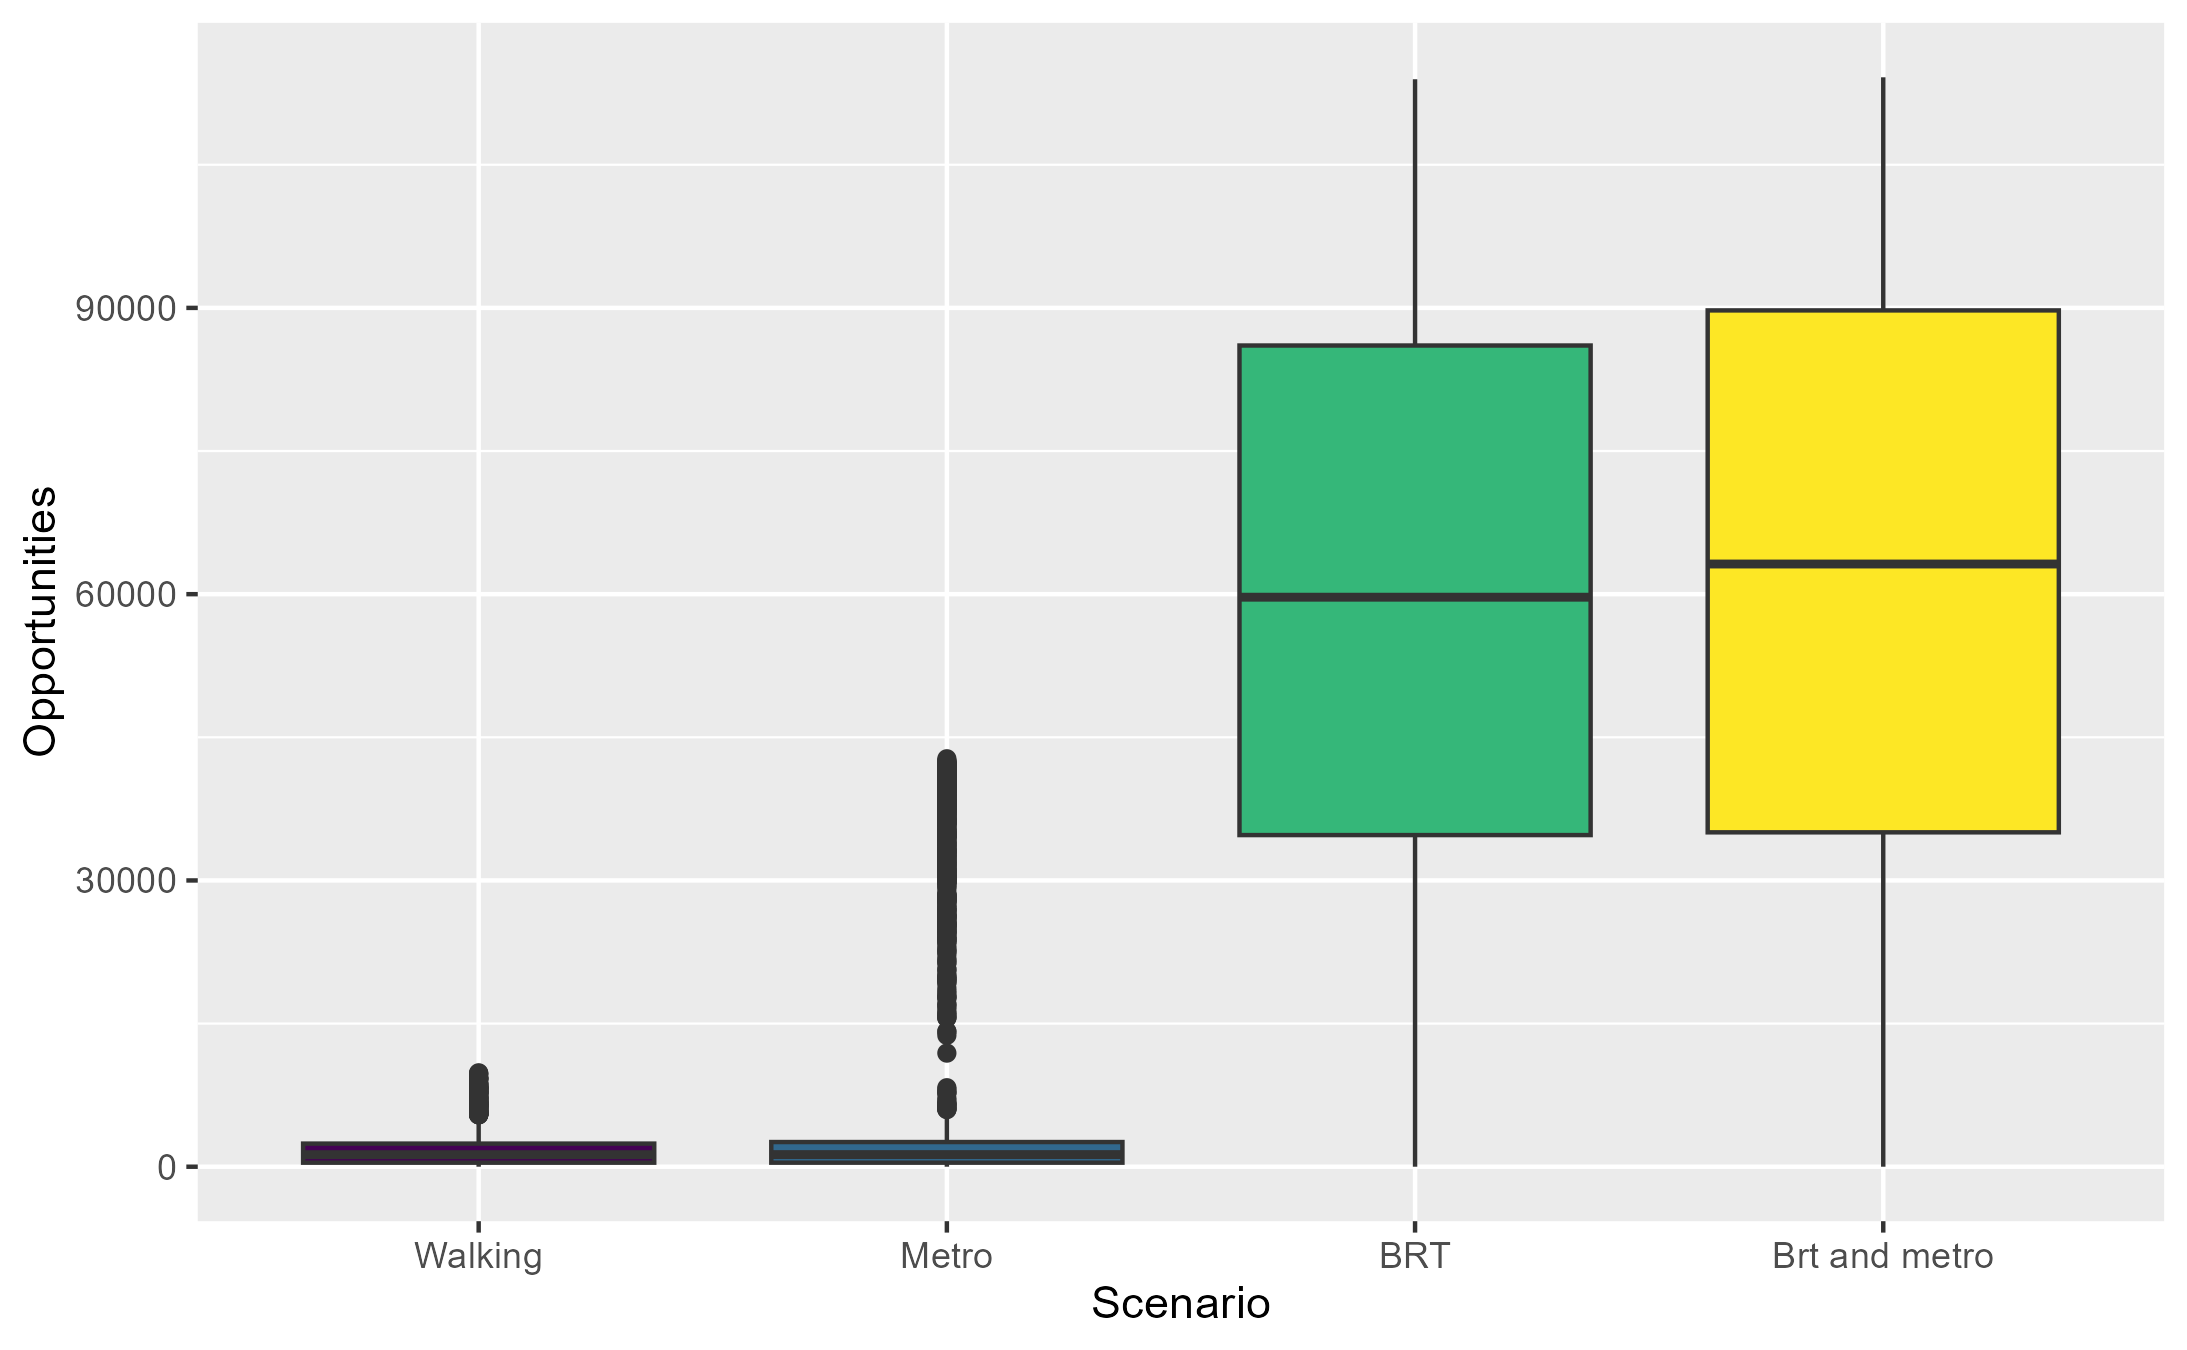
\includegraphics[width=8cm]{Data/Results/Images/Boxplot_Access_Scenarios.png}
    \caption{Accessbility results boxplot by scenario}
    \label{fig:Boxplot_Access_Scenarios}
\end{figure}

\section{Income groups}

As part of assessing the results, this study examined the modelled accessibility values by the income level reported in each location across the study area. The income disaggregation analysis enables exploring which locations benefit the most and what socioeconomic conditions have been identified \citep{pereiraIntroductionUrbanAccessibility2023a}. As the demographic data has shown previously in section \ref{Demographics}, locations with reported high income were located in the north part of the city, while locations with low-income earners were in the south, southwest and west areas of Bogotá. In this case, the first and tenth deciles would represent locations with the poorest and the wealthiest level of income. 

In the current scenario, the locations with the lowest accessibility median results were the first and second decile locations groups. On the contrary, the locations with the highest median accessibility result were the fifth, sixth and seventh income decile groups. Figure \ref{fig:Access_Income_Before_After} shows the accessibility results by income decile for the before and the future. In that particular order, the income-grouped locations with the greatest single increases were the second, fourth, first and second. Overall, the income decile with the highest increase in the accessibility median is the third decile, which represents the locations with the third lower income level reported.

\begin{figure}[ht]
    \centering
    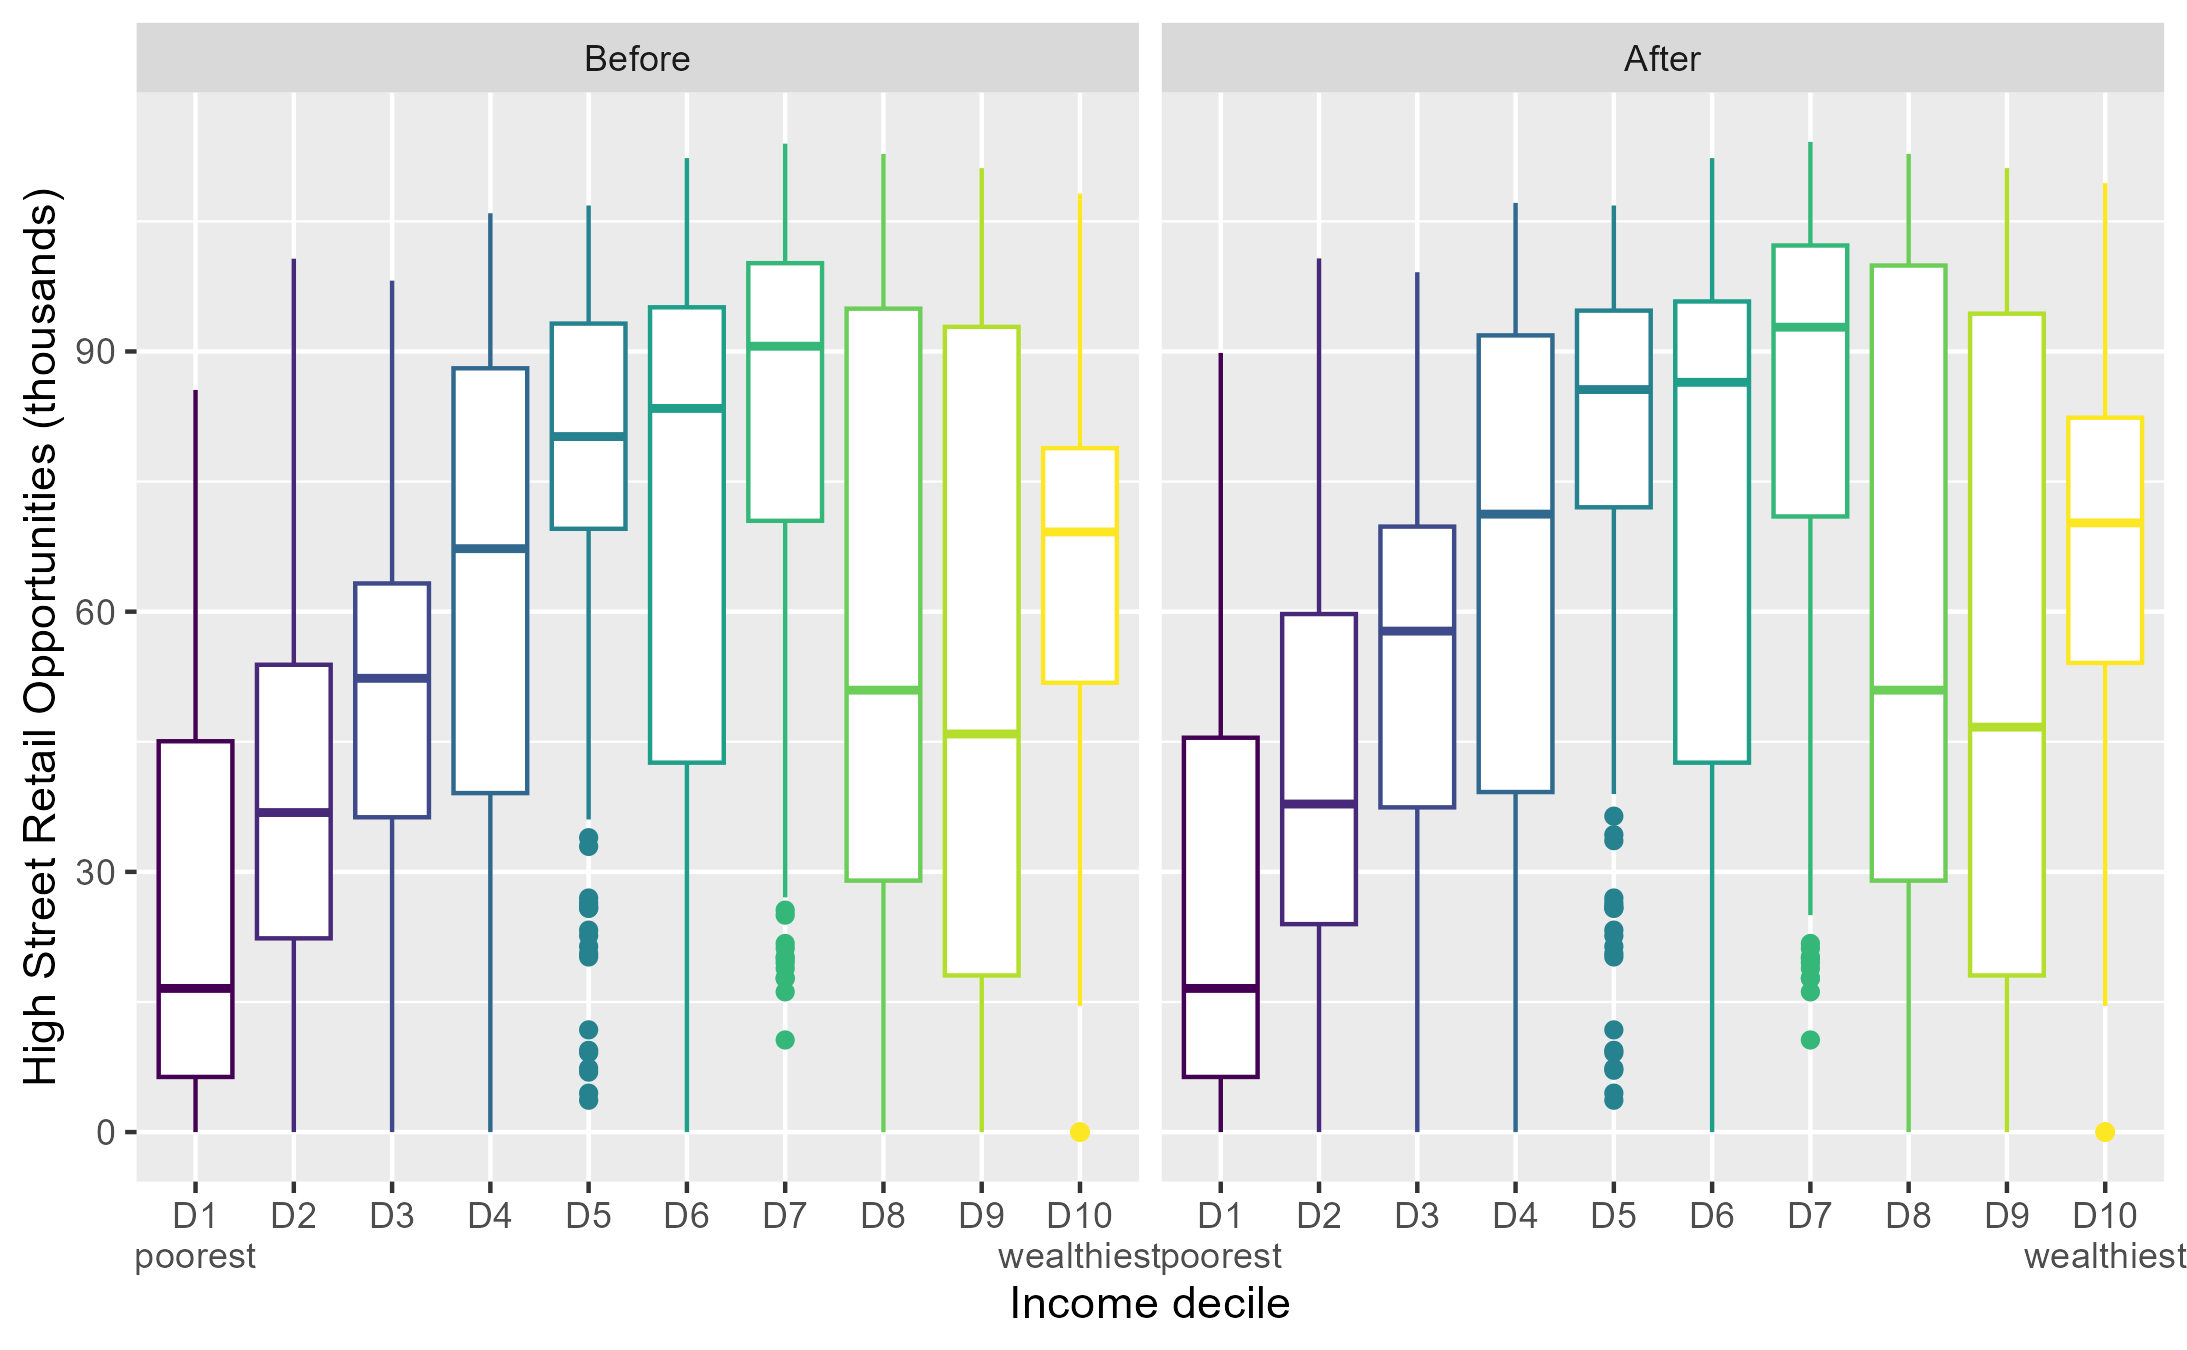
\includegraphics[width=13cm]{Data/Results/Images/Boxplot_Access_All_by_income_decile.png}
    \caption{Current and future accessibility by income decile}
    \label{fig:Access_Income_Before_After}
\end{figure}

\begin{figure}[ht]
    \centering
    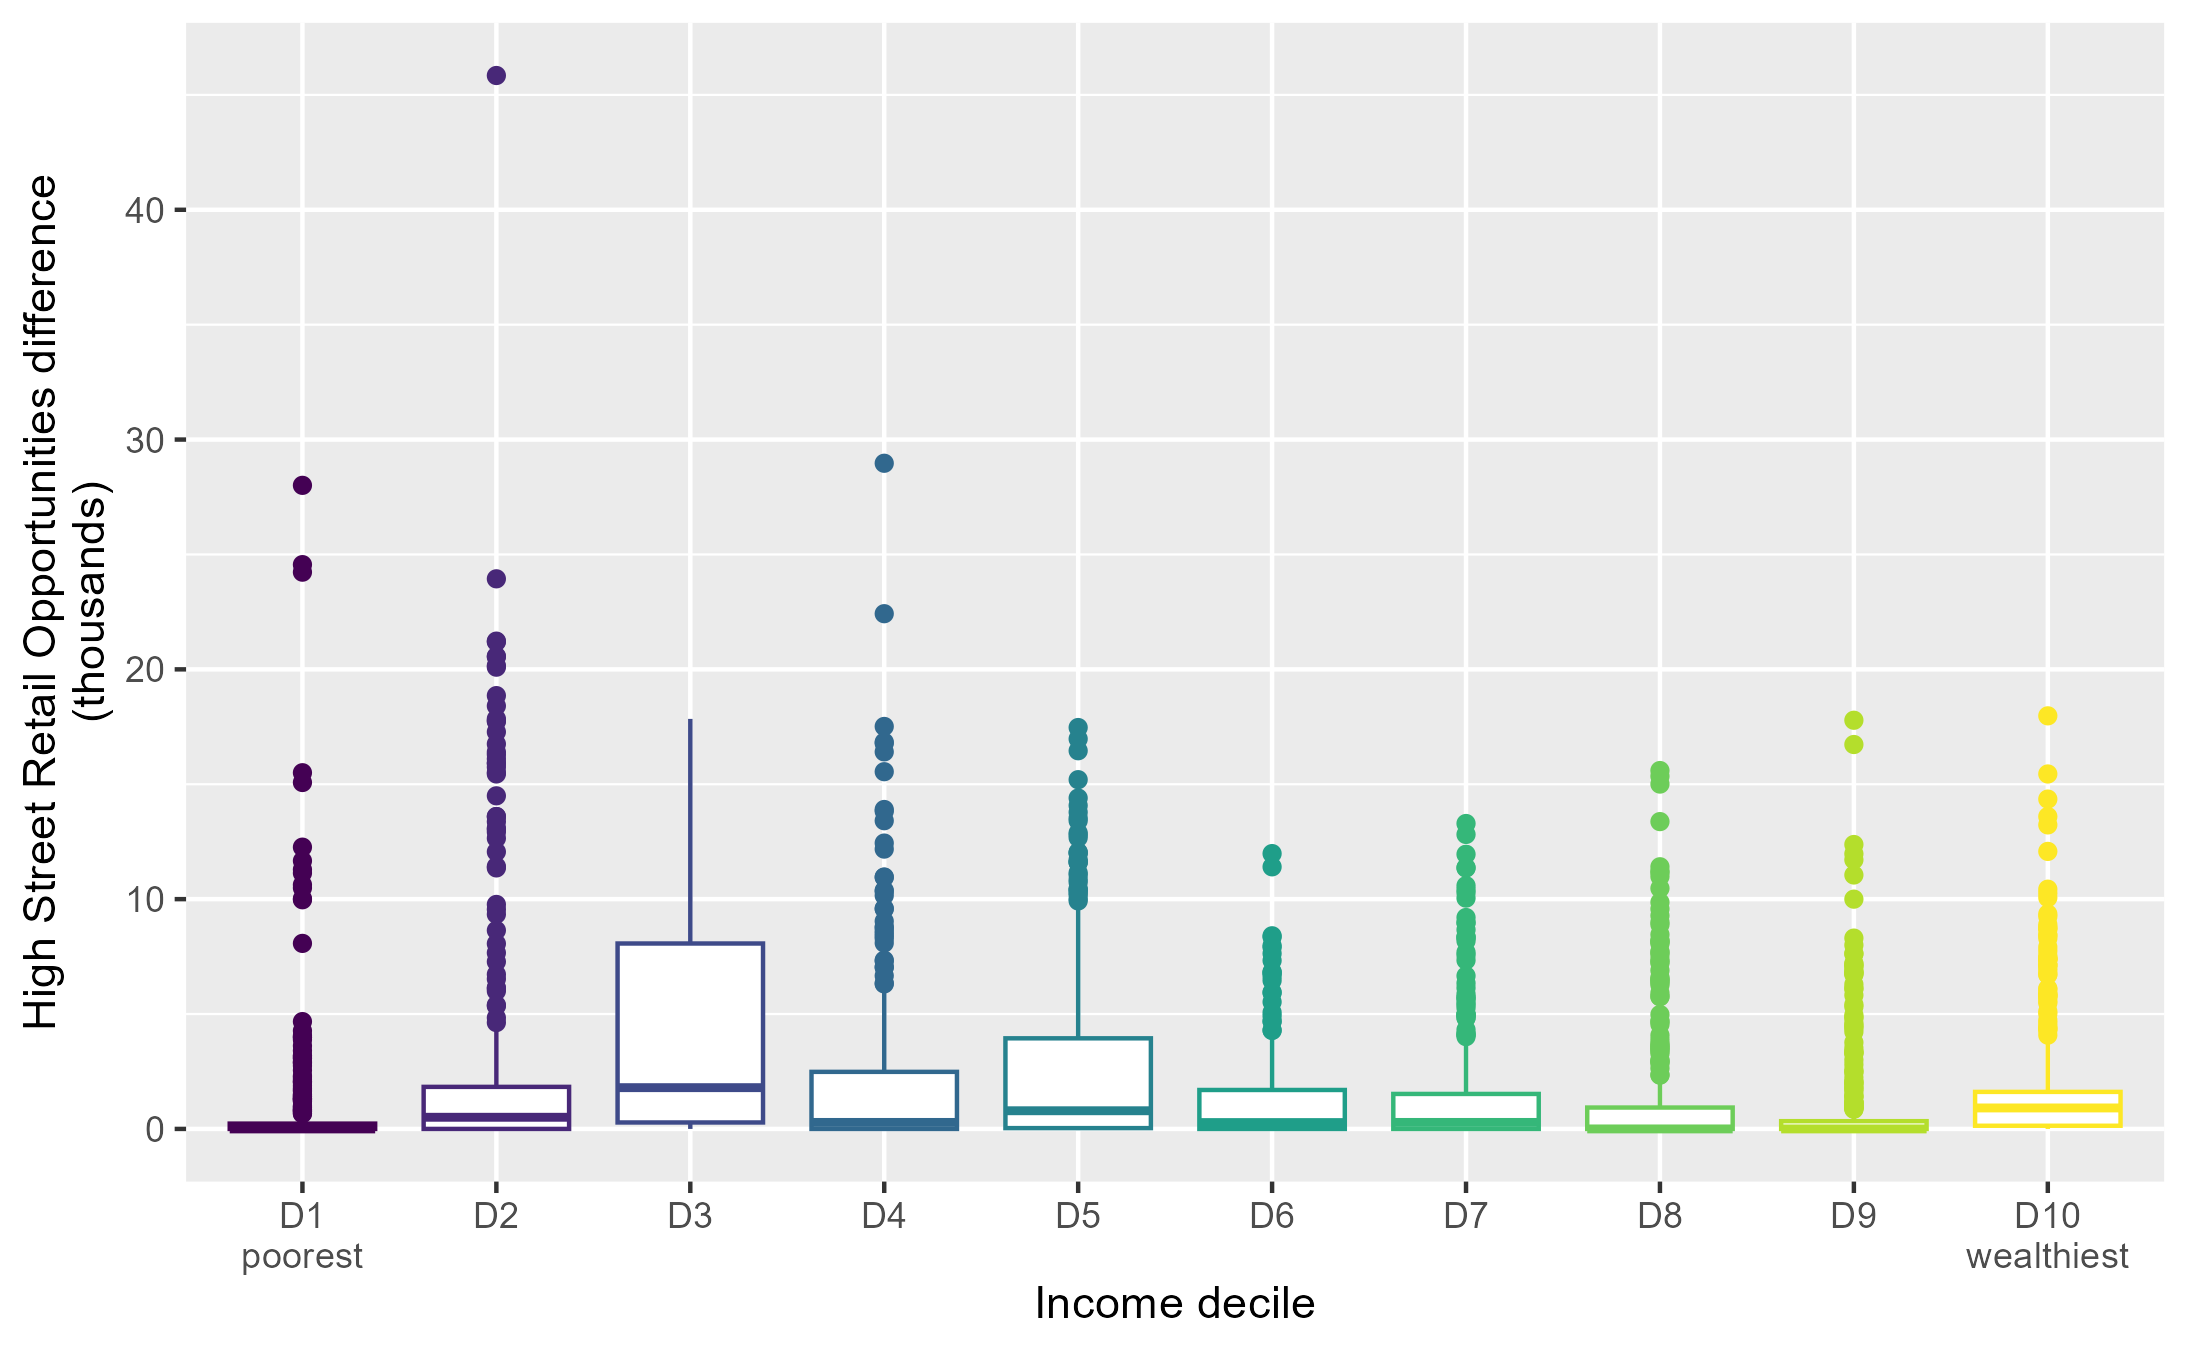
\includegraphics[width=13cm]{Data/Results/Images/Boxplot_Access_diff_by_income_decile.png}
    \caption{Accessibility variation by income decile}
    \label{fig:Access_Income_Before_After_Variation}
\end{figure}



\chapter{Discussion} \label{Chap6}

The research exercise aimed to address the following research question: 

\begin{center}
    \textit{How would Bogot\'{a}\textquotesingle s future metro line contribute to improving access to opportunities?} 
    %How would the public transportation accessibility spatially vary with the construction of Bogot\'{a}\textquotesingle s future metro system?}
\end{center}

The research question was addressed by recreating the transit circumstances, modelling the number of reachable opportunities and comparing the accessibility results between the current and the future scenario. This study spatially assessed how the future metro infrastructure and transit operation and the already functioning BRT system would increase the number of reachable opportunities. A novel feature of the study was the creation of the transit specification for the metro service in GTFS format, considering that the first line is supposed to start operations in 2028. Furthermore, this study examined the future accessibility impact by disaggregating the results by the income level reported in each location in Bogotá.

The study generated results that show the overall increase in accessibility, where this is more intensely happening, and what population groups benefit the most in terms of accessibility with the construction of the first Bogotá metro line.


Regarding the reproducibility of this study, the code used to conduct the data analysis, preprocessing, modelling, and visualization is available in this \href{https://github.com/rpoandres/MSc_USS_Dissertation}{repository}, together with the maps and figures included in this document.

\section{Implications}

\subsection{Transit assessment}

This study expanded the use of accessibility measures to spatially and socioeconomically assess the tangible benefits related to a transport infrastructure project \citep{bocarejos.TransportAccessibilitySocial2012,bocarejoAccessibilityAnalysisIntegrated2014,guzmanAssessingEquityTransport2017}. As accessibility modelling better integrates, both transit offers and the reachable locations of interest (opportunities), its use should be adopted by transport planning practitioners instead of considering standalone mobility-driven measures to support transport decision-making processes \citep{ferreiraAccessibilityGoldMobility2012}. It is important to realize that with the mere use of travel time analysis when assessing the impact of the future metro, the measure would have fallen short in reckoning the value of reaching new opportunities with the same commuting constraints.

The method developed in this study models and analyses accessibility to any location of interest. This versatile feature of the methodology allows for conducting a multi-layer accessibility assessment. In that sense, accessibility assessment could account for a multi-opportunity type assessment depending on the specific circumstances and research purposes. An opportunity can entitle a location related to education, health, jobs and leisure. In other words, for any location of interest in the study area, an accessibility measure could be computed and reviewed individually or collectively when strategically assessing the suitability, sustainability and social inclusion of transportation-related projects \citep{pereiraIntroductionUrbanAccessibility2023a}. By having this multipurpose accessibility measure platform, the transport planning decisions can more easily be framed as part of initiatives that contribute to SDG \# 11 'Make cities and human settlements inclusive, safe, resilient and sustainable' \citep{unitednations17GOALSSustainable2015}. Furthermore, with the demographic disaggregation of results, in this case, done income decile, it is possible for local authorities and transport planning decision-makers to prioritize and allocate resources strategically to targeted population groups who might be experiencing a  more vulnerable and disadvantaged situation.


\subsection{Future alternative scenario modelling}

The research contributed to enabling the tools for facilitating alternative scenario modelling in addition to the already modelled future metro scenario. This study examined the future metro scenario and the current BRT transit operation as a standalone possibility following the transit operations' estimated performance and the physical location of the metro infrastructure. However, a wide range of modelling accessibility opportunities can be easily covered by expanding the spectrum of alternative scenarios. By including new alternative scenarios and expanding the input data, this study can be scaled to model accessibility under new transit circumstances systematically.

The new alternative scenarios could rapidly provide insight into the impact of accessibility by modifying commuting duration thresholds, route paths, frequencies, timetables, and number of stations, among other transit specifications. As several inputs in the modelling process are structured based on general operational assumptions of the non-existent metro system, the inputs can be restructured and multiple alternative scenarios by modifying this assumption. An example of this is the relation between the travel speed of the metro and the timetables of the trips. The arrival and departure time schedules are constructed based on the stations' geographical location and the metro's expected travel speed. To follow the example, the tools employed in this study could deployed to replicate new possible versions of the system by changing the locations of the stations and/or the travel speed of the metro. This logic of simulation and experimentation workflow falls accurately into the outlook portrayed by \cite{wilsonFutureUrbanModelling2018, battyUrbanModeling2009a,longleyGeographicInformationScience2015} where urban modelling supported by geographic information system provided a digital to test and estimate variables of interest in future scenarios. 


\section{Future research}

\subsection{New measure possibilities}


Regarding the further expansion of accessibility-driven measures, stating accessibility measures as the basis, platform and backbone of transport-related planning brings a wide range of new measures derived from accessibility. An example is ratios that could be calculated when designing a future transit operation or assessing an existing one. 

By measuring the relationship between accessibility measures and other relevant measures related to transport through a ratio, they could contribute to a more informed decision as the ratio variables reflect both accessibility and strategic features of the project. The combination of accessibility-based measures and other components of the projects can more easily articulate the project stakeholders around the same social-equality-oriented accessibility strategy. As an illustration, a ratio between the increase in accessibility and the cost of increasing the carrying capacity of the metro, measured in passengers per hour per direction, can establish a cost-benefit relation between accessibility gains and the construction cost per kilometre. The same ratio exercise can be done with operational, financial and transit variables. Ultimately, an accessibility-based ratio will contribute to a more accessibility-aware culture and promote their use in any transport-related decision.

\subsection{Additional transport modes}

This study employed a multi-transport methodology that could be expanded to additional transport modes. As urban mobility includes more diversity in commuting modes, such as active travel modes \citep{malteseActiveTravelSustainable2021}, so can the accessibility modelling process. As \citep{alcaldiadebogotad.c.EncuestaMovilidad20192019} showed modes like scooters and bicycles are also an alternative when commuting in Bogotá. Using non-carbon motorized vehicles for daily commutes reduces the transport sector's impact, considering that this sector faces structural challenges to achieve decarbonization status. Measuring the cycling accessibility results and decreasing carbon-based mobility would integrate an active mode of transport with a climate change-related initiative. Likewise, the link between accessibility and an active travel model, used exclusively or combined with other modes, can quantify the environmental and accessibility cost-benefit relationship. 


\subsection{Opportunities data refinement}

The opportunity preprocessing procedure of the land use aggregation accounts for the number of terrains located in a land use category in a given location (hexagon grid) in Bogotá. Among the features or attributes related to each terrain, some variables can contribute to assessing the magnitude or importance of each opportunity more accurately. The area or the number of levels in height construction, combined with the land use category, can help dimension the number of opportunities that a particular terrain can hold. An example is when big commercial developments are developed in high-level construction or holding multiple commercial units within one standalone terrain. By using the leasable commercial area and the number of levels of construction, the land use area could more precisely reflect the real number that one single terrain can hold. Additionally, grouping between the different land use categories can be made. For example, residential and non-residential land use can be linked to the distinct density of possible job opportunities. Furthermore, within the non-residential group, each land use could contribute differently to accessibility depending on the type of opportunities included in the research exercises. In a word, land use data preprocessing could reflect additional features to more precisely assess the number of opportunities.

\section{Limitations}

\subsection{Demographic data resolution}

The scale of spatial aggregation from the demographics data limits the accuracy of the assessment of the results. As shown in \ref{fig:Study_Area_ZPU}, Bogotá is administratively divided into 112 ZPU\footnote{For consistency purposes, the map shows 96 ZPU as aggregated in the Muliprpuse Survey, although there are official 112 \citep{secretariadistritaldegobiernoCaracterizacionUsuarios20212021}} and that same spatial aggregation is used to georeference the demographic data to disaggregate the accessibility results. The size of the ZPU polygons compared to the size of the resolution 9 hexagon grid cells is superior. As the demographic data is spatially referenced using the ZPU polygons, the spatial interrelation between the accessibility results and the demographic data (e.g. income) weakens when the size of the initial layer of the data exceeds the size of the spatial analysis unit used for the spatial aggregation process. The spatial aggregation procedure was performed despite this limitation, and the results showed consistency within the values used in the results assessment process.

\subsection{Transit conditions and assumptions}

The transit operations reported by the current BRT operation could be rescaled in some cases to better reflect a more realistic transit operation together with the current level of demand for the BRT transit service. In specific features of the GTFS data used by this study to replicate the BRT transit operation, an adjustment procedure can be done to more accurately and realistically simulate the daily transit operation in Bogotá. One case identified was the timetable structure in the stop times table in the BRT GTFS data. According to the data contained in the GTFS data, the arrival and departure time of the BRT service is the same. That means there is no time reserved for the boarding of passengers. The disembarking of passengers is an activity that consumes time and should be considered in operation, especially as the BRT has consistently reported high congestion levels in high-density corridors \citep{guzmanDensityorientedPublicTransport2021}. Although this unrealistic situation was identified in the GTFS data, the same situation was replicated in the metro transit operation to prevent the metro from artificially losing and competing against the BRT operations. Given these points, to assess the mode choice more realistically, both BRT and metro modes should account for interrelated congestion conditions for future research.

\chapter{Conclusion} \label{Chap7}


Bogot\'{a} has doubled in population during the last 30 years \citep{guzmanCityProfileBogota2017}. The current size and future population growth of Bogotá intensify the urgency to generate more liveable and sustainable spaces. For this reason, strengthening more sustainability-oriented transport and planning decision-making processes is urgently required. The method employed systematically combined the transport infrastructure and Bogotá's future and current transit operations with the spatial distribution of opportunities to model how accessible those opportunities were. The methodology considered mobility conditions as the commuting time between origins and locations in Bogotá and measured what those commuting circumstances meant regarding access to opportunities. 


The results were first examined spatially across Bogotá for each scenario to address the research question. Later, overall results were comparatively plotted to understand their distribution and structural differences between scenarios. The accessibility spatial results showed that the western area of Bogotá would experience the highest increase in accessibility when the first metro line transit operation starts, functioning together with the current BRT transit operation. The city's western area presented the highest positive variation in accessibility combined with the largest group of adjacent locations with a significantly high accessibility increase. Although the western area had a relatively lower number of opportunities nearby, the metro transit operation enabled opportunities to be reached within a 30-minute walking and a total 60-minute commuting limit. 

All things considered, cities and transport-related agencies can potentially use the model and the results generated to assess the performance of future or currently functioning transport with a measure that holistically integrates the real tangible access benefit to locations of interest (opportunities) when using a transportation system and can contribute to achieving more social-inclusive, liveable and ultimately, sustainable cities.

% Refecenre policy makers

\renewcommand{\bibname}{References}
\bibliographystyle{agsm}
%\bibliography{Bibliography.bib}
\bibliography{references.bib}
%%%%%%%%%%%%%%%%%%%%%%%%%%%%%%%%%%%%%%%%%%%%%%%%%%%%%%%%%%%%%%%%%%%%%%%%%%%%%%%%
% APPENDIX
\begin{appendices}
\chapter{Source code and data} \label{Source_Code}
Source code and data for all of the methods implemented in Chapter \ref{Chap4} for the project can be found in the remote repository: \href{https://github.com/rpoandres/MSc_USS_Dissertation}{GitHub}

% \chapter{Ethics review} \label{Ethics_Review}

\chapter{Supervision records}

Dr. Fulvio Lopane supervised this dissertation, and the next table lists the meetings undertaken during the supervision period:

\begin{table}[h]
\centering
\begin{tabular}{|c|c|p{6cm}|}
\hline
\textbf{Number} & \textbf{Date} & \textbf{Main topics reviewed}                                                                                      \\ \hline
1 &
  30/03/2023 &
  Based on the availability and spatial data resolution, methodological alternatives were explored. Additionally, an initial ethics screening was done to assess risk level. \\ \hline
2 &
  16/05/2023 & The initial list of activities and the main structure of the document were reviewed. Related literature and potential additional input data were mentioned.\\ \hline
3               & 22/06/2023    & Progress update on the R5R library review. Initial structure of literature review section was also reviewed.       \\ \hline
4               & 13/07/2023    & Update on the preprocessing code, the BRT route geometry review and the initial set of accessibility results.         \\ \hline
5               & 07/08/2023    & Updates on including the metro transport mode in the accessibility computation. List of main activities to execute. \\ \hline
6 &
  \multicolumn{1}{l|}{22/08/2023} &
  Checklist before submission review, result visual display review and exploration on what messages to include in the discussion section. \\ \hline
\end{tabular}
\end{table}




% \chapter{Project Introduction Video}\label{sec:projectIntroduction}
% A short video presentation, introducing background, aims and organisation of the project, as of 30$^{th}$ June 2022: \newline
% \url{link}



\end{appendices}
%%%%%%%%%%%%%%%%%%%%%%%%%%%%%%%%%%%%%%%%%%%%%%%%%%%%%%%%%%%%%%%%%%%%%%%%%%%%%%%%
% GLOSSARY
\clearpage
\printglossaries

% INDEX?

\end{document}